\documentclass[review]{siamart190516}

% Journal name: SICOMP
%\usepackage[margin=0.75in]{geometry}
\usepackage{amsmath, amssymb}
\usepackage{mathtools}
\usepackage{url}
\usepackage{enumitem}
\usepackage{setspace}
\usepackage{scalefnt}
\usepackage[utf8]{inputenc}
\usepackage[english]{babel}
\usepackage{algorithm}
%\usepackage{algorithm2e}
%\usepackage{algorithmicx}
\usepackage[noend]{algpseudocode}
\usepackage{bbm}
\usepackage{graphicx}


\newcommand\sbullet[1][.5]{\mathbin{\vcenter{\hbox{\scalebox{#1}{$\bullet$}}}}}
\usepackage{blkarray, bigstrut}
\usepackage{tikz}
\usetikzlibrary{arrows.meta, calc, quotes, tikzmark,shapes}

\usepackage{caption} 
\captionsetup[table]{skip=4pt, position=above}

\usepackage{array}
\newcolumntype{P}[1]{>{\centering\arraybackslash}p{#1}}

\newcommand\topstrut[1][1.1ex]{\setlength\bigstrutjot{#1}{\bigstrut[t]}}
\newcommand\botstrut[1][0.95ex]{\setlength\bigstrutjot{#1}{\bigstrut[b]}}

\makeatletter
\newcommand{\customlabel}[2]{%
   \protected@write \@auxout {}{\string \newlabel {#1}{{#2}{\thepage}{#2}{#1}{}} }%
   \hypertarget{#1}{#2}
}
\makeatother

\newcommand\undermat[2]{%
  	\makebox[0pt][l]{$\smash{\underbrace{\phantom{%
    \begin{matrix}#2\end{matrix}}}_{\text{$#1$}}}$}#2}

\usepackage{hyperref} % load hyperref last

%\newtheorem{theorem}{Theorem}
%\newtheorem{definition}{Definition}
%\newtheorem{proposition}{Proposition}
%\newtheorem{lemma}{Lemma}
%\newtheorem{corollary}{Corollary}
% \newcommand{\CommentX}[1]{\unskip~\%~#1~\%}

\newsiamremark{remark}{Remark}

\DeclareMathOperator*{\argmax}{arg\,max}
\DeclareMathOperator*{\argmin}{arg\,min}
\DeclarePairedDelimiter\ceil{\lceil}{\rceil}
\DeclarePairedDelimiter\floor{\lfloor}{\rfloor}

\usepackage{outlines}
\usepackage{enumitem}
\setenumerate[1]{label=\arabic*}
\setenumerate[2]{label*=.\arabic*}
\setenumerate[3]{label*=.\arabic*}
\setenumerate[4]{label*=.\arabic*}

% Sets running headers as well as PDF title and authors
\headers{Fast Persistence Computations}{M. Piekenbrock and J. Perea}

% Title. If the supplement option is on, then "Supplementary Material"
% is automatically inserted before the title.
\title{Move Schedules: Fast persistence computations in coarse dynamic settings\thanks{\textbf{Funding:} This work was partially supported by the National Science Foundation through grants CCF-2006661 and CAREER award DMS-1943758.}
}

% Authors: full names plus addresses.
\author{
	Matthew Piekenbrock\thanks{Khoury College of Computer Sciences, Northeastern University.}
	\and Jose A. Perea\thanks{
	Department of Mathematics and Khoury College of Computer Sciences, Northeastern University.}
}

%\title{\vspace{-2.0em} Move Schedules: \\ Fast persistence computations in sparse dynamic settings\thanks{This work was partially supported by the National Science Foundation through grants CCF-2006661 and CAREER award DMS-1943758.}\vspace{-0.5em}}
%\author{Matt Piekenbrock\thanks{Department of Computational Mathematics, Science \& Engineering, Michigan State University}\;\; and Jose A. Perea$^\dagger$\thanks{Department of Mathematics, Michigan State University}}
%\date{}

% Optional PDF information
\ifpdf
\hypersetup{
  pdftitle={Move Schedules},
  pdfauthor={Matthew Piekenbrock and Jose A. Perea}
}
\fi

% ------  Begin document ------- 
% https://github.com/peekxc/dart
\begin{document} 
\maketitle

% REQUIRED - "Abstracts must be able to stand alone and so cannot contain citations to the paper's references, equations, etc. .... not exceeding 250 words"
\begin{abstract}
	The standard procedure for computing the persistent homology of a filtered simplicial complex is the matrix reduction algorithm. Its output is a particular decomposition of the total boundary matrix, from which the persistence diagrams and generating cycles can be derived. 
	Persistence diagrams are known to vary continuously with respect to their input, which motivates the algorithmic study of persistence computations for time-varying filtered complexes. Computationally, simulating persistence dynamically can be reduced to maintaining a valid decomposition under adjacent transpositions in the filtration order. 
	In practice, the quadratic scaling in the number of  such transpositions often makes this maintenance procedure slower than simply computing the decomposition from scratch,  limiting the application of dynamic persistence to relatively small data sets. In this work, we propose a coarser strategy for maintaining the decomposition over a 1-parameter family of filtrations. Our first result is an analysis of a simple linear-time strategy which reduces the number of column operations needed to simulate persistence across a fixed homotopy by at most a factor of 2. We show a modification of this technique which maintains only a sublinear number of valid states, as opposed to a quadratic number of states, and we provide tight lower bounds for this technique.
	Finally, we present results showing that the decrease in operations to compute diagrams across a family of filtrations is proportional to the difference between the expected quadratic number of states, and the proposed sublinear coarsening.
	Applications to multi-dimensional persistence and crocker stacks are also presented. 
\end{abstract}

% Keywords and MSC codes must accompany all articles. A list of the subject classifications can be accessed or searched online in the Annual Index of Mathematical Reviews.
% REQUIRED
\begin{keywords}
  Computational topology, Persistent homology, Topological data analysis
\end{keywords}

% REQUIRED
% See: https://mathscinet.ams.org/mathscinet/msc/msc2020.html?t=68T09&btn=Current
\begin{AMS}
  68T09, 55N31, 62R40
\end{AMS}

\section{Introduction} 
\subsection{Overview}\label{sec:overview} 
Given a triangulable topological space equipped with a  tame continuous function, persistent homology captures the changes in topology across the sublevel sets of the space, and encodes them in a persistence diagram. The stability of persistence contends that   if the function changes continuously, so too will the points on the persistence diagram~\cite{cohen2007stability, cohen2006vines}. 
This motivates the  application of persistence to time-varying  settings, like that of dynamic metric spaces~\cite{kim2020spatiotemporal}. 
As persistence-related computations tend to exhibit high algorithmic complexity---essentially cubic\footnote{For finite fields, it is known that the persistence computation reduces to the PLU factorization problem, which takes $O(m^\omega)$ where $\omega \approx 2.373$ is the matrix multiplication constant.} in the size of the underlying filtration~\cite{morozov2005persistence}---their adoption to dynamic settings poses a challenging computational problem.
With the current state of the art tools, there is no recourse to the problem of computing persistence from a time-varying filtration containing millions of simplices at thousands of snapshots in time.
Nonetheless, having the capability of efficiently updating the persistence of a time-varying filtration has far-reaching consequences: methods that vectorize persistence diagrams for machine learning purposes, like adaptive template functions~\cite{polanco2019adaptive} and persistence images~\cite{adams2017persistence}, or summary statistics like $\alpha$-smoothed Betti curves~\cite{ulmer2019topological}, all immediately become computationally viable tools in dynamic settings. 
%This analogy provides a strong interpretation at gaining insight on the subtle topological changes that may occur in studying a continuous process. 
  
Cohen-Steiner et al. refer to a continuous 1-parameter family of persistence diagrams as a \emph{vineyard}, and they give in \cite{cohen2006vines} an efficient algorithm for their computation given a time-varying filtration. 
The vineyards approach can be interpreted as an extension of the \emph{matrix reduction} algorithm~\cite{zomorodian2005computing}, which computes the persistence diagram of a fixed filtration $K$ with $m$ simplices in $O(m^3)$ time.
The main step in the reduction algorithm is a specific decomposition $R = D V$ of the boundary matrix $D$ of $K$. 
Since $V$ is always full rank and upper-triangular, an alternative is to compute a $D = RU$ decomposition, where $U = V^{-1}$. 
The vineyards algorithm transforms a time-varying filtration into an ordered set of permutations to be applied to adjacent rows and columns of the decomposition $D = RU$, each of which takes at most $O(m)$ time to execute. If one is interested in understanding how the persistent homology of a continuous function changes over time, then this algorithm is sufficient, for  homological critical points can only occur when the filtration order changes. 
This algorithm is also efficient  asymptotically: if there are $d$ time-points where the filtration order changes, then   vineyards   takes $O(m^3 + md)$ time; one $O(m^3)$-time reduction upfront for the filtration at time $t_0$ followed by one $O(m)$ operation to update the decomposition for the remaining time points $(t_1, t_2, \dots, t_d)$. When $d >> m$, this $O(md)$ approach is far more efficient than the $O(dm^3)$  ``naive'' strategy of computing the diagrams independently at every time point.

Despite its theoretical efficiency, vineyards is often not the method of choice in practical settings. 
While there is an increasingly rich ecosystem of software packages offering variations of the standard reduction algorithm (e.g. Ripser, PHAT, Dionysus, etc. See~\cite{otter2017roadmap} for an overview), implementations of the vineyards algorithm are relatively uncommon.\footnote{Dionysus 1 does have an implementation of vineyards, however the algorithm was never ported to version 2. Other major packages, such as GUDHI and PHAT, do not have vineyards implementations.} 
The reason for this disparity is perhaps explained by Lesnick and Wright~\cite{lesnick2015interactive}: ``While an update to an $RU$ decomposition involving few transpositions is very fast in practice... many transpositions can be quite slow... it is sometimes much faster to simply recompute the $RU$-decomposition from scratch using the standard persistence algorithm.'' Indeed, whether performing the reductions naively or updating the decomposition dynamically using vineyards, they observed maintaining the decomposition is the most computationally demanding aspect of RIVET \cite{rivet}.

This work seeks to further understand and remedy this discrepancy: building on the work presented in~\cite{busaryev2010tracking}, we introduce a coarser approach to the vineyards algorithm.
While vineyards is  designed  for handling   \emph{continuous} time families of diagrams, it is not necessarily efficient when the time parameter is coarsely discretized.
Our methodology is based on the observation that practitioners often don't need (or want!) all $d$ persistence diagrams generated by a continuous 1-parameter of filtrations; usually just $n << d$ of them  suffice.   
% in many time varying settings, a valid decomposition is often only sought after at a relatively sparse number of time points relative to the size of the (finite) set needed to generated by the family. 
By exploiting the ``donor'' concept introduced in in~\cite{busaryev2010tracking}, we are able to make a tradeoff between the number of times the decomposition is restored to a valid state and the granularity of the decomposition repair step, dramatically reducing the total number of column operations needed to apply an arbitrary permutation to the filtration. This trade off, paired with a fast greedy heuristic explained in section~\ref{sec:proxy_objective}, yields an algorithm that can update a $R = DV$ decomposition more efficiently than vineyards in coarse time-varying contexts, making dynamic persistence more computationally tractable for a wider class of use-cases. 
The source code containing both the algorithm we propose and the experiments performed in Section~\ref{sec:results} is available online as an open source \texttt{R} package.\footnote{ Code is available here: \url{https://github.com/peekxc/dart}}
 
 \subsection{A Motivating Example and Contributions}\label{sec:motivation} 
As a motivating example, we describe a simple experiment illustrating why the vineyards algorithm does not always yield an efficient strategy for time-varying applications. 
Consider a series of grayscale images (i.e., a video) depicting a fixed-width annulus expanding about the center of a $9 \times 9$ grid. 
Each image contains the same number of pixels, whose intensities vary with time. For each image, we build a filtered simplicial complex using the \emph{Freudenthal} triangulation of the plane, with the order of inclusions obtained by lower stars and pixel values.  
 \begin{figure*}[t]
 	\centering
 	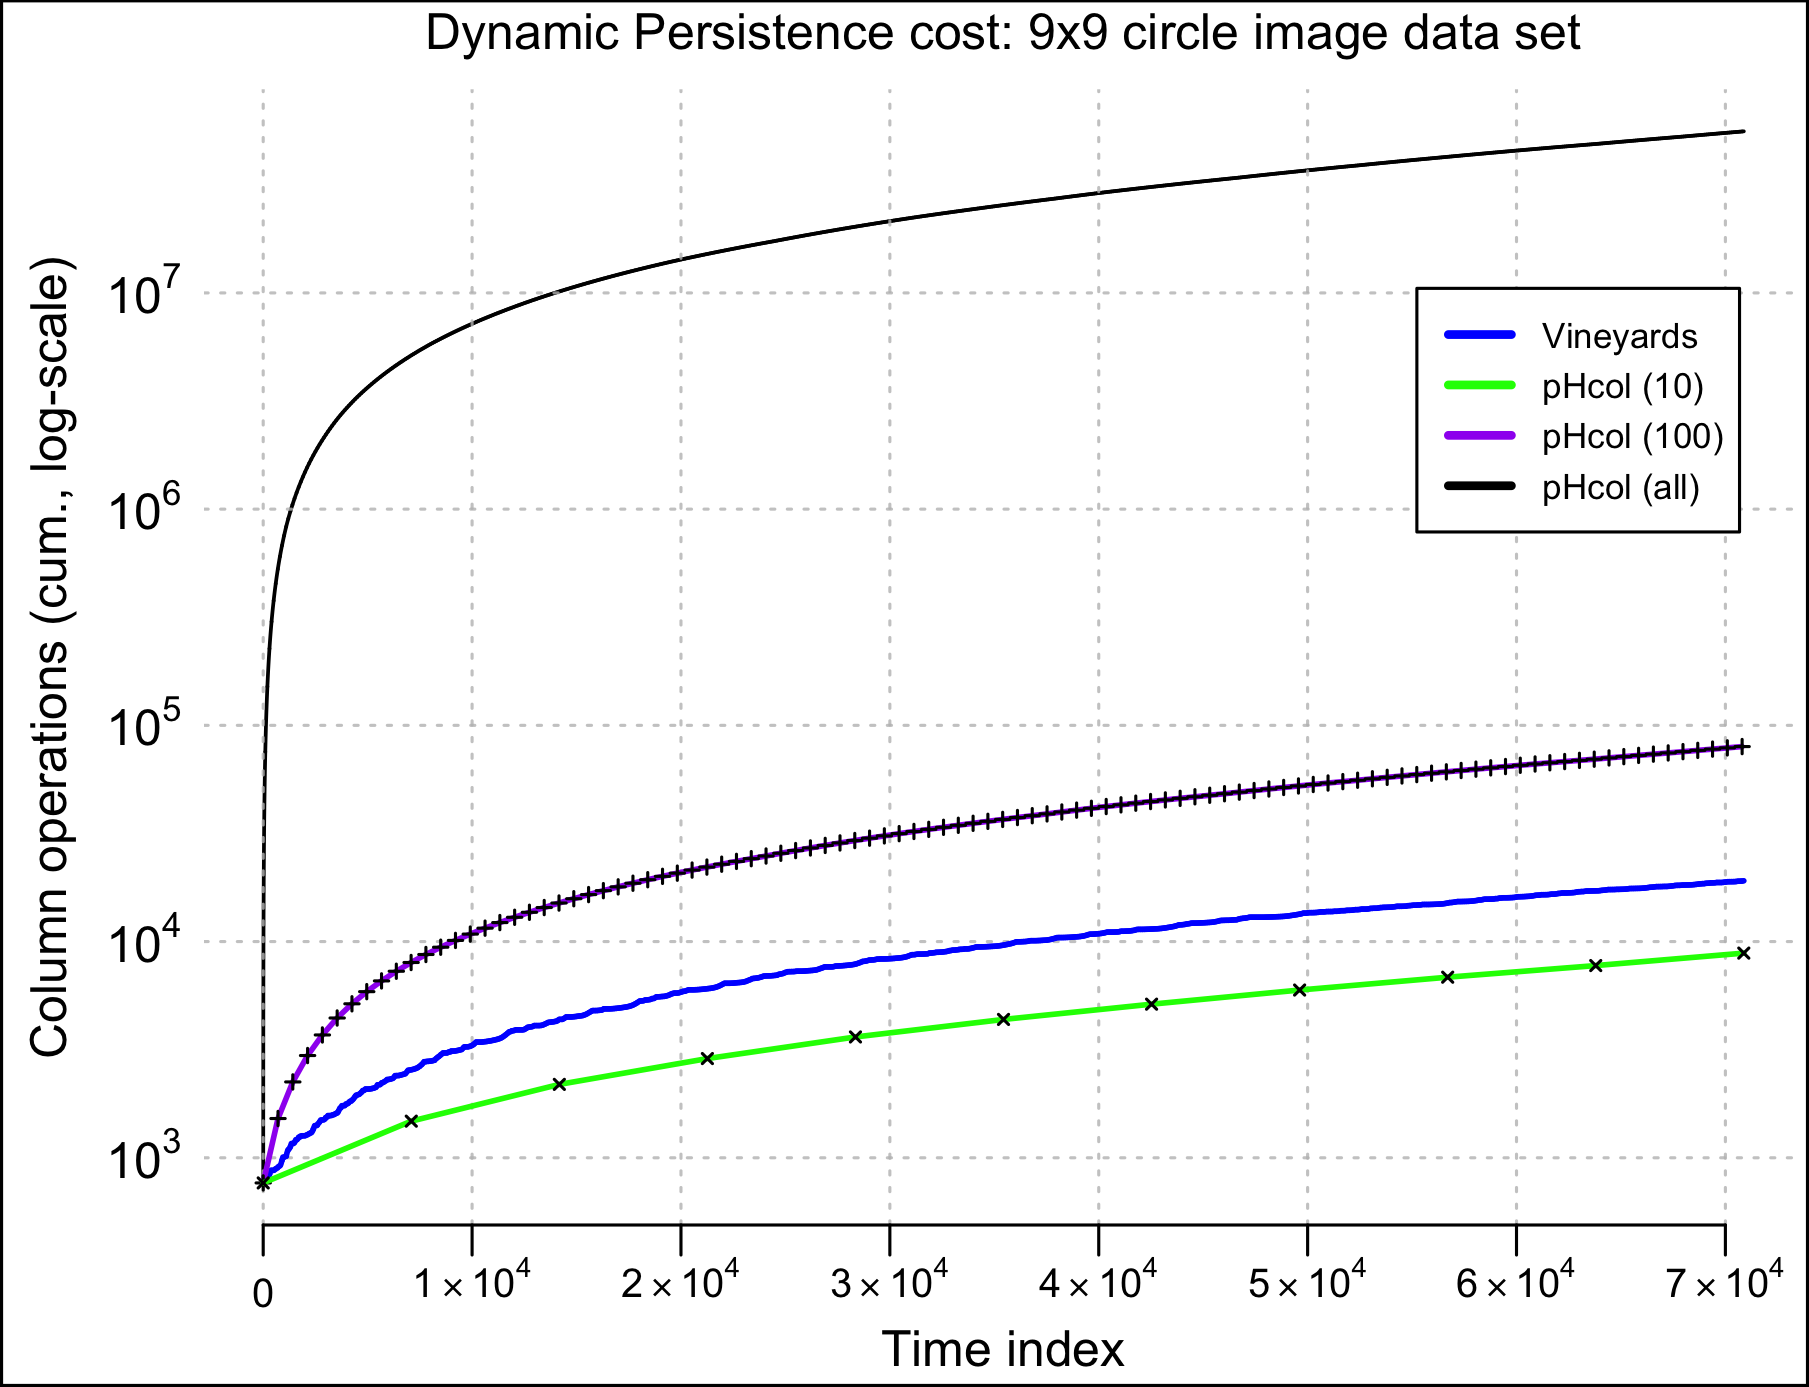
\includegraphics[width=0.36\textwidth, height = 1.45in]{circle_vineyards.png}
 	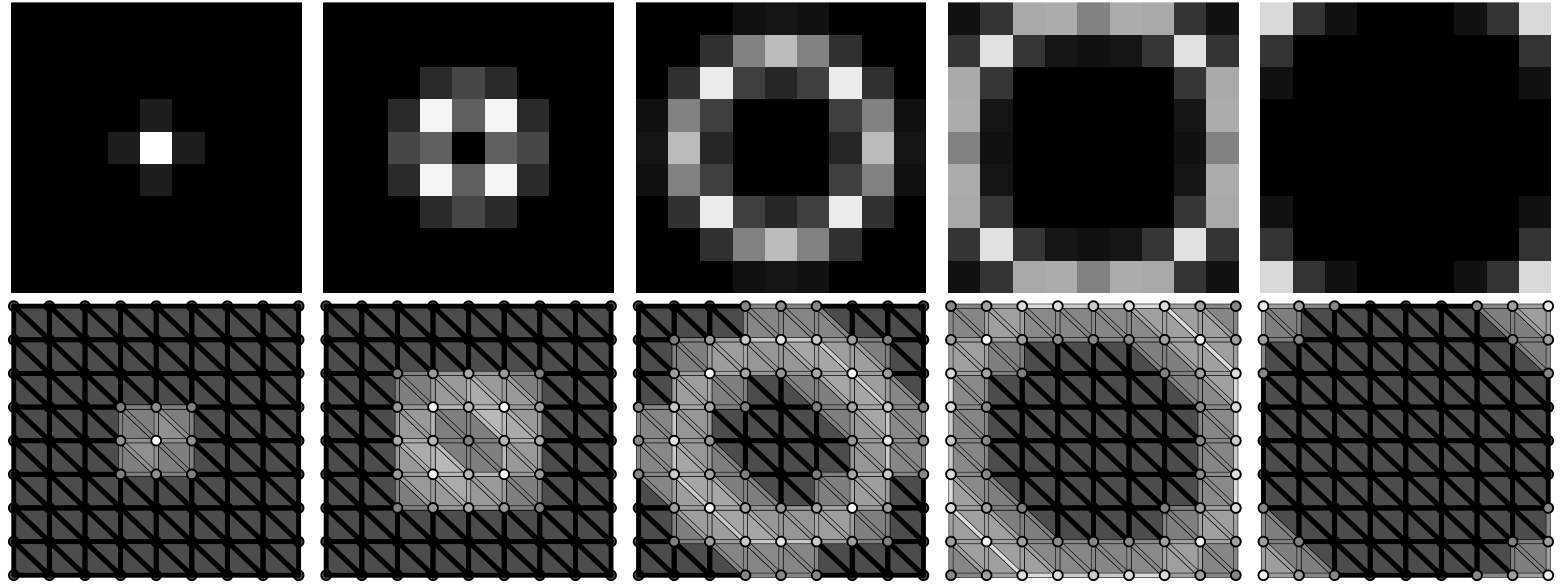
\includegraphics[width=0.63\textwidth, height = 1.45in]{circle_complex.png}
 	\caption{On the right, the grayscale image data set and corresponding lower star filtrations. On the left, the cumulative number of column operations required to compute persistence for this time-varying filtration. The   Betti numbers for each of the shown  steps in the filtration, from left to right, are: $(\beta_0,\beta_1, \beta_2)  = (1,0,0), \; (1,1,0),  \; (1,1,0), \; (1,1,0), \; (4,0,0)$. Observe that computing the diagrams independently at 10 evenly spaced time points (the green line) both captures these major topological changes and is the most computationally efficient approach shown.}
 	\label{fig:vineyards}
 \end{figure*}
Snapshots of the image data and its corresponding time-varying filtration is depicted in Figure~\ref{fig:vineyards} (top right and bottom right, respectively), which we use as a baseline for comparing vineyards and the standard reduction algorithm $\texttt{pHcol}$ (Algorithm \ref{alg:reduce}).
Note that the size of the filtration is fixed---no simplices are ever added or removed over time. 
There are two events which dramatically alter the persistence diagrams extracted from these filtrations: the first occurs when the central connected component splits to form a cycle, and the second  when the annulus  splits into four components. As a consequence, in this example, only a few persistence diagrams are needed to capture the major topological changes over time. 
  
  Consider the situation where one is concerned with capturing these dramatic changes in homology.
  On the left side of Figure~\ref{fig:vineyards}, we compare the cumulative cost (in total number of column operations) of various approaches.
  Since it is unknown a priori at which times  the persistent homology will change, one solution is to discretize the time domain at $n$ evenly spaced points and compute the persistence diagrams at each one of them  independently. 
  An alternative approach is to construct a (e.g., straight-line) homotopy between  contiguous time-points, and then decompose these homotopies into adjacent transpositions in the filtration order---the vineyards approach. The former is often used in practice, but it is only an approximation; the latter is guaranteed to capture all homological changes in persistence that occur in simulating the 1-parameter family. 
  The graph in Figure~\ref{fig:vineyards} depicts two different size approximations (purple, $n=100$ and green, $n=10$), wherein the reduction algorithm (\texttt{pHcol}) was applied at $n$ time points, and two exact strategies (black and blue), which compute all $\approx 7 \times 10^{4}$ diagrams given by the homotopy. 
  As shown in the figure, if one needs to simulate the homotopy exactly, then the vineyards approach is indeed far more efficient than naively applying the reduction algorithm independently at all time points.
  However, when the discretization of the time domain is coarse enough, the naive approach actually performs less column operations than the vineyards strategy, while still capturing the main events. 
  
  The existence of a time discretization that is more efficient to compute than continually updating the decomposition, indicates that the vineyards algorithm must incur some overhead (in terms of column operations) to perform transpositions, even if the persistence diagrams remain unchanged. 
  Even in situations where one is updating a decomposition to a filtration that is  relatively ``close''---e.g. any two adjacent filtrations in the bottom right of Figure~\ref{fig:vineyards}---it is still more efficient to apply \texttt{pHcol} directly than  to iteratively update the decomposition (see the case where $n = 10$). 
 Moreover, any optimization to the reduction algorithm (e.g.,  clearing~\cite{chen2011persistent}) would only increase this disparity.
 See~\cite{topaz2015topological, xian2020capturing, lesnick2015interactive, kim2020spatiotemporal} 
 for relevant scenarios and applications. 
 
\textbf{Our approach and contributions are as follows:} First, we leverage the \emph{moves} framework of Busaryev et. al.~\cite{busaryev2010tracking} to include  coarser  operations---in terms of the number of valid intermediate decomposition states, as compared to vineyards---for dynamic persistence. 
We give a tight lower bound on the number of moves needed to perform an arbitrary permutation to the $R = D V$ decomposition, and give a proof of optimality by a reduction to the permutation edit distance problem.
We also give worst-case bounds in expectation as well as efficient algorithms for achieving these bounds---both of which are derived from a reduction to the Longest Increasing Subsequence (LIS) problem. 
This reduction yields an efficient algorithm for generating sequences of moves $( s_1, s_2, \dots, s_d )$ of minimal size $d$, which we call \emph{schedules}. 
However, not all minimal size schedules incur the same  cost 
(i.e., number of column operations).
We investigate the feasibility of choosing optimal cost schedules, and show that 
greedy-type approaches can lead to arbitrarily bad behavior. 
In light of these results, we give an alternative proxy-objective for cost minimization, provide bounds justifying its relevance to the original problem, and give an efficient $O(d^2 \log m)$ algorithm for approximately solving this proxy minimization. 
A performance comparison with other reduction-based persistent homology computations is given; 
our move schedules are demonstrated to be an order of magnitude more efficient than existing approaches in applications such as flock simulations and 2D persistence computations with RIVET. 
%We conclude with a discussion of situations where our strategy is most applicable and future directions for research.  
   
\subsection{Related Work}\label{sec:related_work} 
To the authors knowledge, work focused on ways of updating a  decomposition $R = DV$, for all homological dimensions, is limited---there is the vineyards algorithm~\cite{cohen2006vines} and the moves algorithm~\cite{busaryev2010tracking}, both of which are discussed extensively in section~\ref{sec:background}. 

In contrast, there is extensive work  on improving the efficiency of computing a (static) $R = DV$ decomposition. Chen~\cite{chen2011persistent} proposed \emph{persistence with a twist}, also called the \emph{clearing optimization}, which exploits a boundary/cycle relationship to ``kill'' columns early in the reduction rather than reducing them. 
Another popular optimization is to utilize the duality between   homology and cohomology~\cite{de2011dualities}, which dramatically improves the effectiveness of the clearing optimization~\cite{bauer2021ripser}. 
There are many other optimizations on the implementation side: the use of ranking functions defined on the combinatorial number system enables implicit cofacet enumeration, removing the need to store the boundary matrix explicitly; the apparent/emergent pairs optimization identifies columns whose pivot entries are unaffected by the reduction algorithm, reducing the total number of columns which need be reduced; sparse data structures such as bit-trees and lazy heaps allow for efficient column-wise additions with $\mathbb{Z}_2 = \mathbb{Z}/2\mathbb{Z}$ coefficients and effective $O(1)$ pivot entry retrieval, and so on~\cite{bauer2021ripser, bauer2017phat}. 

By making stronger assumptions on the underlying topological space, restricting the homological dimension, or targeting  a weaker invariant (e.g. Betti numbers), one can usually obtain  faster or alternative approaches  recording information related to persistence.
For example, Attali et al.~\cite{attali2009persistence} give a linear time algorithm (under the $\texttt{word RAM}$ model of computation) for computing persistence on graphs.
In the same paper, they describe how to obtain $\epsilon$-simplifications of $1$-dimensional persistence diagrams for filtered $2$-manifolds by using duality and symmetry theorems. 
Along a similar vein, Edelsbrunner et. al.~\cite{edelsbrunner2000topological} give a fast incremental algorithm for computing persistent Betti numbers up to dimension $2$, again by utilizing symmetry, duality, and ``time-reversal''~\cite{delfinado1995incremental}. Chen et. al.~\cite{chen2013output} give an output-sensitive method for computing persistent homology,  utilizing the property that certain submatrices of  $D$ have the same rank as  $R$, which they exploit through fast sub-quadratic sparse-matrix rank algorithms.  

If  zeroth homology is the only dimension of interest, computing and updating both the persistence and rank information  is greatly simplified. For example, if the relations are available a-priori, obtaining a tree representation fully characterizing the connectivity of the underlying space (also known as the \emph{incremental connectivity} problem) takes just $O(\alpha(n) n)$ time using the disjoint-set data structure, where $\alpha(n)$ is the extremely slow-growing inverse Ackermann function. 
Adapting this approach to the time-varying setting, Oesterling et al.~\cite{oesterling2015computing} give a $O(e)$-per-update algorithm that allows one to maintain a \emph{merge tree} with $e$ edges,
associated to the filtration parameter changing continuously over time. 
If only the zeroth-dimensional Betti numbers are needed for a particular application, this problem reduces even further to tracking the connected components of a dynamic graph---sometimes referred to as the \emph{dynamic connectivity problem}, which can be efficiently  solved in amortized $O(\log n)$ query and update times using either Link-cut trees or multi-level Euler tour trees~\cite{kapron2013dynamic}.

\subsection{Outline} The remainder of the paper is organized as follows: we review and establish the notations we will use to describe simplicial complexes, persistent homology, and dynamic persistence in Section \ref{sec:background}. 
We also cover the reduction algorithm (designated here as \texttt{pHcol}), the vineyards algorithm, and the set of \emph{move}-related algorithms introduced in~\cite{busaryev2010tracking}, which serves as the starting point of this work. 
In Section \ref{sec:move_schedules} we introduce our move schedules  and provide efficient algorithms to make this alternative viable. 
In Section \ref{sec:results} we present applications of the proposed method. 
In particular, to the computation of crocker stacks from flock simulations, and to 2-dimensional persistence on the Mumford data set of image patches from natural images. 
In Section \ref{sec:conclusion} we conclude the paper by discussing other possible applications and future work. 
We also include an appendix which introduces certain topics in more detail, such as the vineyards algorithm itself, for readers who may be unfamiliar but would like a more in-depth understanding.


%\section*{Outline}
%\begin{outline}[enumerate]
%   \1 Background
%      \2 Point A1
%      \2 Point A2
%         \3 ...
%            \4 ...
%   \1 Point B
%      \2 Point B1
%         \3 Point B1a
%            \4 ...
%\end{outline}
% Interesting+ hard + solved + novel. 

\section{Background}\label{sec:background} 
\subsection{Notation}\label{sec:notation} 

Suppose one has a family $\{K_i\}_{i\in I}$ of simplicial complexes indexed by a totally ordered   set $I$, and so that for any $i< j \in I$ we have $K_i \subseteq K_j$. There are two index sets of interest in what follows: $\mathbb{R}$ and $[n] = \{ 1, \dots, n\}$. 
Such a family is called a \emph{filtration},
which is deemed to be \emph{essential} if $i \neq j$ implies $K_i \neq K_j$.
Moreover, an essential filtration is said to be  \emph{simplexwise} if $K_j \smallsetminus K_i = \{\sigma_j\}$ 
whenever $j$ is the immediate successor of $i$ in $I$.
Any finite filtration may be trivially converted into an essential, simplexwise filtration via a set of \emph{condensing}, \emph{refining}, and \emph{reindexing} maps (see~\cite{bauer2021ripser} for more details). 
As a result, and without loss of generality, here we exclusively consider essential simplexwise filtrations. For brevity, we will simply refer to them as filtrations. 

Let $K$ be an abstract simplicial complex and $\mathbb{F}$ a field.
A $p$-chain is a
formal $\mathbb{F}$-linear combination  of $p$-simplices of $K$. The collection of $p$-chains under addition yields an 
$\mathbb{F}$-vector space  denoted   $C_p(K)$. 
The $p$-boundary $\partial_p(\sigma)$  of a $p$-simplex $\sigma\in K$ is the alternating sum of its oriented co-dimension 1 faces,
and the $p$-boundary of a $p$-chain is defined 
linearly in terms of its constitutive simplices. 
A $p$-chain with zero boundary is called a $p$-cycle, and together they form $Z_p(K) = \mathrm{Ker}\,\partial_p$. 
Similarly, the collection of $p$-boundaries forms  $B_p(K) = \mathrm{Im}\,\partial_{p+1}$.
Since $\partial_p \circ \partial_{p+1} = 0$ for all $p\geq 0$, 
then the quotient space $H_p(K) = Z_p(K) / B_{p}(K)$ is well-defined, and called the 
$p$-th homology of $K$ with coefficients in $\mathbb{F}$. 
If $\{K_i\}_{i\in [m]}$ is a filtration, then the inclusion maps  $K_i\subset K_{i+1}$   induce linear transformations 
%$f_p^{i,j}: H_p(K_i) \to H_p(K_j)$ 
at the level of homology:
\begin{equation}
	H_p(K_1) \to H_p(K_2) \to \dots \to H_p(K_m)
\end{equation}
%The $p$-th persistent homology groups are the images of these transformations: $H_{p}^{i,j} = \mathrm{Im}\,f_p^{i,j}$. 
%Note that if $i = j$, then $H_{p}^{i,j} = H_{p}(K_i) = H_{p}(K_i)$ is   just the ``standard'' homology. 
Simplices whose inclusion in the filtration creates a new homology class are   called \emph{creators}, and simplices that destroy homology classes are   called \emph{destroyers}. 
The filtration indices of 
these creators/destroyers are referred to as \emph{birth} and \emph{death} times, respectively. 
The collection of birth/death  pairs 
$(i,j)$ is denoted $\mathrm{dgm}_p(K)$, 
and referred to as the $p$-th \emph{persistence diagram} of $K$.
If a homology class is born at time $i$ and dies entering time $j$, the difference $\lvert i - j \rvert$ is called the \emph{persistence} of that class.
In practice, filtrations often arise from triangulations parameterized by geometric scaling parameters, and the ``persistence'' of a homology class actually refers to its lifetime with respect to the scaling parameter. 
%For this reason, we'll refer to the difference $\lvert i - j \rvert$ of a homology class $[c]$ as its \emph{index persistence}.
\\
\\
\noindent \textbf{Example 2.1:} Non-essential filtrations often arise in geometrical contexts. For example, given a finite metric space $(X, d)$, the \emph{Vietoris-Rips} complex at scale $\epsilon \in \mathbb{R}$ is the abstract simplicial complex given by: 
\begin{equation}\label{eq:rips}
	\mathrm{Rips_\epsilon}(X) = \{ S \subseteq X : S \neq \emptyset \;\mbox{ and }\;\mathrm{diam}(S) \leq \epsilon \}
\end{equation} 
The corresponding filtration is called the \emph{Vietoris-Rips} (VR) filtration, indexed by $I = \mathbb{R}$. 
A VR filtration indexed over $\mathbb{R}$  can be condensed to an essential filtration indexed over the set of pairwise distances $\{\, d(x,x') \; | \; x,x' \in X \, \}$, 
which can then be further reindexed to an essential simplexwise filtration by extending a total order of $X$ to its power set---e.g., 
using the lexicographical ordering. 
%This is often necessary in the computational setting, where it is easier to work with a filtration with $m$ simplices indexed over $[m]$ instead of $\mathbb{R}$. 
\\
\\
Let $\mathbb{X}$ be a triangulable topological space. 
That is, so that there exists an abstract 
simplicial complex $K$ whose geometric realization  is homeomorphic to 
$\mathbb{X}$. 
Let  $f: \mathbb{X} \to \mathbb{R}$ be continuous and  
write $\mathbb{X}_a = f^{-1}(-\infty, a]$ to denote the sublevel sets of $\mathbb{X}$ defined by the value $a$. 
A \emph{homological critical value} of $f$ is any value $a \in \mathbb{R}$ such that the homology of the sublevel sets of $f$ changes at $a$, i.e.  if for some $p$ the inclusion-induced homomorphism  $H_p(\mathbb{X}_{a - \epsilon}) \to H_p(\mathbb{X}_{a+\epsilon})$ is not an isomorphism for  any small enough $\epsilon >0$. If there are only finitely many of these homological critical values, then $f$ is said to be \emph{tame}. 

Consider a homotopy $F(x,\tau) : \mathbb{X} \times [0,1] \to \mathbb{R}$ and denote its ``snapshot'' at a given time-point $\tau$ by $f_\tau(x) = F(x,\tau)$.
The snapshot $f_0$ denotes the initial function at time $\tau = 0$ and $f_1$ denotes the function at the last time step. 
As $\tau$ varies in $[0,1]$, the points in $\mathrm{dgm}_p(f_\tau)$ trace  curves in $\mathbb{R}^3$, called \emph{vines} and which together form a \emph{vineyard}. 
The stability of persistence implies that these curves will be continuous if $F$ is continuous
and the $f_\tau$'s are tame \cite{cohen2007stability}.
The vineyard analogy acts as a guidepost for practitioners seeking to understand how subtle changes occurring to the topological structure over time.
A more detailed discussion of the vineyards approach is provided in section~\ref{sec:vineyards}.
%Let $\mathbb{M}$ be a smooth $d$-manifold and $f : \mathbb{M} \to \mathbb{R}$ a smooth function. 
%A critical point $x$ is called \emph{non-degenerate} if the Hessian matrix of second partial derivatives is non-singular, otherwise if the Hessian is zero $x$ is said to be \emph{degenerate}. A \emph{Morse function} is a smooth function that has only non-degenerate critical points with distinct critical values. 
%and two Morse functions $f_0, f_1: \mathbb{M} \to \mathbb{R}$, and further suppose we equip $f_0, f_1$ with with a smooth homotopy $F : \mathbb{M}: [0,1] \to \mathbb{R}$ such that $F(x, 0) = f_0(x)$ and $F(x, 1) = f_1(x)$ for $x \in \mathbb{M}$. We use $f_\tau$ to denote the function at $F(x, \tau)$, where $\tau \in [0, 1]$. 
\subsection{The Reduction Algorithm}\label{sec:reduction}
In this section we briefly recount the original reduction algorithm introduced in~\cite{zomorodian2005computing}, also sometimes called the \emph{standard} algorithm or more explicitly \texttt{pHcol}~\cite{de2011dualities}. 
The pseudocode is outlined in Algorithm~\ref{alg:reduce}. Without optimizations, like   clearing   or       implicit matrix reduction, the standard  algorithm is very inefficient. Nonetheless, it serves as the foundation of most implementations that compute persistent homology, and its invariants are necessary before introducing both vineyards in section~\ref{sec:vineyards} and our move schedules  in section~\ref{sec:move_schedules}.

\begin{algorithm}[t]
	\setstretch{1.15}
	\caption{Reduction Algorithm (\texttt{pHcol}) }
	\begin{algorithmic}[1]
		\Require{$D = (m \times m)$ filtration boundary matrix }
		\Ensure{$R$ is reduced, $V$ is full rank upper triangular, and $R = D V$}
		\Function{Reduction}{$D$}
		\State $(R, V) \gets (D, I)$
		\For{$j = 1$ \textbf{to} $m$} 
			\While{$\exists \, i < j$ \textbf{such that} $\mathrm{low}_R(i) = \mathrm{low}_R(j)$ }
				\State $\lambda \gets \mathrm{pivot}_R(j)/\mathrm{pivot}_R(i)$
				\State $(\mathrm{col}_R(j), \mathrm{col}_V(j)) \mathrel{-}= \left ( \lambda \cdot \mathrm{col}_R(i), \lambda \cdot \mathrm{col}_V(i) \right )$
			\EndWhile
		\EndFor 
		\State \Return $(R, V)$
		\EndFunction
	\end{algorithmic}	\label{alg:reduce}
\end{algorithm}

 The main output of the reduction algorithm is a matrix decomposition $R = D V$, where the persistence diagram is encoded in $R$, and the generating cycles in the columns of $V$. 
 Given a  filtration $K$ with $m$ simplices and maximal dimension $d$, 
 one assembles the elementary boundary chains $\partial(\sigma)$ as columns ordered according to the filtration, forming the \emph{filtration boundary matrix} $D$. 
 The reduction algorithm can  compute the persistent homology for all dimensions up to $d - 1$.
 In this case,  $D$ is a square matrix of size $m \times m$. Alternatively, a single dimension $i \leq d - 1$ can be computed, in which case one reduces a pair of sub-matrices  $D_i$ and $ D_{i+1}$ of $D$,  where $D_i$ has dimension $d_{i-1} \times d_i$ and $D_{i+1}$ is  $d_{i} \times d_{i+1}$. 
 If one is interested in a particular dimension of homology, then the latter approach is preferred. However, the  description of the algorithms is simpler when considering the full matrix, so $D$ will always be $(m \times m)$ in what follows. 
 All algorithms discussed generalize to both situations. We give an example using the matrix pair $(R_1, V_1)$  below. 
\\
\\
\noindent
\textbf{Example 2.1: Reduction} Consider a triangle with vertices $u,v,w$, edges $a = (u,w)$, $b = (v,w)$, $c = (u, v)$,
and whose filtration order, read as inclusions from left to right, is given as $K = (u, v, w, a, b, c)$. The reduction algorithm begins by setting $R = D$ and $V = I$, followed by left-to-right column operations until invariant I2 below is satisfied.
If the $i$-th column of $R$ is nonzero, then $\mathrm{low}_R(i)$ 
is the row index of its lowest nonzero entry.
Using $\mathbb{Z}_2$ coefficients and homology in dimension 1 to simplify the presentation, the reduction proceeds as follows:
\begin{displaymath}
	\def\rowsp{0.4em}
	\def\arraystretch{0.95}
	\makeatletter\setlength\BA@colsep{1.2pt}\makeatother
	%
	\begin{blockarray}{cccc}{R_1}
	 \kern-0.2em & a & b & c  \\
		\begin{block}{c[ccc]}
  		u \kern\rowsp  & \; 1 &    &  1 \; \topstrut \\
  		v \kern\rowsp & \;     &  1 & 1 \; \\
  		w \kern\rowsp & \; 1 &  \fbox{1} &    \; \botstrut \\
		\end{block}
	\end{blockarray}
	\; , \;
	\begin{blockarray}{cccc}{V_1}
	\kern-0.2em & a & b & c  \\
		\begin{block}{c[ccc]}
        a \kern\rowsp  & \; 1 &  &  \; \topstrut \\
  		b \kern\rowsp & \;  & 1 & \; \\
  		c \kern\rowsp & \;  &  & 1 \; \botstrut \\
		\end{block}
	\end{blockarray}
	\quad \xrightarrow{} \,
	\begin{blockarray}{cccc}{R_1}
	\kern-0.2em & a & b & c  \\
		\begin{block}{c[ccc]}
  		u \kern\rowsp  & \; 1 & 1 & 1 \; \topstrut \\
  		v \kern\rowsp & \;     & 1 & \fbox{1} \; \\
  		w \kern\rowsp & \; 1 &    &    \; \botstrut \\
		\end{block}
	\end{blockarray}
	\; , \;
	\begin{blockarray}{cccc}{V_1}
	\kern-0.2em & a & b & c  \\
		\begin{block}{c[ccc]}
  		a \kern\rowsp  & \; 1 & 1 &    \; \topstrut \\
  		b \kern\rowsp & \;     & 1 &    \; \\
  		c \kern\rowsp & \;     &    & 1 \; \botstrut \\
		\end{block}
	\end{blockarray}
	\quad \xrightarrow{} \,
	\begin{blockarray}{cccc}{R_1}
	\kern-0.2em & a & b & c  \\
		\begin{block}{c[ccc]}
  		u \kern\rowsp  & \; 1    & 1  &  \; \topstrut \\
  		v \kern\rowsp &  \;    & 1  &  \; \\
  		w \kern\rowsp & \; 1  &     &  \; \botstrut \\
		\end{block}
	\end{blockarray}
	\; , \;
	\begin{blockarray}{cccc}{V_1}
	\kern-0.2em & a & b & c  \\
		\begin{block}{c[ccc]}
  		b \kern\rowsp  & \; 1 & 1 & 1 \; \topstrut \\
  		a \kern\rowsp & \;     & 1 & 1 \; \\
  		c \kern\rowsp & \;     &    & 1 \; \botstrut \\
		\end{block}
	\end{blockarray}
	\vspace*{-1em}
\end{displaymath}
\noindent The column $c$ in $R$ indicates that dimension $1$ homology is born, which in this filtration is never killed since the dimension of the complex is $1$. Similarly, the columns at $u, v, w$ in $R_0$ (not shown) are all zero, indicating three $0$-dimensional homology classes  are born, which are then killed by the pivot entries in columns $a$ and $b$ in $R_1$.
\\
\\
\noindent
It is clear from Algorithm~\ref{alg:reduce} that a loose upper bound for this reduction is $O(m^3)$, where $m$ is the number of simplices of the filtration; it turns out that this bound is in fact tight, see~\cite{morozov2005persistence} for more details. 
There are actually many variations and optimizations proposed over the past decade to Algorithm~\ref{alg:reduce}; for example, one can   reverse the order of the filtration and compute cohomology~\cite{de2011dualities} instead. Despite these variations in computation, regardless of how the decomposition is obtained, it must obey the following invariants:
  \vspace*{0.8em}
 \begin{enumerate}[leftmargin=2\parindent, align=left, labelsep=-5pt, topsep=0pt,itemsep=-0.25ex,parsep=1.2ex]
	\item[\hspace{-1.5em}\textbf{ Decomposition Invariants:}]
 	\item[I1] $R = D V$ where $D$ is the boundary matrix of the filtration $K$
 	\item[I2] $V$ is full-rank upper-triangular, and $R$ is \emph{reduced}: if its $i$-th and $j$-th columns are nonzero, then $\mathrm{low}_R(i) \neq \mathrm{low}_R(j)$ 
 	\end{enumerate} 
 \vspace*{1em}
 If these two invariants are satisfied, then we call the decomposition \emph{valid}. Given any valid $R = D V$ decomposition, then~\cite{zomorodian2005computing}:
%\begin{proposition}[Persistent Pairing~\cite{zomorodian2005computing}]
%	Let $R = D V$, where $R$ is in reduced form and $V$ is full-rank upper triangular (invariants (1) and (2)  hold). Then the pairing $(\sigma_i, \sigma_j)$ defined by $i = \mathrm{low}_R(j)$ is a \emph{creator/destroyer (persistent) pair}. While the matrices $R,V$ satisfying (1) and (2) are not unique in general,  the persistent pairs $(i,j)$ are unique and define the persistence diagrams of $K$.
%\end{proposition}
\noindent
The collection of persistent pairings is independent of the choice of $R$ and $V$. When reducing the boundary matrix, we can therefore perform column operations in any order, as long as columns are added from left to right, and so long as every column operation performed in $R$ is also performed on $V$. 
Once $R$ is reduced, then the low entries in $R$ yield the correct pairings encoding the persistence diagram of the corresponding filtration $K$.
% Important corollaries of the persistence pairing lemma is that the 
% The pairing given by the lowest non-zero entries of $R$ is uniqueness, even thought the decomposition itself not.  
% \section*{Computational Perspective} To convey a meaningful computational perspective, the continuous notion of \emph{dynamic persistence} needs to be translated to a discrete, combinatorial definition. Such a description requires a few prerequisite definitions, accompanied by some simplifying assumptions. 
%\subsection*{A General Matrix Framework} Perhaps the most frequently used approach to computing the persistence diagram of a given filtration $K$ is with the \emph{reduction} algorithm. There have been many advancements in the past decade in improving the reduction algorithm---a comprehensive overview is beyond the scope of this effort. The majority of these computational improvements were developed to improve the efficiency of performing the \emph{initial} reduction. A concise summary of these advancements can be found in~\cite{bauer2019ripser}. In contrast, we focus here on improving the efficiency of maintaining a \emph{given} decomposition under an arbitrary reordering.  
\subsection{Vineyards}\label{sec:vineyards}
The original purpose of the vineyards algorithm, as described in~\cite{cohen2006vines}, was to compute a continuous 1-parameter family of persistence diagrams over a time-varying filtration, and to detect homological critical events during the construction.
Notice that homological critical events can only occur when the filtration order changes, though the converse is not true.
Thus, detecting  all such events reduces to computing matrix decompositions at a finite set of time points interleaved between changes in the filtration order. 
At the finest scale, these changes manifest as transpositions of adjacent simplices. 
As a result, a fixed set of rules for maintaining a valid $R = D V$ decomposition under adjacent transpositions  is enough to simulate persistence dynamically. 
These rules prescribe certain column and row operations which must be applied to the matrix decomposition either before, during, or after the transposition, in order to ensure decomposition invariants I1 and I2 are respected.   

Let $S_{i}^j$ represent the upper-triangular matrix such that multiplying by it on the right is equivalent to adding column $i$ to column $j$. 
Multiplication by $S_{i}^j$ on the left is equivalent to adding row $j$ to row $i$.
% NOT SURE about this:, and thus $S_{i}^j S_{i}^j = I$. 
Similarly, let $P$ denote the matrix so that multiplication from the right applies a fixed permutation to the columns of $A$.
Since the columns of $P$ are orthonormal, then  $P^{-1} = P^T$, and thus one would write $P^T A P$ to denote the application of the same permutation  to both the columns and rows of $A$. In the special case where $P$ represents a transposition, we have $P = P^T$ and may instead simply write $P A P$. 
The goal of the vineyards algorithm can now be described explicitly: to prescribe a set of rules, written as matrices $S_{i}^{j}$, such that if $R = D V$ is a valid decomposition, then $(\ast P \ast R \ast P \ast) = (PDP)(\ast P\ast V \ast P \ast)$ is also a valid decomposition, where $\ast$ is some number (possibly zero) of matrices encoding elementary column or row operations. 
%We refer to the algorithm that maintains the $R = \partial V$ decomposition under adjacent permutations $P$ as the \emph{transposition framework}. 
% The explicit pseudocode describing these rules is given in the appendix by Algorithm~\ref{alg:tr}. 
%	\; = 
%	\begin{blockarray}{cccc}
%	\tiny{D_1} \kern-0.2em & a & b & c  \\
%		\begin{block}{c[ccc]}
%  		u \kern-0.1em & \; 1 & 1 & 0 \; \topstrut \\
%  		v \kern-0.1em & \; 0 & 1 & 0 \; \\
%  		w \kern-0.1em & \; 1 & 0 & 0 \; \botstrut \\
%		\end{block}
%	\end{blockarray}	
%	\;\, 
%	+
\\
\\
\noindent 
\textbf{Example 2.2} To illustrate the basic principles on which vineyards works, we re-use the running example introduced in the previous section. Below, we illustrate the case of exchanging simplices $a$ and $b$ in the filtration order, and restoring $RV$ to a valid decomposition. 
\begin{displaymath}
	\def\rowsp{0.4em}
	\def\arraystretch{0.95}
	\makeatletter\setlength\BA@colsep{1.2pt}\makeatother
	%
	\begin{blockarray}{cccc}{R_1}
	 \kern-0.2em & a & b & c  \\
		\begin{block}{c[ccc]}
  		u \kern\rowsp  & \; 1 & 1 &  \; \topstrut \\
  		v \kern\rowsp & \;  & 1 &  \; \\
  		w \kern\rowsp & \; 1 &  &  \; \botstrut \\  
		\end{block}
	\end{blockarray}
	\,\,, 
	\begin{blockarray}{cccc}{V_1}
	\kern-0.2em & a & b & c  \\
		\begin{block}{c[ccc]}
        a \kern\rowsp  & \; 1 &  \fbox{1} & 1 \; \topstrut \\
  		b \kern\rowsp & \;  & 1 & 1 \; \\
  		c \kern\rowsp & \;  &  & 1 \; \botstrut \\
		\end{block}
	\end{blockarray}
	\xrightarrow{S_{1}^2} 
	\hspace{-0.1em}
	\begin{blockarray}{cccc}{}
	\kern-0.2em & a & b & c  \\
		\begin{block}{c[ccc]}
  		 & \; 1 &  &  \; \topstrut \\
  		 & \;  & 1 &  \; \\
  		 & \; 1 & 1 & \; \botstrut \\
		\end{block}
	\end{blockarray}
	\,\,, 
	\begin{blockarray}{cccc}{}
	\kern-0.2em & a & b & c  \\
		\begin{block}{c[ccc]}
  		 & \; 1 &  & 1 \; \topstrut \\
  		 & \;  & 1 & 1 \; \\
  		 & \;  &  & 1 \; \botstrut \\
		\end{block}
	\end{blockarray}
	\xrightarrow{P}
	\hspace{-0.2em}
	\begin{blockarray}{cccc}{}
	\kern-0.2em & b & a & c  \\
		\begin{block}{c[ccc]}
  		& \;  & 1 &  \; \topstrut \\
  		& \; 1 &  &  \; \\
  		& \; 1 & \fbox{1} &  \; \botstrut \\
		\end{block}
	\end{blockarray}
	\,\,, 
	\begin{blockarray}{cccc}{}
	\kern-0.2em & b & a & c  \\
		\begin{block}{c[ccc]}
  		& \; 1 &  & 1 \; \topstrut \\
  		& \;  & 1 & 1 \; \\
  		& \;  &  & 1 \; \botstrut \\
		\end{block}
	\end{blockarray}
	\xrightarrow{S_1^2}
	\hspace{-0.1em}
	\begin{blockarray}{cccc}{}
	\kern-0.2em & b & a & c  \\
		\begin{block}{c[ccc]}
  		u \kern\rowsp  & \;  & 1 &  \; \topstrut \\
  		v \kern\rowsp & \; 1 & 1 &  \; \\
  		w \kern\rowsp & \; 1 &  &  \; \botstrut \\
		\end{block}
	\end{blockarray}
	\,\,,
	\begin{blockarray}{cccc}{}
	\kern-0.2em & b & a & c  \\
		\begin{block}{c[ccc]}
  		  & \; 1 & 1 & 1 \; \topstrut \\
  		 & \; & 1 & 1 \; \\
  		 & \;  &  & 1 \; \botstrut \\
		\end{block}
	\end{blockarray}
\end{displaymath}
%Prior to performing the exchange, observe that that the bold entry in $V_1$ would render $V_1$ non-upper triangular after the exchange. This entry is removed by a left-to-right column operation, given by applying the $S_1^{2}$ on the right to $R_1$ and $V_1$. After this operation, the permutation may be safely applied to $V_1$. In this case, both before and after the permutation, $R_1$ is rendered non-reduced, requiring another column operation to restore the decomposition to a valid state.
Starting with a valid reduction $R = DV$ and prior to performing the exchange, observe that that the highlighted entry in $V_1$ would render $V_1$ non-upper triangular after the exchange. This entry is removed by a left-to-right column operation, given by applying the $S_1^{2}$ on the right to $R_1$ and $V_1$. After this operation, the permutation may be safely applied to $V_1$. Both before and after the permutation $P$, $R_1$ is rendered non-reduced, requiring another column operation to restore the decomposition to a valid state.

 The time complexity of vineyards is determined entirely by the complexity of performing a single adjacent transposition.
 Informally, since column operations are the largest complexity operations needed and each column can have potentially $m$ entries, the complexity of vineyards is $O(m)$ per transposition. 
 However, there are a number of subtleties involved in this statement. 
 The first  is that both the $V$ and $R$ matrices tend to be quite sparse, and thus column and row operations rarely require $m$ operations---in fact, as a rule of thumb, most transpositions require no column operations~\cite{edelsbrunner2000topological}. A second subtlety, due to the necessity of sparse matrix data structures, is that querying the non-zero status of any particular entry typically takes $O(\log m)$ time. This hidden cost may seem minor, however, the quadratic scaling of the number of transpositions vineyards typically requires makes this cost non-trivial.   
In fact, achieving $O(m)$ complexity per transposition requires a special sparse matrix representation that allows swapping any two rows and columns in $O(1)$---see the appendix for more details and discussion. Finally, note the constant factor associated with the stated complexity: inspection of the individual cases of the algorihtm from~\cite{cohen2006vines} shows that there are at most two $O(m)$ operations, on both $R$ and $V$, that may be needed for any single transposition.
 
 % As a rule of thumb, due to the sparsity of both $R$ and $V$, most transpositions actually require no $O(m)$ operations. For example, exchanging two simplices of differing dimensions never requires column operations. A simple analysis given by Chen et al.~\cite{chen2013output} quantifies the order of magnitude we can expect the sparsity of these matrices to be.  

\subsection{Moves}\label{sec:moves} Busaryev et al.~\cite{busaryev2010tracking} introduced an algorithm which maintains an $R = D V$ decomposition under \emph{move operations}. A move operation $\mathrm{Move}(i,j)$ is a set of rules for maintaining a valid decomposition under the application of a permutation $P$ that moves a simplex $\sigma_i$ at position $i$ to position $j$. If $j = i \pm 1$, this operation is an adjacent transposition, and thus in some sense Busaryev's move algorithm is a generalization of  vineyards.

Though they are similar, move operations confer a few computational advantages compared to vineyards. Informally, a move operation has two convenient properties:
\\	
 \begin{enumerate}[leftmargin=2\parindent, align=left, labelsep=-5pt, topsep=0pt,itemsep=-0.25ex,parsep=1.2ex]
 	\item[M1:] Querying the non-zero status of entries in either $R$ or $V$ occurs once per move.
 	\item[M2:] $R = D V$ is \underline{not} guaranteed to be valid  during the movement of $\sigma_i $ to $ \sigma_j$.
 \end{enumerate} 
 \vspace*{1em}
First, consider property M1. Prior to applying any permutation $P$ to the decomposition, it is necessary to remove non-zero entries in $V$ which render $P^TVP$ non-upper triangular, to maintain invariant I2. 
If one uses the (augmented) sparse matrix representation described in~\cite{cohen2006vines}, checking whether these entries are non-zero takes $O(\log m)$ per column. Since moving a simplex from $i$ to $j$ using vineyards performs $\lvert i - j \rvert - 1$ transpositions, this query operation is required at most $O(\lvert i - j \rvert)$ times.
By comparison, if a row-oriented sparse matrix implementation is used, then a move operation can perform these non-zero entry checks in just one $O(m)$ pass, prior to performing any column operations. 

Property M2 indicates move operations only guarantee the decomposition is valid after the operation completes, implying that the decomposition is not fully maintained during the execution of \textit{RestoreRight} and \textit{RestoreLeft} below. 
This is a significant difference compared to the vineyards algorithm, which was designed specifically to maintain a valid decomposition after each transposition. 
In this way, we interpret move operations as making a tradeoff in granularity: whereas a sequence of adjacent transpositions $(i, i{+}1), (i{+}1, i{+}2), \dots, (j{-}1, j)$ generates $\lvert i - j \rvert $ valid decompositions in vineyards, a move operation $\mathrm{Move}(i,j)$ generates only one.
Indeed, if one has a pair of filtrations $(K_0, K_1)$ each with $m$ simplices, and we assume that each simplex $\sigma_i$ switches its relative ordering with another simplex $\sigma_j$ at most once in some ordered schedule of transpositions, then the number of intermediate persistence diagrams is bounded above by $O(m^2)$ using transpositions, whereas with move operations this bound clearly is at most $O(m)$.  \\ 

\noindent \textbf{Example:} We continue the example used in sections~\ref{sec:vineyards} and~\ref{sec:reduction} to illustrate moves. Consider moving the edge $a$ to the position of edge $c$ in the filtration. The donor columns introduced in~\cite{busaryev2010tracking} are shown on the left side of each matrix. Note that using vineyards, the equivalent permutation to the decomposition would require $4$ column operations on both $R_1$ and $V_1$, respectively, whereas a single move operation accomplishes this permutation using only $2$ column operations per matrix. 
\begin{displaymath}
	\def\rowsp{0.4em}
	\def\arraystretch{0.95}
	\makeatletter\setlength\BA@colsep{1.2pt}\makeatother
	%
	\begin{blockarray}{cc}{d_R}
	\kern-0.2em & a \\
		\begin{block}{c[c]}
  		u \kern \rowsp & \; 1 \; \topstrut \\
  		v \kern \rowsp & \;  \; \\
  		w \kern \rowsp & \; 1 \; \botstrut \\
		\end{block}
	\end{blockarray}
	\; \;
	\begin{blockarray}{cccc}{R_1}
	 \kern-0.2em & a & b & c  \\
		\begin{block}{c[ccc]}
  		u \kern \rowsp & \; 1 & 1 &  \; \topstrut \\
  		v \kern \rowsp & \;  & 1 &  \; \\
  		w \kern \rowsp & \; 1 &  &  \; \botstrut \\
		\end{block}
	\end{blockarray}
	%
\; \to
	%
\begin{blockarray}{cc}{}
	\kern-0.2em & b \\
		\begin{block}{c[c]}
  		  & \; 1 \; \topstrut \\
  		 & \;  1 \; \\
  		 & \; \; \botstrut \\
		\end{block}
	\end{blockarray}
	\; \;
\begin{blockarray}{cccc}{}
	\kern-0.2em & a & b & c  \\
		\begin{block}{c[ccc]}
  		  & \; 1 &    &  \; \topstrut \\
  		  & \;    & 1 &  \; \\
  		 & \; 1 & \fbox{1} &  \; \botstrut \\
		\end{block}
	\end{blockarray}
	%
\; \to
	%
	\begin{blockarray}{cc}{}
	\kern-0.2em & c \\
		\begin{block}{c[c]}
  		  & \; \hphantom{1} \; \topstrut \\
  		 & \;  \hphantom{1} \; \\
  		 & \; \hphantom{1} \; \botstrut \\
		\end{block}
	\end{blockarray}
	\; \; 
	\begin{blockarray}{cccc}{}
	\kern-0.2em & a & b &  c \\
		\begin{block}{c[ccc]}
  		  & \; 1   &    &   1  \; \topstrut \\
  		 & \;       &  1  &  1  \; \\
  		 & \; 1   &   \fbox{1}   &     \; \botstrut \\
		\end{block}
	\end{blockarray}
%
\; \xrightarrow{P} 
\begin{blockarray}{cc}{}
	\kern-0.2em & c \\
		\begin{block}{c[c]}
  		  & \; \hphantom{1} \; \topstrut \\
  		 & \; \hphantom{1} \; \\
  		 & \; \hphantom{1} \; \botstrut \\
		\end{block}
	\end{blockarray}
\; \;
\begin{blockarray}{cccc}{}
	\kern-0.2em & b & c & a  \\
		\begin{block}{c[ccc]}
  		  & \;  & 1 &  1\; \topstrut \\
  		 & \; 1 & 1 &  \; \\
  		 & \; 1 &  & \fbox{1} \; \botstrut \\
		\end{block}
	\end{blockarray}
%
\; \xrightarrow{d_R} 
\begin{blockarray}{cccc}{R_1}
\kern-0.2em & b & c & a  \\
	\begin{block}{c[ccc]}
		u \kern \rowsp & \;  & 1 &  \; \topstrut \\
		v \kern \rowsp & \; 1 & 1 &  \; \\
		w \kern \rowsp & \; 1 &  &  \; \botstrut \\
	\end{block}
	% \undermat{B}{ & & }  
\end{blockarray}
\end{displaymath}

\vspace{-1.0em}

% Start V example 
\begin{displaymath}
	\def\rowsp{0.4em}
	\def\arraystretch{0.95}
	\makeatletter\setlength\BA@colsep{1.2pt}\makeatother
	%
	\begin{blockarray}{cc}{d_V}
	\kern-0.2em & a \\
		\begin{block}{c[c]}
  		 & \; 1 \; \topstrut \\
  		& \;  \; \\
  		& \;  \; \botstrut \\
		\end{block}
	\end{blockarray}
	\; \;
	\begin{blockarray}{cccc}{V_1}
	 \kern-0.2em & a & b & c  \\
		\begin{block}{c[ccc]}
  		 & \; 1 & \fbox{1} &  \fbox{1}\; \topstrut \\
  		& \;  & 1 &  1\; \\
  		& \; &  & 1 \; \botstrut \\
		\end{block}
	\end{blockarray}
	%
\; \to
	%
\begin{blockarray}{cc}{}
	\kern-0.2em & b \\
		\begin{block}{c[c]}
  		 & \; 1 \; \topstrut \\
  		& \;  1 \; \\
  		& \; \; \botstrut \\
		\end{block}
	\end{blockarray}
	\; \;
\begin{blockarray}{cccc}{}
	 \kern-0.2em & a & b & c  \\
		\begin{block}{c[ccc]}
  		 & \; 1 & &  \fbox{1}\; \topstrut \\
  		& \;  & 1 &  1\; \\
  		& \; &   & 1 \; \botstrut \\
		\end{block}
	\end{blockarray}
	%
\; \to
	%
	\begin{blockarray}{cc}{}
	\kern-0.2em & c \\
		\begin{block}{c[c]}
  		 & \; 1 \; \topstrut \\
  		& \;  1 \; \\
  		& \; 1 \; \botstrut \\
		\end{block}
	\end{blockarray}
	\; \;
	\begin{blockarray}{cccc}{}
	\kern-0.2em & a & b &  c \\
		\begin{block}{c[ccc]}
  		 & \; 1 & &   \; \topstrut \\
  		& \;  & 1 &   \; \\
  		& \;  &   & 1 \; \botstrut \\
		\end{block}
	\end{blockarray}
%
\; \xrightarrow{P} \\
% 
\begin{blockarray}{cc}{}
	\kern-0.2em & a \\
		\begin{block}{c[c]}
  		 & \; 1 \; \topstrut \\
  		& \;  1 \; \\
  		& \; 1 \; \botstrut \\
		\end{block}
	\end{blockarray}
\; \;
\begin{blockarray}{cccc}{}
	\kern-0.2em & b & c & a  \\
		\begin{block}{c[ccc]}
  		 & \; 1 & &\; \topstrut \\
  		& \;  & 1 &  \; \\
  		& \; &  & 1 \; \botstrut \\
		\end{block}
	\end{blockarray}
%
\; \xrightarrow{d_V}
% 
	\begin{blockarray}{cccc}{V_1}
	\kern-0.2em & b & c & a  \\
		\begin{block}{c[ccc]}
  		b \kern \rowsp & \; 1 & & 1 \; \topstrut \\
  		c \kern \rowsp & \; & 1 &  1 \; \\
  		a \kern \rowsp & \; &  & 1  \; \botstrut \\
		\end{block}
	\end{blockarray}
\end{displaymath}

\begin{algorithm}[!htb]
	\caption{Move Right Algorithm}\label{alg:mr}
	\setstretch{1.15}
    \begin{algorithmic}[1]
        \Function{RestoreRight}{$R$, $V$, $\mathbb{I} = \{I_1, I_2, \dots, I_s \}$}
            \State $(\, d_{low}, \, d_R, \, d_V \,) \gets ( \, \mathrm{low}_R(I_1), \, \mathrm{col}_R(I_1), \, \mathrm{col}_V(I_1) \, )$
        	\For{$k$ \textbf{in} $I_2, \dots, I_s$} 
        		\State $( \, d_{low}', \, d_R', \, d_V' \, ) \gets ( \, \mathrm{low}_R(k), \, \mathrm{col}_R(k), \, \mathrm{col}_V(k) \, )$
        		\State $( \, \mathrm{col}_R(k), \, \mathrm{col}_V(k) \, ) \mathrel{+}= (\, d_R, \, d_V \,) $
        		\If {$d_{low}' < d_{low}$}
        			\State $(\, d_{low}, \, d_R, \, d_V \,) \gets (\, d_{low}', \, d_R', \, d_V' \, )$
        		\EndIf
        	\EndFor 
        	\State \Return $(\, R, \, V, \, d_R, \, d_V \, )$
        \EndFunction
    \end{algorithmic}
    \begin{algorithmic}[1]
        \Function{MoveRight}{$R$, $V$, $i$, $j$} 
            \State $\mathbb{I} =$ columns satisfying $V[i, i:j] \neq 0$ %\Comment{$O(m)$}
            \State $\mathbb{J} = $ columns satisfying $\mathrm{low}_R \in [i:j]$ and $\mathrm{row}_R(i) \neq 0$ %\Comment{$O(m)$}
            \State $(\, R, \, V, d_R, d_V \,) \gets $ \Call{RestoreRight}{$R$, $V$, $\mathbb{I}$} 
            %\Comment{Restores $p$-simplices} \Comment{$O(\lvert \mathbb{I} \rvert)$}
            \State $(\, R, \, V \,) \gets $ \Call{RestoreRight}{$R$, $V$, $\mathbb{J}$}
            	%\Comment{Restores $(p+1)$-simplices}
            	%\Comment{$O(m \lvert \mathbb{I} \rvert)$}
            \State $(\, R, \, V\, ) \gets (\, P R P^T, \, P V P^T\,)$  % \Comment{$P$ is a permutation given by (i,j)}
            \State $(\, \mathrm{col}_R(j), \, \mathrm{col}_V(j) \, ) \gets (\, P d_R, \, P d_V \,)$
            \State \Return $(\, R, \, V\,)$
        \EndFunction
    \end{algorithmic}
\end{algorithm}

\begin{algorithm}[!htb]
	\caption{Move Left Algorithm}\label{alg:ml}
	\setstretch{1.15}
    \begin{algorithmic}[1]
        \Function{RestoreLeft}{$R$, $V$, $\mathbb{K} = \{k_1, k_2, \dots, k_s \}$}
            % \State $\mathrm{low}_K \gets \{ \mathrm{low}_R(k_1), \mathrm{low}_R(k_2), \dots, \mathrm{low}_R(k_s) \}$
            \State $(l, r) \gets $ indices $l, r \in \mathbb{K}$ satisfying $l < r$, $\mathrm{low}_R(l) = \mathrm{low}_R(r)$ maximal 
            \While{$\mathrm{low}_R(l) \neq 0$ \textbf{and} $\mathrm{low}_R(r) \neq 0$}
            	\State $(\mathrm{col}_R(r), \mathrm{col}_V(r)) \mathrel{+}= (\mathrm{col}_R(l), \mathrm{col}_V(l))$
            	\State $\mathbb{K} \gets \mathbb{K} \setminus l$
            	\State $(l, r) \gets $ indices $l, r \in \mathbb{K}$ satisfying $l < r$, $\mathrm{low}_R(l) = \mathrm{low}_R(r)$ maximal
            \EndWhile
        	\State \Return $(\, R, \, V \, )$
        \EndFunction
    \end{algorithmic}
    
    \begin{algorithmic}[1]
        \Function{MoveLeft}{$R$, $V$, $i$, $j$} 
        	\State $\mathbb{J} \gets \{ j \}$
            % \State $(\mathbb{K}, d_R, d_V) \gets (\emptyset, \mathrm{col}_R(i), \mathrm{col}_V(i))$
            \While{$V(k, i) \neq 0 $\textbf{ for }$ k = \mathrm{low}_V(i)$\textbf{ where }$j \leq k < i$}
            	\State $(\mathrm{col}_R(i), \mathrm{col}_V(i)) \mathrel{+}= (\mathrm{col}_R(k), \mathrm{col}_V(k))$
            	\State $\mathbb{K} \gets \mathbb{K} \cup k + 1 $
            \EndWhile
            \State $(R, V) \gets (P R P^T, P V P^T)$
            \State $\mathbb{J} = $ columns satisfying $\mathrm{low}_R \in [i:j]$ and $\mathrm{row}_R(i) \neq 0$ %\Comment{$O(m)$}

            \State $(R, V) \gets$ \Call{RestoreLeft}{$R, V, \mathbb{K}$}
            \State $(R, V) \gets$ \Call{RestoreLeft}{$R, V, \mathbb{J}$}
            % \State $(\mathrm{col}_R(i), \mathrm{col}_V(i)) \gets (P d_R, P d_V )$
			\State \Return $(\, R, \, V\,)$
        \EndFunction
    \end{algorithmic}

\end{algorithm}

\noindent
We recall an important claim given in~\cite{busaryev2010tracking} on the effect that move operations have on the status of simplices in the pairing. Recall from section~\ref{sec:background} that simplices which create new homology classes are called \emph{creators} and simplices that destroy homology classes are called \emph{destroyers}.
%\begin{proposition}[Locality of moves~\cite{busaryev2010tracking}]
%	Other than the simplex $\sigma_i$ being moved, $\mathrm{MoveRight}(i,j)$ cannot change a destroyer to a creator, $\mathrm{MoveLeft}(i,j)$ cannot change a creator to destroyer, and neither move operation changes the status of any simplex in $K$ outside of the interval $[i,j]$.  
%\end{proposition}
\noindent The effect of the movement on intermediate simplices depends on the direction of the movement. If $i < j$ (respectively, $j < i$), all simplices at positions $k \in [i+1\;:\;j] $ are shifted down (respectively, up) by $1$. 
The pseudo-code for the \emph{MoveRight} operation is given in Algorithm~\ref{alg:mr}, and the pseudo-code for the \emph{MoveLeft} is given in Algorithm~\ref{alg:ml}. 

\begin{remark}
We note that while the pseudocode for \emph{MoveRight} is included in~\cite{busaryev2010tracking}, the one for \emph{MoveLeft} is not, and Algorithm~\ref{alg:ml} is the one we propose and leverage in this paper.
\end{remark}


Although conceptually similar, there is an asymmetry between \emph{MoveRight} and \emph{MoveLeft}. Moving a simplex upwards in the filtration requires removing non-zero entries along several columns of a particular row in $V$ so that the corresponding permutation does not render $V$ non-upper triangular. The key insight of the algorithm presented in~\cite{busaryev2010tracking} is that $R$ can actually be maintained in all but one column during this procedure (by employing the \emph{donor} column). In contrast, moving a simplex to an earlier time in the filtration requires removing non-zero entries along several rows of a particular column of $V$. As before, $R$ stays reduced during this cancellation procedure in all but one column, however the subsequent permutation to $R$ requires reducing a pair of columns which may cascade into a larger chain of column operations to keep $R$ reduced. Since these operations always occur in a left-to-right fashion, its not immediately clear how to apply a donor column kind of concept. Fortunately, we can still separate  these two stages. 
% with a logarithmic loss in efficiency, although executing the movement has a higher constant factor. Nonetheless, we can still move a simplex arbitrarily within the given filtration with such a procedure,  which when paired with the augmented sparse matrix structure from~\cite{} implies one can move simplices within the filtration with just O(|i - j|) time permutation, as opposed the |i - j| separate O(1) permutations. Moreover, the ability to move a simplex earlier in the filtration enables a key preprocessing step which we introduce next which, as we shall prove, may greatly reduce the number of times the decomposition need be maintained. 

%% TODO: prove R stays reduced by re-reducing only columns in K: should be easy, first show that $R$ is reduced un until time T = i - delta, where delta = | i - j |. Then show that that the only columns in [ j, j + delta ] which have low entries that change are precisely the ones in R[i:j, i]
%% TODO: sparsity of boundary matrix \approx O(n \log n)
%% TODO: mention Morozov note on how reduction requires \Omega(n^3), which is tight

\section{Our contribution: Move Schedules}\label{sec:move_schedules}
%\subsection{Overview}
%In this section, we introduce our modification to the moves algorithm, deferring more detailed discussions or proofs to the appendix. 
%First, we give a tight lower bound on the number of moves needed to perform an arbitrary permutation to the $R = \partial V$ decomposition. We also give bounds in expectation, as well as efficient algorithms for achieving these bounds; the proof of optimality for the former comes directly by reduction to the permutation edit distance problem, and the latter comes from a reduction to the Longest Increasing Subsequence (LIS) problem. 
%
%Thus, the output of the first phase is a tight bound $d \leq m$ and an efficient algorithm for generating sequences of move permutations $( s_1, s_2, \dots, s_d )$, which we call \emph{schedules}. In the second phase, we investigate the feasibility of optimizing the \emph{cost} of these schedules directly, measured in terms of column operations. We establish two negative results: the first result indicates that obtaining the cost of a given schedule is about as expensive as executing the schedule, precluding the use of  combinatorial optimization techniques like dynamic programming; our second result investigates the feasibility of an optimal step strategy, to which we give a counter example demonstrating a greedy-type approach can lead to arbitrarily bad behavior. In light of these results, we give an alternative proxy-objective to minimize instead and provide bounds justifying its relevance to the original objective. We conclude this section by giving a greedy strategy for minimizing this proxy objective that performs well in practice, along with an efficient algorithm.

\subsection{Proposed approach}
Let us begin with a brief overview of the pipeline, which we also outline in Algorithm~\ref{alg:schedule} below.
As before, we assume as input  a discrete $1$-parameter family of filtrations $\mathcal{K} = (K_1, K_2, \dots, K_n)$ of an abstract simplicial complex $K$ with $|K|=m$, 
and the goal being to compute their persistence diagrams.
The pipeline can be summarized as follows.

Fix reindexing  bijections $f_i : K_i \to K_{i+1}$. 
Each $f_i$ induces a bijection $f_i^\ast : [m] \to [m]$, or equivalently, a permutation of the index set $[m]$. For each pair of filtrations $(K_i, K_{i+1})$, we assign labels to the simplices of $K_i$ using the index set $[m]$ and relabel $K_{i+1}$ accordingly using $f_i$. Denote these permutations by $p$ and $q$. 
We compute the longest increasing subsequence (LIS) of $q$ and use this subsequence to recover a longest common subsequence (LCS) $\mathrm{LCS}(p,q)$. We pass $p$, $q$, and this LCS to our greedy scheduling algorithm, which returns as output an ordered set of move permutations  $\mathcal{S}$ of minimum size, which we call a \emph{schedule}.
Not all valid schedules are created equal:
some incur a much larger number of column operations,
even if they have a minimal number of moves. 
Minimizing schedule costs will be addressed in 
Section~\ref{sec:schedule_cost}.
We proceed to computing an $R=DV$ decomposition for the first filtration $K_1$, and then execute the moves stored in $\mathcal{S}$ in sequence, extracting their corresponding persistence diagrams along the way. During execution, we obtain a valid decomposition $R = DV$ for each filtration $K_1, K_2, \dots, K_n$. 

\begin{algorithm}[h]
	\caption{Scheduling algorithm}\label{alg:schedule}
	\setstretch{1.05}
    \begin{algorithmic}[1]
    	\Require Ordered set of filtrations $\mathcal{K}$, each of size $m$, with bijections $f_{i}: K_i \to K_{i+1}$
    	\Ensure Valid $R = D V$ decompositions are computed for each filtration $K_1, K_2, \dots, K_n$
    	\Procedure{CoarseSchedule}{$\mathcal{K} = ( K_1, K_2, \dots, K_n )$} 
    		\State $\mathcal{S} = \emptyset$
    		\For{$i = 1$\textbf{ to }$n-1$}
    		    \State $(p, q) \gets ([m], \, \mathrm{Im}\, f^\ast_{i})$ 
    			\State $\mathrm{lis}_q \gets \mathrm{LIS}(q)$ \Comment{$O(m \log \log m)$}
    			\State $\mathcal{S} \gets \mathcal{S} \cup \mathrm{GreedySchedule}(p, q, \mathrm{lis}_q)$ \Comment{$O(d^2\log m)$, see section~\ref{sec:proxy_objective}}
    		\EndFor
	    	\State $(R, V) \gets$ \Call{Reduction}{$D = \partial K_1$}
	    	\For{$(i,j)$\textbf{ in }$\mathcal{S}$}
	    		\If{$i < j$}
	    			\State $(R, V) \gets$ \Call{MoveRight}{i, j}
	    		\Else
	    			\State $(R, V) \gets$ \Call{MoveLeft}{i, j}
	    		\EndIf
	    	\EndFor
    	\EndProcedure
	\end{algorithmic}
\end{algorithm}
\noindent Algorithm~\ref{alg:schedule} is purely illustrative at this point, 
and is meant to serve as a guidepost before discussing its  components in depth. 
Specifically, lines (4-5) are discussed next in section~\ref{sec:schedule_sizes}, and the algorithm for line (6) is given in section~\ref{sec:schedule_cost}. 
Note that the loop starting at line (3) in Algorithm~\ref{alg:schedule} could always be merged with the loop starting at line (8), i.e. the individual schedules $S_i$ may be computed on the fly. Due to the combinatorial aspect of our approach, there is actually no need to have access to---or explicitly store---the entire family of filtrations and the schedules between them. That is, Algorithm~\ref{alg:schedule} can be  modified to be completely online, keeping at most two filtrations and one decomposition in memory at any given time. 

\subsection{Minimizing schedule size}\label{sec:schedule_sizes}
Here we describe the reasoning for lines (4-5) in Algorithm~\ref{alg:schedule}. Recall in section~\ref{sec:motivation}, an example was given showing the vineyards algorithm efficiency compared to a naïve approach at three varying levels of coarseness. It was hypothesized that the reason the vineyards algorithm was more expensive than the naïve approach is due to the extra overhead of maintaining the decomposition at each transposition. Thus, decreasing the number of times the decomposition is restored to a valid state ought to reduce the total number of column operations needed to update a decomposition. This motivates the following question: 
in order to apply an \emph{arbitrary} permutation $P$ to a given $R = DV$ decomposition, 
what is the minimal number of times the decomposition needs to be restored to a valid state?

\subsubsection{The Vineyards Setting}\label{sec:continuous_setting}
In the vineyards (i.e., continuous time) case, we are given a homotopy $F : K \times [0,1] \to \mathbb{R}$ interpolating between  a pair of filtrations $K_0, K_1$ of $K$, with simplices  ordered according to $f_0 = F(\cdot, 0)$ and $f_1 = F(\cdot, 1)$, respectively. 
The choice of homotopy $F$ completely determines the number of adjacent transpositions that transform $K_0$ into $K_1$ via $F$, so to get a meaningful bound we must know something about $F$. 
If we assume that the curves $\tau \mapsto F(\cdot, \tau)$  are in general position in $[0,1]\times \mathbb{R}$, and that each pair of curves cross  at most once, then the set of adjacent transpositions $S_F$ that $F$ decomposes into is given by the pairs of simplices in $K$ with changes in their relative ordering:
\begin{align}\label{eq:sf_schedule}
	S_F &= \{ (i,j) \, | \, f_0(\sigma_i) < f_0(\sigma_j) \mbox{ and }  f_1(\sigma_i) > f_1(\sigma_j) \quad  \; i,j \in [m] \} \\
	&= \{ s_1, s_2, \dots, s_k \}
\end{align}
%We assume, without loss of generality, that the underlying complexes $K_0$ and $K_1$ have the same cardinality. 
%Since we deal exclusively with essential filtrations, we may think of $K_1$ as simply a reordering of $K_0$ (or vice versa). 
Let $p = [m]$ and let $q = \mathrm{Im}\,f^\ast$, where $f^\ast : [m] \to [m]$ is the one-to-one correspondence induced by the reindexing bijection $f: K_0 \to K_1$. Then $S_F$ is given by the inversions between $p$ and $q$:
\[S_F = 
\mathrm{Inv}(p, q) = \{ \, (i,j) \, | \, p(i) < p(j) \mbox{ and } q(i) > q(j)  \quad \; i,j \in [m]\, \}
\]
The cardinality of $  S_F $ is exactly the \emph{Kendall}-$\tau$ distance $K_\tau(p,q)$ between $p$ and $q$: 
\begin{equation}\label{eq:kendall_dist}
	K_\tau(p, q) = \lvert \, \mathrm{Inv}(p, q) \, \rvert
\end{equation}
Geometrically, our assumptions on $F$ imply that the  functions $\tau\mapsto F(\cdot, \tau)$ belong to a class of $x$-monotone curves called \emph{pseudo-segments}.
%, i.e. parameterized curves whose behavior with respect to a certain restricted set of geometric predicates is invariant. 
This family includes 
the straight-line homotopy $F(\sigma, \tau) = (1 - \tau) f_0(\sigma) + \tau f_1(\sigma)$,   studied in the original vineyards paper~\cite{cohen2006vines}. Detecting all $k$ intersections of $m$ pseudo-segments is a well-studied problem in computational geometry that can be optimally solved in output-sensitive $O(m \log m + k)$ time by several algorithms~\cite{boissonnat2000efficient}, where $k$ is the output-sensitive term. 
Since $k \sim O(m^2)$ in the worst case, achieved when $f_1 = - f_0$, we have the following upper bound on $\lvert S_F \rvert$
\begin{equation}\label{eq:sf_m2}
	\lvert S_F \rvert \approx O(m^2)
\end{equation}   
 This bound is exhibited in the grayscale image data example in section~\ref{sec:motivation}: each 9x9 patch contains $(81, 208, 128)$ simplices of dimensions $(0, 1, 2)$ yielding $m=417$ simplices in total which, as the homotopy is simulated, generate $\approx 70,\!000$ transpositions. The upper bound size on $\lvert S_F \rvert$ is thus $\binom{417}{2} \approx 87,\!000$, which nearly occurs in this case, since the last filtration is approximately the reverse of the filtration at the beginning.   
 This quadratic scaling can induce a number of issues in practical implementations of vineyards.
 Indeed, although many transpositions require no column reductions in practice, detecting the existence of non-zero entries at specific positions in the sparse matrix takes $O(\log(m))$ time. 
 Since this check is required after each permutation is applied, it is in some sense unavoidable in the vineyards algorithm. 

The ordered set of inversions $(i,j) \in S_F$ can be interpreted as permutations to apply to the decomposition, and hence 
can be thought of as a \emph{schedule} with respect to $F$. 
If our goal is to decrease the size of $\lvert S_F \rvert$, one option is to \emph{coarsen} $S_F$ to a new schedule $\widetilde{S}_F$ by collapsing contiguous sequences of adjacent transpositions to moves, via the map:
\begin{equation}\label{eq:tr_to_mv}
	 (i, i+1)(i+1, i+2)\cdots(j-1, j) \mapsto (j, i+1, \cdots, j-1, i)  \quad \text{ if } i < j
\end{equation}
We expect $\widetilde{S}_F$ to be cheaper to execute than $S_F$, with the tradeoff  that less diagrams are produced.
We make this precise next:
\begin{proposition}\label{prop:factor2}
	Let $R = D V$ be a valid decomposition of size $(m \times m)$, let $C$ denote the number of $O(m)$ operations required to execute schedule $S_F$, and similarly let $L$ be the number of $O(m)$ operations required to execute a coarsened schedule $\widetilde{S}_F$ of $S_F$. We have the following relationship between $C$ and $L$:
	$$ \frac{C}{2} \leq L \leq C$$ 
\end{proposition}
\begin{proof}
Consider executing the vineyards algorithm on a given schedule $S_F$.
	%Consider Algorithms~\ref{alg:tr} and~\ref{alg:mr}, where Algorithm~\ref{alg:tr} is used to execute a given schedule $S$ and Algorithm~\ref{alg:mr} is used to execute its coarsened version $\widetilde{S}$. If maps are created providing $O(1)$ access to the low entries needed by lines (5) and (12), and the non-zero entries in each column are sorted according to some fixed order providing $O(\log(m))$ time for lines (5), (11), (17), and (20), then  
	%If we maintain a map locating the position of the lowest entries in $R$ in $O(1)$ time, 
	The dominant subcomputation for the vineyards algorithm are the column operations---which take $O(m)$ time---since the permutations can be made to the matrix in $O(1)$ time and all other computations take at most $O(\log m)$ time. In the vineyards algorithm, there are at most $2$ column operations for a given adjacent transposition per matrix. 
	Thus, for any contiguous sequence of transpositions $(i,i+1), (i+1,i+2), \ldots (j-1,j)$ we require at most $2(\lvert i - j \rvert)$ column operations in both $R$ and $V$, giving a total of $4(\lvert i - j \rvert)$ column operations.
	
	Now consider using the MoveRight($i$,$j$) for a single move operation, as a replacement for the sequence of transpositions above. Here again, the dominant cost again are the column operations (line 5), since although permutations take $O(\lvert i - j\rvert)$ time we require only $1$ such permutation per movement. 
	If we allocate an extra $O(m)$ memory space during the movement, notice that lines (4), and (7) of Restore* (but not line (2)) and line (7) of Move* in Algorithm~\ref{alg:mr} can be completed $O(1)$ via a pointer swapping argument. 
	Since a move operation requires at most $1$ column operation for each index in $[i: j]$, moving a column from $i$ to $j$ where $i < j$ requires at most $2(\lvert i - j \rvert)$ column operations. The claimed inequality follows. 
	%Identifying non-zero entries in the matrix occurs once, which takes $O(\lvert i - j \rvert \log(m))$ time.
\end{proof}
In terms of bounds, we have $\lvert \widetilde{S}_F \rvert \leq \lvert S_F \rvert$, and the associated coarsened schedule $\widetilde{S}_F$ can be computed in $O(m)$ time. 
However, the coarsening depends entirely on the choice of $F$ and the upper bound from~\ref{eq:sf_m2} remains, as its always possible that there are no contiguous subsequences to collapse. If a straight line homotopy is used, the number of collapsible subsequences may depend on the simplices categorization as critical points; transpositions between pairs of simplices which trigger  changes in homology tend to be more expensive. Cohen-Steiner~\cite{cohen2006vines} referred to these as \emph{switches}, see~\cite{edelsbrunner2000topological} for more details. 

\subsubsection{The Moves Setting} 
As we mentioned before, vineyards maintains 
$j-i$ valid decompositions while 
performing the sequence 
$(i,i+1), (i+1,i+2), \ldots, (j-1,j)$
of adjacent transpositions. 
The benefit of move operations is that one need not maintain a valid decomposition during the movement $(i,j)$, only at the end; thus, it is worth investigating whether the vineyard bounds can be improved. 
In the case of vineyards, the bound is clear: 
if $\kappa = K_\tau(K_0, K_1)$ is the Kendall-$\tau$ distance, then $\Omega(\kappa)$ adjacent transpositions are required to transform $K_0 \mapsto K_1$. 
In contrast, if we allow move operations in any order, we have $O(m)$ as a trivial upper bound: simply move each simplex in $K_0$ into its position in the filtration given by $K_1$ in the order given by the latter. However, it's not immediately clear whether this bound is tight. To establish this formally, we require a few definitions.

Let $S_m$ denote the symmetric group  of   permutations of  $[m]$ under function composition $\circ$.
Given two fixed permutations $p, q \in S_m$ and a set $\Sigma \subseteq S_m$,  the following 
are common problems in the literature:
\begin{enumerate}
	\item Find an ordered sequence of permutations $s_1, s_2, \dots, s_d \in \Sigma$ whose composition transforms $p$ into $q$:
	\begin{displaymath}
		s_d \circ \cdots \circ s_2 \circ s_1 \circ p = q
		% p \sbullet s_1 \sbullet s_2 \sbullet \cdots \sbullet s_d = q
	\end{displaymath}
	\item Find a sequence satisfying (1) of minimal length ($d$)
	\item Find the minimal length $d$, referred to as the \emph{distance} between $p$ and $q$ with respect to $\Sigma$. 
\end{enumerate}
A sequence $S = \{s_1, s_2, \dots, s_d\} \subseteq \Sigma \subseteq S_m$ of operations mapping $p \mapsto q$ is sometimes called a \emph{sorting of $p$}.
In the context of performing updates to the $R = D V$ decomposition using moves,  such sequences will form schedules. 
There are typically many ways to solve (1), and any solution to (2) necessarily solves (1) and (3). When $p, q$ are interpreted as strings, distances defined with respect to a fixed $\Sigma \subseteq S_m$ are commonly referred to as \emph{edit distances}~\cite{labarre2013lower}, which are denoted as $d_\Sigma(\cdot, \cdot)$, and the subsequent elementary operations on the strings are called \emph{edit operations}. 
%Note that here we describe distances between permutations (e.g. $p,q \in S_n$) using operations that can themselves be expressed as permutations (e.g. $s \in S \subseteq S_n$), and that 
The choice of $\Sigma$ defines the universe of operations and thus the type of edit distance being measured---otherwise if $\Sigma = S_m$, then $d_\Sigma(p, q) = 1$ for any $p\neq  q \in S_m$.

Many types of edit distances can be described succinctly. 
Let $\beta(i,j,k,l)$ with $1 \leq i < j \leq k < l \leq m$ denote the permutation that exchanges the two closed intervals given by $i, j-1$ and $k,l-1$:
\[
\setlength\arraycolsep{2.3pt}
\scalefont{1.0}{
\setcounter{MaxMatrixCols}{20}
\left (
\begin{array}{*3c|*4c|*4c|*4c|*{5}c } 
\cline{4-7} \cline{12-15}  \rule{0pt}{2ex}
1 & \cdots & i -1 & i & i + 1 & \cdots & j - 1 & j & j +1 & \cdots & k - 1  & k & k+1 & \cdots & l - 1 & l & l + 1 & \cdots & m \\
\cline{4-7} \cline{12-15} 
\cline{4-7} \cline{12-15}  \rule{0pt}{2ex}
1 & \cdots & i -1 & k & k+1 & \cdots & l - 1 & j & j +1 & \cdots & k - 1  & i & i + 1 & \cdots & j - 1 & l & l + 1 & \cdots & m \\
\cline{4-7} \cline{12-15} 
\end{array}
\right ) 
}
\]
Common edit distances found in the literature expressed as specializations of $\beta$ are given below:
\begin{enumerate}
	\item (no restriction on $i,j,k,l$) $\implies$ $\beta$ is called a \emph{block interchange}
	\item $j = k$ $\implies$ $\beta$ swaps adjacent intervals, called a \emph{transposition}
	\item $j = i+1$ and $l = k+1$ $\implies$ $\beta$ swaps two not necessarily adjacent elements, called an \emph{exchange}\footnote{In comparative genomics, exchanging two elements is sometimes called a \emph{super short transposition}.}
\end{enumerate}
Both the difficulty of obtaining a minimal sorting and the size of $d_\Sigma(p,q)$ vary dramatically with the choice of $\Sigma$. 
For example, while sorting by transpositions and reversals is NP-hard, and sorting by prefix  transpositions (i.e., when $i=1$ always) is unknown, there are polynomial time algorithms for sorting by block interchanges, exchanges, and prefix exchanges~\cite{labarre2013lower}. Sorting by adjacent transpositions can be achieved in many ways: any sorting algorithm that exchanges two adjacent elements during its execution (e.g. bubble sort, insertion sort, merge sort) yields a sorting of size $K_\tau(p, q)$.  

Here we consider sorting by moves. In terms of permutations, a permutation $m_{ij}$ that moves $i$ to $j$ in $[m]$, for $i < j$, corresponds to: 
\[
\scalefont{1.0}{
\setcounter{MaxMatrixCols}{20}
\left (
\begin{array}{*3c | *5c | *{3}c } 
\cline{4-8} \rule{0pt}{2ex}
1 & \cdots & i -1 & i & i + 1 & \cdots & j - 1 & j & j +1 &  \cdots & m \\
\cline{4-8}
\cline{4-8}\rule{0pt}{2ex}
1 & \cdots & i -1 & i + 1 & \cdots & j - 1 & j & i & j +1 &  \cdots & m \\
\cline{4-8}
\end{array}
\right ) 
}
\]
In the context of edit operations, observe that a move operation can be interpreted as the composition of a deletion operation followed by an insertion operation: 
$$ m_{ij} = (\mathrm{ins}_j \circ \mathrm{del}_i) $$
where $\mathrm{del}_i$ denotes the edit operation that deletes the character at position $i$  and $\mathrm{ins}_j$ similarly inserts the same character at position $j$. 
Thus, sorting by move operations can be interpreted as finding a minimal sequence of edits where the only operations allowed are insertions and deletions, where each insertion/deletion operation is coupled.
This is exactly the LCS (Longest Common Subsequence) distance. It is well known~\cite{bergroth2000survey} that the LCS distance between two strings $p, q$ of sizes $m$ and $n$, respectively, is: 
\begin{equation}
	\mathrm{d}_{\mathrm{lcs}}(p,q) = m + n - 2\lvert \mathrm{LCS}(p, q)\rvert
\end{equation}
Intuitively, in the context of strings, given $\mathcal{L} = \mathrm{LCS}(p,q)$ one may transform $p \mapsto q$ by simply deleting the symbols from $p \setminus \mathcal{L}$ and then inserting symbols from $q \setminus \mathcal{L}$.
In the context of permutations, these operations are coupled, thus to ensure only $2d$ such edit operations are used to transform $p \mapsto q$, each move operations must increase the size of $\mathcal{L}$ monotonically. 
% while moving $j$ to $i$ is the inverse permutation.
%The complexity of sorting by moves %is related to the well-known \emph{Levenshtein distance}~\cite{bar2004approximating}, which is the minimum number of character insertions, deletions, and substitutions needed to transform one string into another. 
%Through a dynamic programming type approach, the Wagner-Fischer algorithm can compute the Levenstein distance in $O(m^2)$, and there are several sub-quadratic approximations~\cite{bar2004approximating}. 
%is related to the \emph{LCS} distance, which is the minimum number of character insertions or deletions needed to transform one string into another. 
%In terms of hardness, there is evidence to suggest that the lower bound on computing Levenshtein distance in full generality is near quadratic time. 
%
%Like the \emph{LCS} distance, 
Thus, by reducing the problem to the \emph{permutation edit distance}, we obtain the following lower bound on the minimum size of a sorting (i.e., a schedule) using moves. 
\begin{proposition}[Schedule size]
Let $K_0$ and $ K_1$ be filtrations of a simplicial complex $K$ with  $m$ simplices.
Then, a smallest size  move schedule $S^*$ transforming $K_0$ into $K_1$ has cardinality 
$$ d = m - \lvert \mathrm{LCS}(K_0, K_1) \rvert $$ 
Moreover, any size $d$ schedule $S$ can be computed in $O(m \log \log m)$ time. 
\end{proposition}
\begin{proof}
Recall our definition of  edit distance given above, 
depending on the choice   $\Sigma \subseteq S_m$ of allowable edit operations, and that in order for any edit distance to be symmetric, if $s \in \Sigma$ then $s^{-1} \in \Sigma$. This implies that $d_\Sigma(p,q) = d_\Sigma(p^{-1}, q)$ for any choice of  $p,q \in S_m$. 
Moreover, edit distances are \emph{left-invariant}, i.e.
\[
d_\Sigma(p,q) = d_\Sigma(r \circ p, r \circ q) \quad \text{ for all } p,q,r \in S_m
\]
Conceptually, left-invariance implies that the edit distance between any pair of permutations $p,q$ is invariant under an arbitrary relabeling $p,q$--as long as the relabeling is consistent. Thus, the following identity always holds: 
$$ d_\Sigma(p,q) = d_\Sigma(\iota, p^{-1} \circ q) = d_\Sigma(q^{-1} \circ p, \iota) $$
where $\iota = [m]$, the identity permutation. Suppose we are given permutations $p = K_0, q = K_1$, and we seek to compute $\mathrm{LCS}(p, q)$. Consider the permutation $p' = q^{-1} \circ p$. Since the LCS distance is a valid edit distance, if $\lvert \mathrm{LCS}(p, q) \rvert = k$, then $\lvert \mathrm{LCS}(p', \iota) \rvert = k$ as well. Notice that $\iota$ is strictly increasing and that any common subsequence $\iota$ has with $p'$ must also be strictly increasing. Thus, the problem of computing $\mathrm{LCS}(p, q)$ reduces to the problem of computing the \emph{longest increasing subsequence} (LIS) of $p'$, which can done in $O( m \log \log m)$ time using van Emde Boas trees~\cite{bespamyatnikh2000enumerating}. The optimality of $d$ follows from the optimality of the well-studied LCS problem~\cite{kumar1987linear}. 
\end{proof}


\begin{corollary}\label{cor:expectation}
	If $K_0, K_1$ are random distinct filtrations each of size $m$, then $d$ is upper bounded by $O(m - \sqrt{m})$ in expectation, with probability $1$ as $m \to \infty$.
\end{corollary}
\begin{proof}
	The proof of this result reduces to showing the average length of the LIS for random permutations. Let $L(p) \in [1,m]$ denote the maximal length of a increasing subsequence of $p \in S_m$. 
	The essential quantity to show the expected length of $L(p)$ over all permutations: 
	$$ \mathbb{E} \, L(p) = \ell_m = \frac{1}{m!} \sum\limits_{p \in S_m} L(p)$$
	The history of the mathematics of estimating this quantity dates back at least 50 years, and is sometimes called the \emph{Ulam-Hammersley} problem. The seminal work by Baik et al.~\cite{baik1999distribution} established that as $m \to \infty$:
	$$ \displaystyle \ell_m = 2 \sqrt{m} + c m^{1/6} + o(m^{1/6}) $$
where $c = -1.77108...$. As a result, we have: 
$$ \frac{\ell_m}{\sqrt{m}} \to 2\rlap{\quad \text{as } $m \to \infty$} $$	 
Thus, if $p \in S_m$ denotes a uniformly random permutation in $S_m$, then $L(p)/\sqrt{m} \to 2$ in probability as $m \to \infty$. Using the reduction from above to show that $\mathrm{LCS}(p,q) \Leftrightarrow \mathrm{LIS}(p')$, the claimed bound follows.
\end{proof}
\noindent The upper bound from Corollary~\ref{cor:expectation} captures the size of $S^\ast$ under worst-case conditions. 
It is worth noting that this bound applies to pairs of uniformly sampled permutations, as opposed to uniformly sampled  filtrations---simplicial filtrations have more structure due to the subcomplex relation that must be respected. 
Thus, while $O(m - \sqrt{m})$ in expectation is an improvement over $O(m)$, it is still not tight. However, Boissonnat~\cite{boissonnat2018efficient} has shown that for any $d$-dimensional simplicial complex $K$ with $m$ simplices, the number of distinct filtrations built from $K$ is \emph{at least} $\floor{\frac{t+1}{d+1}}^m$, where $t$ is the number of distinct filtration values associated with the complex $K$. 
In the case where $t \sim O(m)$ and $d << m$ fixed, this lower bound grows similarly to $m!$---thus, $O(m - \sqrt{m})$ is not too pessimistic of an upper bound when the pair of filtrations are no more similar than two random permutations. 
In practice, when one has a time-varying filtration and the sampling points are relatively close [in time], the LCS between adjacent filtrations is expected to be much larger, subsequently making $d$ much smaller. 
For example, the average size of the LCS across the 10 filtrations from Section~\ref{sec:motivation} each having $m=417$ simplices sampled at evenly spaced time points was $343$, implying $d \approx 70$ permutations needed on average to update the decomposition at adjacent time points.    
 
 %% New section
 \subsection*{Constructing a sorting}
 In the previous section, we showed how computing the LCS between two permutations $p, q \in S_m$ reduces to computing the LIS of a single permutation $p'$, and we outlined how to do this in $O(m \log \log m)$ time. It is not clear, however, that given $\mathcal{L} = \mathrm{LIS}(p')$, one can obtain a sorting $p \mapsto q$ in an efficient way. We outline below a simple procedure which constructs such a sorting $\mathcal{S} = (s_1, \dots, s_d)$ in $O(dm\log m)$ time.
 
 \algnewcommand{\IfThenElse}[3]{% \IfThenElse{<if>}{<then>}{<else>}
  \State \algorithmicif\ #1\ \algorithmicthen\ #2\ \algorithmicelse\ #3}
  
  \begin{algorithm}[h]
	\caption{Sorting algorithm}\label{alg:sorting}
	\setstretch{1.05}
    \begin{algorithmic}[1]
    	% \Require Fixed $p' \in S_m$, $\mathcal{L} = \mathrm{LIS}(p')$ 
    	\Function{LCS-Sort}{$p$, $q$}
    		\State $\bar{p} \gets q^{-1} \circ p$
    		\State $\mathcal{L} \gets \mathrm{LCS}(p,q) = \mathrm{LIS}(\bar{p})$ \Comment{$O(m\log \log m)$}
    		\State $(\, \mathcal{S}, \, \mathcal{D}, \, \mathcal{T} \, )\gets (\, \emptyset, \, \bar{p} \setminus \mathcal{L}, \, \mathcal{L} \,)$
    		\While{$\mathcal{D}$\text{ is not empty }}
    		    \State $\sigma \gets \text{arbitrary element in }\mathcal{D}$
    		    %\State $\tau, \rho \gets \mathcal{T}_p(\sigma), \mathcal{T}_n(\sigma)$
    		    %\State $i, i_p, i_n \gets \mathcal{I}_p(\sigma), \, \mathcal{I}_p(T_{\mathrm{pred}}(\sigma)), \, \mathcal{I}_p(T_{\mathrm{succ}}(\sigma))$
    		    \State $(\,i, \,i_p, \, i_n \,) \gets ( \, \bar{p}^{-1}(\sigma), \, \bar{p}^{-1}(\mathcal{T}_{\mathrm{pred}}(\sigma)), \, \bar{p}^{-1}(\mathcal{T}_{\mathrm{succ}}(\sigma)) \, )$\Comment{$O(\log \log m)$}
%    		    \If{ $p_{\sigma} < p_{\tau}$ }
%	    		    \State $j \gets \text{arbitrary element in } [\, p_{\tau}, \, p_{\rho})$
%    		    \Else{ $p_{\rho} < p_{\sigma}$}
%    		    	\State $j \gets \text{arbitrary element in } (\, p_{\tau}, \, p_{\rho}]$
%    		    \EndIf
				% \IfThenElse{$i < i_p$}{$[\, i_p, \, i_n)$}{$(\, i_p, \, i_n]$}
				% $\text{Pick } j \in [\, i_p, \, i_n)$ \If{ $i < i_p$ } \Else $(\, i_p, \, i_n]$ \EndIf
    		    \If{ $i < i_p$ } 
    		    	\State $j \gets \text{arbitrary element in } [\, i_p, \, i_n)$
    		    \Else{ $i_n < i$ }
	    		    \State $j \gets \text{arbitrary element in } (\, i_p, \, i_n]$ 
    		    \EndIf
    		    \State $(\, \mathcal{S}, \mathcal{D}, \mathcal{T} \,) \gets (\, \mathcal{S} \cup (i, \, j), \, \mathcal{D} \setminus \sigma, \, \mathcal{T} \cup \sigma \, )$\Comment{$O(\log \log m)$}
    		    % \State $p, p^{-1} \gets m_{ij} \circ p, p^{-1} \circ m_{ij}^{-1}$
    		    \State $\bar{p}^{-1} \gets \bar{p}^{-1} \circ m_{ij}^{-1}$ \Comment{$O(m)$}
    		 \EndWhile
    		 \State \Return{$\mathcal{S}$}
    	\EndFunction
	\end{algorithmic}
\end{algorithm}

 Before introducing the algorithm, we require a few definitions. Recall that a \emph{sorting} $\mathcal{S}$ with respect to two permutations $p, q \in S_m$ is an ordered sequence of permutations $(s_1, s_2, \dots, s_d)$ whose product under composition with $p$ yields $q$, i.e.
 $$ q = s_d \circ \dots s_1 \circ p $$
By definition, a subsequence $\mathcal{L}$ of symbols common to both $p$ and $q$ satisfies:
 $$ p^{-1}(\sigma) < p^{-1}(\tau) \implies q^{-1}(\sigma) < q^{-1}(\tau) \quad \forall \sigma, \tau \in \mathcal{L} $$
 where $p^{-1}(\sigma)$ (resp. $q^{-1}(\sigma)$) denotes the position of $\sigma$ in $p$ (resp. $q$). Thus, obtaining a sorting $p \mapsto q$ of size $d = m - \lvert \mathcal{L} \rvert$ reduces to applying a sequence of move operations to symbols in the complement of $\mathcal{L}$. 
 Formally, we define a move permutation $s \in S_m$ as a \emph{valid} operation with respect to a fixed pair $p, q \in S_m$ if:
 \begin{equation}\label{eq:valid_move}
 	\lvert \mathrm{LCS}(s \circ p, q) \rvert = \lvert \mathrm{LCS}(p,q) \rvert + 1
 \end{equation}
  The problem of constructing a sorting $\mathcal{S}$ of size $d$ thus reduces to the problem of choosing a sequence of $d$ valid moves. We call such a sorting a valid sorting. To do this efficiently, we need a means of choosing a permutation $s \in S_m$ that satisfies equation~\ref{eq:valid_move}. 
  Let $\mathcal{T}$ denote a ordered set-like data structure that supports the following operations on elements $\sigma \in M$ from the set $M = \{0, 1, \dots, m+1\}$:
  \begin{enumerate}
  	\item $\mathcal{T} \cup \sigma$---inserts $\sigma$ into $\mathcal{T}$,
  	\item $\mathcal{T} \setminus \sigma$---removes $\sigma$ from $\mathcal{T}$,
  	\item $\mathcal{T}_{\mathrm{succ}}(\sigma)$---obtain the successor of $\sigma$ in $\mathcal{T}$, if it exists, otherwise return $m+1$
  	\item $\mathcal{T}_{\mathrm{pred}}(\sigma)$---obtain the predecessor of $\sigma$ in $\mathcal{T}$, if it exists, otherwise return $0$
  \end{enumerate}
  Given such a structure $\mathcal{T}$, an arbitrary valid sorting can be constructed by repeatedly querying and updating information about the $\mathrm{LCS}$ in $\mathcal{T}$. To see this, suppose $\mathcal{T}$ contains all of the symbols in the current $\mathrm{LCS}$ between two permutations $p$ and $q$. By definition of the LCS, we have:
 \begin{equation}\label{eq:valid_move_ineq}
 	p^{-1}(\mathcal{T}_{\mathrm{pred}}(\sigma)) < p^{-1}(\sigma) < p^{-1}(\mathcal{T}_{\mathrm{succ}}(\sigma))
 \end{equation}
  for every $\sigma \in \mathcal{T}$. Now, suppose we choose a symbol $\sigma \notin \mathcal{T}$. If $p^{-1}(\sigma) < p^{-1}(\mathcal{T}_{\mathrm{pred}}(\sigma))$, then we must move $\sigma$ to the right in $p$ such that equation~\ref{eq:valid_move_ineq} holds. Similarly, if  $p^{-1}(\mathcal{T}_{\mathrm{succ}}(\sigma)) < p^{-1}(\sigma)$, then we must move $\sigma$ left in $p$ to increase the size of the LCS. Assuming the structure $\mathcal{T}$ supports all of the above operations in $O(\log m)$ time, we easily deduce a $O(d m\log m)$ algorithm for obtaining a valid sorting, which is shown in pseudocode in Algorithm~\ref{alg:sorting}.   
% one can incrementally build a valid sorting of size $d$ by arbitrarily choosing valid move operations . all elements in $\mathrm{LCS}(p,q)$ into $\mathcal{T}$
%  incrementally updating the inverse permutation $p^{-1}$ of $p$. Note that   
 % Further, let $\mathcal{I}_p$ denote an array of length $m = \lvert p \rvert$ whose values $\mathcal{I}(\sigma)$ store the position of the element $\sigma$ in $p$. Assume also that $\mathcal{I}_p()$  
 %for every pair of elements $\sigma, \tau \in \mathcal{L}$, if $p_{\sigma} < p_{\tau}$ where $p_{\sigma}$ denotes the the position of $\sigma$ in $p$, then $q_{\sigma} < q_{\tau}$ must also be true. 
 %under certain insertion and deletion operations. 
 
 %We know that 
 
 
\subsection{Minimizing schedule cost}\label{sec:schedule_cost}
\subsubsection{Motivation}
The results from the previous section yield a sufficient algorithm for generating move schedules of minimal cardinality: simply compute a $\mathrm{LCS}(K_0, K_1)$ for a pair $(K_0, K_1)$ and fix an order of simplices in the set $\mathrm{LCS}(K_0, K_1) \smallsetminus K_0$ to move. Any sequence of moves which increases the LCS on each move is guaranteed to have size $m - \lvert \mathrm{LCS}(K_0, K_1) \rvert$, and the reduction to the permutation edit distance problem ensures this size is optimal. 
However, like in the vineyards algorithm, certain pairs of simplices cost more to exchange depending on whether they are critical pairs in the sense described in~\cite{cohen2006vines}. 
This small variation in cost-per-transposition induces a large variability in the cost of randomly generated schedules, which is computationally undesirable in practice. Ideally, we would like to generate a schedule which not only is minimal in size, but is also minimal in terms of the column operations it requires. 
%Formally, given two permutations $p, q \in S_m$, let $S = ( s_1, s_2, \dots, s_d )$ denote a sorting such that $S \circ p = q$. 
%The example given in section~\ref{sec:greedy} shows all (minimal size) $d!$ possible choices of $S$ for a fixed pair of permutations and choice of $\mathrm{LCS}(p,q)$. 
%Let $\nu = \mathrm{LCS}(p,q)$ and let $\sigma \in S_d$ denote a choice of ordering for the symbols in  $p \smallsetminus \nu$, such that $S(\sigma)$ denotes a schedule generated from this ordering. Rephrasing from the description above, we would like to achieve something similar to the following objective: 
%\begin{equation}\label{eq:schedule_opt}
%	S_\sigma^\ast = \argmin_{\sigma \in S_d} \mathrm{cost}(S(\sigma) \circ p)
%\end{equation}
%where $\mathrm{cost}(S(\sigma) \circ p)$ measures the number of column operations require to execute $S(\sigma)$ on an existing decomposition. 
%There are exponentially many ways to generate such a sorting $S$. 
% Dynamic programming discussion 

%If we assume a similar complexity to determine the cost of applying a permutation with Algorithm~\ref{alg:ml} and we know to execute $d$ moves, one might expect be to use an optimization method like dynamic programming. 
% That is, suppose $O(dm)$ move costs are computed ahead of time and these costs are stored in a table providing $O(1)$ element access and modification. Using a sparse row representation for $V$, this cannot take more than $O(dm)$ time, which is relatively efficient when $d << m$. With this structure, determining the cost of the cheapest move takes just $O(d)$ time. However, moving a simplex from position $i$ to position $j$ may require updating $O(\kappa^2)$ entries in the structure, where $\kappa = \lvert i - j \rvert$. Since $\kappa \sim O(m)$ in the worst case, direct optimization may require upwards of $\approx O(dm^2)$, which is potentially more expensive than executing a schedule to begin with and thus not viable in practical settings. 

% Specifically, if a compressed sparse row (CSR) representation is used for $V$ and a compressed sparse column (CSC) representation is used for $R$, then determining $\lvert \mathbb{I}\rvert + \lvert \mathbb{J}\rvert$ takes $O(\lvert \mathbb{I}\rvert \log m + \lvert \mathbb{J}\rvert \log m ) \approx O(m)$ time. 

% To explain this discrepancy, fixed any two permutations $p,q \in S^n$ and consider a few different sorting strategies for transforming $p \mapsto q$: linear homotopy $S_{lh}$, insertion sort $S_{ins}$, selection sort $S_{sel}$, the coarsened version of selection sort $\tilde{S}_{sel}$, and a schedule derived from $\mathrm{LCS}(p,q)$, $S_{lcs}$. To give some context for these choices, $S_{lh}$ is the strategy used in~\cite{cohen2006vines}, $S_{ins}$ the strategy used in~\cite{lesnick2015interactive}, $\tilde{S}_{sel}$ the strategy used in~\cite{busaryev2010tracking}, and $S_{lcs}$ the strategy discussed above. 

%Also, let $\mathbf{s}_i =  s_i \circ \cdots \circ s_2 \circ s_1 \circ p$ denote the composition of the first $i$ permutations for some given schedule $S_{\ast} = (s_1, \dots, s_d)$, where $i < d$. 
%The following identities are true: 
%\begin{align*}
%	K_\tau(p, q) &= \sum\limits_{i = 1}^{d-1} K_\tau(\boldsymbol{s}_i, \boldsymbol{s}_{i+1}) 
%	% = \sum\limits_{i = 1}^{d-1} K_\tau(\tilde{\boldsymbol{s}}_i, \tilde{\boldsymbol{s}}_{i+1})
%%	&= \lvert S_{lh} \rvert = \lvert S_{ins} \rvert = \lvert S_{sel} \rvert \\
%%	&= \sum\limits_{i}^{d-1} \lvert \tilde{S}_{sel} \rvert \\
%%	&\leq \sum\limits_{i}^{d-1} \lvert S_{lcs} \rvert
%\end{align*}
%Define $\Delta(S) = \sum\limits_{i = 1}^{d-1} K_\tau(\boldsymbol{s}_i, \boldsymbol{s}_{i+1})  $

%A famous result from Diaconis et al.~\cite{} is that following inequality relating the Spearman footrule distance and the Kendall-$\tau$ distances:
%$$ K(\sigma, \tau) \leq F(\sigma, \tau) \leq 2 K(\sigma, \tau)$$
%The Kendall-$\tau$ distance between two permutations of size $n$ can be computed in $O(n \log n)$, while the Spearman footrule distance can be computed in $O(n)$ time.

% However, in terms of cost, moves are not commutative and thus the choice of order affects the total cost of the schedule. That is, since the cost of a move is depends on the non-zero entries in the decomposition, and because the decomposition is not unique, we cannot simply use e.g. a weighted permutation edit distance.  
%After all, at least with $\mathrm{MoveRight}$, the cost of a move determined ahead of time by the sizes of $\mathbb{I}$ and $\mathbb{J}$ in Algorithm~\ref{alg:mr}, both of which may be computed in just $O(m)$ time. If we assume a similar complexity to determine the cost of   $\mathrm{MoveLeft}$ and we need to execute $d$ moves, a greedy strategy would take $O(m \omega) \approx O(m d^2 )$ to determine, where $\omega$ is the $d^{th}$ triangular number, or $\approx O(m)$ if $d << m$, which is often the case.

\subsubsection{Greedy approach}\label{sec:greedy} 
One advantage of using move operations is that the cost of applying a permutation to some given $R = D V$ decomposition can be determined efficiently prior to performing any column operations. 
Specifically, the cost of determining $\lvert \mathbb{I}\rvert + \lvert \mathbb{J}\rvert$ in lines (2) and (3) of Algorithm~\ref{alg:mr} cannot take more than $O(m)$ time. 
Towards minimizing the number of column operations a schedule requires, it is natural to consider whether a greedy-type solution which chooses the minimal cost choice at every step yields an efficient strategy. We give a counter-example below demonstrating that a greedy procedure may lead to arbitrarily bad behavior. 
\\
\\
\textbf{Counter-Example} A pair of filtrations is given below, each filtration contains $m = 10$ simplices comprising the $1$-skeletons of a $3$-simplex with a particular choice of ordering. Relabeling the simplices of $K_0$ to the index set $[m]$ and modifying the labels of $K_1$ correspondingly yields permutations given below: 
%$$ K_0 = \{ {\color{red} (1) (2) (3) (4) (1,4) (2,4) (3,4) } (1,2) (2,3) (1,3) \} $$ 
%$$ K_1 = \{ {\color{red} (1) (2) (3) (4) } (1,2) (2,3) (1,3) {\color{red} (1,4) (2,4) (3,4) }\} $$ 
$$ K_0 = \{ {\color{red} a \; b \; c \; d \; u \; v \; w} \; x \; y \; z  \} = { {\color{red} 1 \; 2 \; 3 \; 4 \; 5 \; 6 \; 7 } \; 8 \; 9 \; 10 } $$
$$ K_1 = \{ {\color{red} a \; b \; c \; d } \; x \; y \; z \; {\color{red} u \; v \; w } \}  = { {\color{red} 1 \; 2 \; 3 \; 4 } \;8 \; 9 \; 10 \; {\color{red} 5 \; 6 \; 7 } }$$
The subset of the filtration which corresponds to the simplices which lie in the LCS between these permutations is colored in red. For this example, the permutation edit distance is 
$d = m - |\mathrm{LCS}(K_0, K_1)|$ implies that exactly $3$ moves are needed to apply the mapping $K_0 \mapsto K_1$. There are six possible valid schedules of moves: 
\begin{alignat*}{3}
	S_1 = m_{x u}, m_{y u}, m_{z u} \quad & S_3 = m_{y u}, m_{x y}, m_{z u} \quad  & S_5 = m_{z u}, m_{x z}, m_{y z} \\
	S_2 = m_{x u}, m_{z u}, m_{y z} \quad  & S_4 = m_{y u}, m_{z u}, m_{x y} \quad  & S_6 = m_{z u}, m_{y z}, m_{x z} 
\end{alignat*}
where the notation $m_{x y}$ represents the move permutation that moves symbol $x$ to the position of symbol $y$. The cost of each  move operation and each schedule is recorded in Table~\ref{table:move_costs}.
\begin{table}[h]
\caption{Move schedule costs}
\centering
\begin{tabular}{ |P{0.4cm}|P{0.8cm}|P{0.8cm}|P{0.8cm}|P{0.8cm}|  }
 \hline
 \multicolumn{5}{|c|}{Cost of each permutation} \\
 \hline
 & 1st & 2nd & 3rd & Total\\
 \hline
 $S_1$ & 2 & 3 & 1 & 6 \\
 \hline 
 $S_2$ & 2 & 2 & 4 & 8 \\
  \hline 
 $S_3$ & 4 & 2 & 2 & 8 \\
  \hline 
 $S_4$ & 4 & 3 & 3 & 10 \\
  \hline 
 $S_5$ & 2 & 2 & 4 & 8  \\
  \hline 
 $S_6$ & 2 & 5 & 3 & 10\\
 \hline
\end{tabular}
\label{table:move_costs}
\end{table}
A greedy strategy which always selects the cheapest move in succession would begin by moving $x$ or $z$ first, since these are the cheapest moves available, which implies one of $S_1, S_2, S_5, S_6$ would be picked depending on the choice of a tie-breaker. While the cheapest schedule $S_1$ is in this candidate set, so is $S_6$, the most expensive schedule. As a result, a greedy strategy which chooses the lowest-cost move may not yield an optimal schedule. 
%Moreover, any reasonable tie-breaker that keeps track of previous cheapest moves would end up picking either schedule $S_2$ or $S_5$ as the final greedy schedule, both of which are suboptimal cost-wise.  

\subsubsection{Proxy objective}\label{sec:proxy_objective}
Although the greedy approach from the last section can lead to arbitrarily high cost schedules, similar greedy-like strategies can yield computationally efficient heuristics in practice, even if they are suboptimal. 
For example, in the previous section choosing the lowest-cost move takes $\approx O(dm)$---implying a greedy strategy would require $O(d^2 m)$ time---which is computationally viable as a heuristic when $d << m$. 
%Since the persistence algorithm requires $\approx O(m^3)$, the schedule generation procedure must at most have $O(m^2)$ complexity in its operation. 
However, when $d \sim O(m)$, the sorting procedure shown using Algorithm~\ref{alg:sorting} approaches $O(m^2 \log m)$. We seek a fast procedure for generating schedules; if the schedule generation procedure exhibits a complexity of $\approx O(m^3)$ or higher, then such a procedure would offer no computational benefit compared to the reduction algorithm. 
Indeed, observe the vineyards algorithm requires $O(m \log m + k)$ preprocessing time to compute a schedule of size $k \sim O(m^2)$ transpositions, thus for Algorithm~\ref{alg:schedule} to be considered a more efficient alternative to vineyards, a solution which is subquadratic in $m$ is desirable. 
%In what follows, we present such an objective, showing its relation to the problem at hand as well its use in other known computational problems. 
% We show empirical results demonstrating its practical effectiveness as a heuristic in section~\ref{sec:results}.

%The schedule $S_1$ shown in Table~\ref{table:move_costs} would be an example of a minimal cost schedule. Since optimizing this objective combinatorially is inefficient, we would like an alternative objective that is cheaper and performs well in practice. 
%Intuitively, one alternative objective might be the Kendall-$\tau$ distance $K_\tau$, 
%which can be computed in $O(m \log m)$ time---indeed, this is the weighting measure minimized in a certain path optimization in the RIVET software~\cite{lesnick2015interactive} to ensure adjacent filtrations are similar. Motivated by this, define $\hat{s}_i =  s_i \circ \cdots \circ s_2 \circ s_1 \circ p$ to be the result of applying the composition of the first $i$ permutations for some given schedule $S = (s_1, \dots, s_d)$, where $i < d$. 
%A possible inequality to utilize is the following: 
%\begin{equation}\label{eq:kendall_inequality}
%K_\tau(p, q) = K_{\tau}(p, S \circ p) \leq \sum\limits_{i=1}^{d-1} K_{\tau}(\hat{s}_i, \hat{s}_{i+1})
%\end{equation}
%When the set of permutations $S$ are adjacent transpositions, equality is achieved above since $K_\tau(\hat{s}_i, \hat{s}_{i+1}) = 1$ for every inversion between $p$ and $q$, though this not guaranteed if $S$ was derived using the strategy from section~\ref{sec:move_schedules}. Obtaining $S_\sigma^\ast$ via direct optimization over $S_d$ isn't practical, but experimental tests suggest that a greedy-type procedure performs well as a heuristic, which yields a $O(d^2 m \log m)$ minimization procedure, which is efficient when $d <<  m$.
%where the set and order of pairs $\hat{s}_\ast$ depend on $S(\sigma)$. 
% In the vineyards algorithm, permutations take $O(1)$ time if a special sparse matrix structure is used~\cite{cohen2006vines}; others permutations $P^TRP = (P^TDP)(P^TVP)$ are non-trivial operations computationally. 
% \begin{displaymath}
% 	S_\sigma^\ast = \argmin_{\sigma \in S^d} \sum\limits_{i=1}^{d-1} K_{\tau}(\hat{s}_i, \hat{s}_{i+1})
%	%S_\sigma^\ast = \argmin_{\sigma \in S^d} \sum\limits_{i=1}^{d-1} K_{\tau}(\hat{s}_i, \hat{s}_{i+1})
%\end{displaymath}
%Let $p,q \in S^n$ be fixed permutations of $[n]$ and let $S = (s_1, \dots, s_d)$ denote a sorting $p \mapsto q$ such that $q = S \circ p = s_d \circ \cdots \circ s_1 \circ p$, and 

%Consider again the objective: 
%\begin{equation}\label{eq:schedule_opt2}
%	S_\sigma^\ast = \argmin_{\sigma \in S_d} \mathrm{cost}(S(\sigma) \circ p)
%\end{equation}
%where now $\mathrm{cost}(\cdot)$ is to be replaced by a proxy objective function. There are exponentially many ways to choose $\sigma \in S_d$, so we opt for a greedy strategy as before, which takes $O(d \, C(m))$ time where $C(m)$ denotes the cost of evaluating the greedy step. For this minimization to be subquadratic in $m$, we need $C(m) \sim O(\log m)$ at each of the $d$ steps of the greedy optimization, and for the minimization to yield an efficient solution in practice, $\mathrm{cost}(\cdot)$ must be related to the problem of minimizing move costs.

In light of the discussion above, we consider whether there exists an alternative \emph{proxy objective} to optimize that is both related to the cost of a schedule and not dependent on the entries in the decomposition. 
Obviously, the number of column operations needed to move a simplex from position $i$ in the filtration to position $j$ is upper bounded by $\lvert i - j \rvert$. In practice, due to the sparsity of both $R$ and $V$, this bound is very loose---the number of column operations is generally much smaller. Nonetheless, the complexities of the move operations discussed in Section~\ref{sec:moves} are dependent on the magnitude of $\lvert i - j \rvert$, and thus it is worth considering whether  \emph{minimizing the total displacement} would be a effective proxy objective. 

If one forms bijections between two given filtrations $p: K_0 \to [m], q: K_1 \to [m]$ to permutations of $[m]$ as before, then the Kendall-$\tau$ distance yields an upper bound on the number of column reductions needed to perform \emph{any} schedule. This follows from the fact that any inversion between $p$ and $q$ may induce a column operation, and the number of inversions between $p$ and $q$ is exactly $K_{\tau}(p, q)$. Another common distance for measuring the disarrangement between permutations is the \emph{Spearman distance}, defined as:
\begin{equation}\label{eq:spearman_dist}
F(p, q) = \sum\limits_{i \in [m]} \lvert p^{-1}(i) - q^{-1}(i) \rvert
\end{equation}
Intuitively, the Spearman distance can be interpreted as $\ell_1$-type distance between two permutations. Like the Kendall-$\tau$ distance, it is a metric, it is invariant under relabeling, and the distance between pairs of uniformly random permutations $p, q \sim S_m$ are asymptotically normal. Indeed, Diaconis et al.~\cite{diaconis1977spearman} showed the the Spearman distance between any two permutaton $p, q \in S_m$ approximates their Kendall-$\tau$ distance within a factor of two: 
\begin{equation}\label{eq:diaconis_inequality}
K_\tau(p, q) \leq F(p, q) \leq 2 K_\tau(p, q)
\end{equation}
Although very similar to the Kendall-$\tau$ distance, the Spearman distance conveys certain computational advantages not inherited by the Kendall distance due to its simplicity. 
For example, the Spearman distance can be computed in $O(m)$ time.

%, and 
%For example, one of the tasks of the \emph{rank aggregation} problem is to obtain an  aggregation~\cite{} $\sigma \in S_m$ from a set of $k$ rankings $T = \{\tau_1, \tau_2, \dots, \tau_k\}$ that obeys some optimality criteria. A Kemeny optimal ranking is a permutation $\sigma^\ast$ that minimizes the sum of Kendall distances to the gievn set of rankings: 
%$$ \argmin_{\sigma \in S_m} = \sum\limits_{i = 1}^k K_\tau(\sigma, \tau_i)$$ 
%Computationally, obtaining a Kemeny optimal ranking is NP-hard\cite{}. In contrast, a 2-approximation may be obtained by replacing the Kendall distance with the Spearman distance, as in this case the problem reduces to finding a perfect matching in a bipartite graph, which can be accomplished in polynomial time. 

Next we consider the difficulty of obtaining a sorting $S$ of size $d = m - \mathrm{LCS}(p,q)$ which has minimal total displacement. 
That is, incorporating the Spearman distance in the proxy objective. 
Formally, given $p, q \in S_m$ and some sorting  $S = (s_1, \dots, s_d)$, let $\hat{s}_i =  s_i \circ \cdots \circ s_2 \circ s_1$ denote the composition of the first $i$ permutations in $S$, where $i < d$. To incorporate the notion of displacement as an additive minimization problem, we consider minimizing an upper bound on the Spearman distance by decomposing it into a sum of $d-1$ local distances:
\begin{equation}\label{eq:sorting_additive}
F(p, q) \leq \sum\limits_{i=1}^{d-1} F(\hat{s}_i \circ p, \hat{s}_{i+1} \circ p)
\end{equation}
where equality is only achieved with schedules $S$ for which the displacement of each symbol between its initial position in $p$ and its final position in $q$ is non-increasing with every application of $s_i$. Note this not guaranteed if $S$ was derived using the strategy from section~\ref{sec:move_schedules}.

The problem of minimizing the right hand side of equation~\ref{eq:sorting_additive} can be interpreted as a crossing minimization problem for a set of $k$-layered bipartite graphs. To see this, consider two permutations: $p$ and $m_{ij} \circ p$, where $m_{ij}$ is a move permutation. If the $(p, m_{ij} \circ p)$ are drawn as a bipartite graph, with the elements of $p$ in one layer and the elements of $m_{ij} \circ p$ in another, then observe that $F(p, m_{i,j} \circ p)$ is twice the number of edge crossings in the graph. We given an example below illustrating this. 
\\
\\
\noindent \textbf{Example:} 
Let  $p= (1\;2\;3\;4\;5\;6\;7\;8\;9)$ 
and 
$q = (9\;4\;2\;7\;1\;8\;6\;3\;5)$.
An example of three possible schedules, $S_1$, $S_2$, and $S_3$ sorting $p$ into $q$ is given in Figure~\ref{fig:crossings}. 
%Each schedule, from left to right, has $21$, $31$, and $35$ crossings, respectively. 
\begin{figure}[!htb]
    \centering
    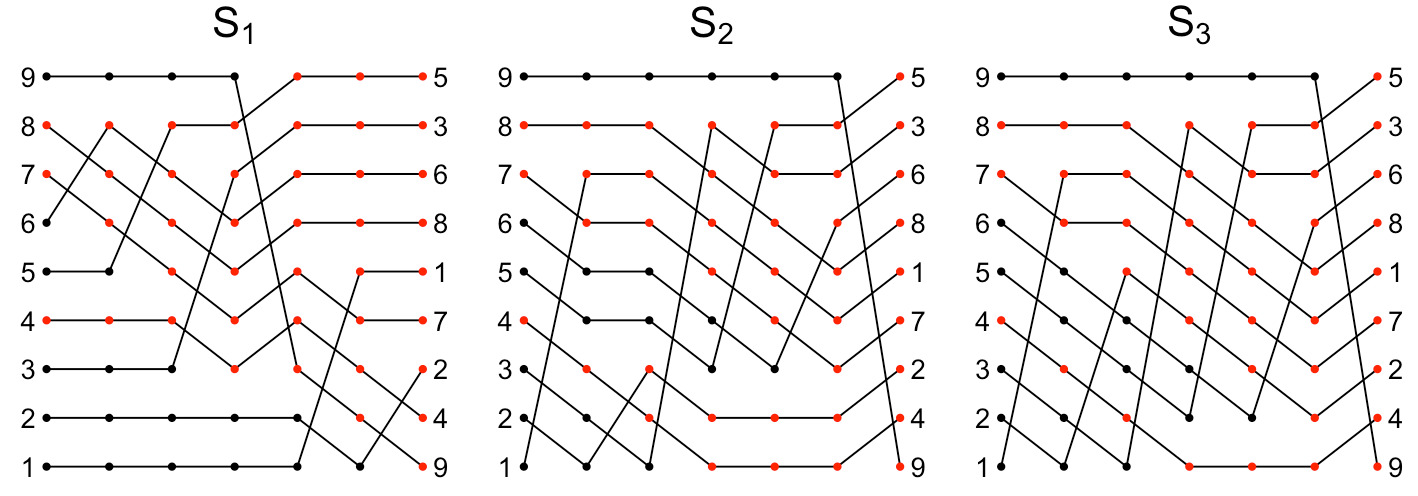
\includegraphics[width=0.80\textwidth]{crossings.png}
    \caption{Three sortings, $S_1$, $S_2$, and $S_3$, with $21$, $31$, and $35$ crossings, resp.}
    %. Each schedule, from left to right, . The greedy heuristic proposed to minimize~\ref{eq:schedule_opt_succ} was used to produce $S_1$, which has the minimal number of crossings, since $K_\tau(p,q) = 21$ in this example.
    \label{fig:crossings}
\end{figure}
%The greedy heuristic proposed to minimize equation~\ref{eq:schedule_opt_succ} was used to produce $S_1$, which has 21 edge crossings. 

\noindent  Each column represents the successive application of a move $m_{ij}$ in the schedule, 
and the edges track how each  symbol has been moved. 
Black/red vertices correspond to symbols in and outside of $\mathrm{LCS}$, respectively. 
All three schedules were generated from the same $\mathrm{LCS}(p,q) = (4\,7\,8)$ and all three schedules transform $p \mapsto q$ in $d = 6$ moves. 
In this example, $S_1$ matches the minimal number of crossings amongst all possible schedules,  since $K_\tau(p,q) = 21$. \\ \\
In general,  the $k$-layer crossing minimization problem for $k$ sets of permutations  is NP-hard for $k \geq 4$~\cite{biedl2009complexity}. As a result, we do not expect there to be a polynomial time algorithm for optimally achieving this proxy objective.  
% Since $\mathcal{D}$ is fixed, the complexity of a greedy strategy depends entirely on the complexity of minimizing $F(\hat{s}_i, \hat{s}_{i+1})$ at each greedy step.  
%For any sorting $S$ such that $s_{i}$ that increases the size of longest common subsequence between $s_{i-1} \circ \dots \circ s_1 \circ p$ and $q$. 
% and it satisfies a certain monotonicity property under LCS edit operations. 
%Specifically, given two permutations $p,q \in S_m$ with $\nu = \mathrm{LCS}(p,q)$ between them, the analysis in section~\ref{sec:move_schedules} shows we must move each symbol $x \in \mathcal{D}$ where $\mathcal{D} = p \smallsetminus \nu $ in a way that extends $\nu$ after each move. Each symbol $x \in \mathcal{D}$ induces a permutation $s_x$ such that $F(p, q) \geq F(s_x \circ p, q)$. That is, unlike the Kendall distance, the Spearman distance satisfies: 
%$$ F(p, q) \geq F(s_1 \circ p, q) \geq F( s_2 \circ s_1 \circ p, q) \geq F( s_d \circ \dots \circ s_1 \circ p, q)  = F(q,q) = 0 $$
%Since the complexity of the move operations discussed in section~\ref{sec:moves} depend on the size of the movement, it is advantageous to construct a schedule which minimizes this movement. 
%Since $\lvert \mathcal{D} \rvert$ is fixed, we would like to choose $x \in \mathcal{D}$ such that the corresponding permutation $s_x$ reduces the total displacement of every symbol $x \in \mathcal{D}$ relative to  $q$. 
%Substituting objective~\ref{eq:kendall_inequality} for $\mathrm{cost}(\cdot)$ in equation~\ref{eq:schedule_opt2} yields the following global optimization problem over $S_d$: 
%\begin{equation}\label{eq:schedule_opt_succ}
%S_{\sigma}^\ast = \argmin_{\sigma \in S_d} \frac{1}{2} \sum\limits_{i = 1}^{d - 1} F(\hat{s}_i, \hat{s}_{i+1})
%\end{equation}
%The minimizer of this optimization can be interpreted as a sorting which minimizes the net displacement amongst all possible $d$-sized sortings $p \mapsto q$, again in the $\ell_1$ sense. 
%A greedy strategy requires $O((d+(d-1)+(d-2)+\dots+1)m) \approx O(d^2 m)$ time to complete, since there are $O(d)$ symbols to choose from and minimizing $F(\hat{s}_i, \hat{s}_{i+1})$ at each step takes $O(md)$. 
%\\
%\\
%\noindent
%\textbf{Example:} We reconsider the greedy optimization example from section~\ref{sec:greedy}. 
%Table~\ref{table:greedy_costs} lists the \emph{successive} Kendall-$\tau$ and Spearman distances, respectively, between adjacent LCS edit (move) operations. Observe that, in this example, both greedy approaches lead to the schedule with minimal cost ($S_1$) (though this is not guaranteed in the general case).  
%\begin{table}[h]
%\caption{Move schedule costs (kendall and spearman)}
%\centering
%\begin{tabular}{ |P{0.4cm}|P{0.8cm}|P{0.8cm}|P{0.8cm}|P{0.8cm}|  }
% \hline
% \multicolumn{5}{|c|}{ Successive $K_\tau$ cost} \\
% \hline
% & 1st & 2nd & 3rd & Total\\
% \hline
% $S_1$ & 3 & 5 & 7 & 15 \\
% \hline 
% $S_2$ & 3 & 6 & 6 & 15 \\
%  \hline 
% $S_3$ & 4 & 4 & 7 & 15 \\
%  \hline 
% $S_4$ & 4 & 6 & 5 & 15 \\
%  \hline 
% $S_5$ & 5 & 6 & 6 & 17 \\
%  \hline 
% $S_6$ & 5 & 5 & 5 & 15 \\
% \hline
%\end{tabular}
%\quad 
%\begin{tabular}{ |P{0.4cm}|P{0.8cm}|P{0.8cm}|P{0.8cm}|P{0.8cm}|  }
% \hline
% \multicolumn{5}{|c|}{ Successive $F$ cost} \\
% \hline
% & 1st & 2nd & 3rd & Total\\
% \hline
% $S_1$ & 3 & 3 & 3 & 9 \\
% \hline 
% $S_2$ & 3 & 4 & 4 & 11 \\
%  \hline 
% $S_3$ & 4 & 4 & 3 & 11 \\
%  \hline 
% $S_4$ & 4 & 4 & 5 & 13 \\
%  \hline 
% $S_5$ & 5 & 4 & 4 & 13 \\
%  \hline 
% $S_6$ & 5 & 5 & 5 & 15 \\
% \hline
%\end{tabular}
%\label{table:greedy_costs}
%\end{table}  
%\\
%% TODO: elaborate on monotonicity, describe segment tree
However, the simplicity of both the Spearman distance and the types of permutations we consider here enables certain computational advantages. Suppose we begin with an array $\mathcal{A}$ of size $m$ which provides $O(1)$ access and modification, initialized with the (signed) \emph{displacement} of every element in $p$ to its corresponding position in $q$. Since the Spearman distance is simply the sum of the absolute value of these displacements, at any point during during the execution of Algorithm~\ref{alg:sorting} we may obtain $F(\bar{p}, q)$ simply by having access to the sum of every entry in $\mathcal{A}$. There are two degrees of freedom in   Algorithm~\ref{alg:sorting}: the first is in the choice of $\sigma \in \mathcal{D}$, and the second is in choosing $j$. If we fix a heuristic for the latter, then we have a set of possible valid moves $S_\mathcal{D}$ induced by each $\sigma \in \mathcal{D}$ to choose from. Observe that each permutation $s_\sigma \in S_\mathcal{D}$ changes the displacement of every symbol in at most three different ways: 
\[
\mathcal{A}(s_\sigma \circ p) = 
\begin{cases} 
	 \mathcal{A}(\sigma) \pm \lvert i - j \rvert & p^{-1}(\sigma) = i \\
	 \mathcal{A}(\sigma) \pm 1 & i < p^{-1}(\sigma) \leq j \\
	 \mathcal{A}(\sigma) & \text{ otherwise }
\end{cases}
\]
That is, if $s_\sigma$ represents a move permutation moving $\sigma$ from position $i$ to position $j$, then relative to the previous permutation $p$, the displacement of $\sigma$ in $s_\sigma \circ p$ changes by $\lvert i - j \rvert$ and the displacement of any symbol between $i$ and $j$ changes by $\pm 1$. 
All other symbol displacements are unchanged. Thus, if we replace $\mathcal{A}$ with a data structure  supporting $O(\log m)$ access time to aggregate information (i.e. the sum) and $O(\log m)$ modification time ability on $\lvert i - j \vert$ entries (simultaneously), we could greedily choose the next permutation $s$ to maximize:
\begin{equation}\label{eq:greedy_step}
	s_{\text{greedy}} = \argmin_{\text{ valid } s \in S_\mathcal{D}} F(s\circ p, q)
\end{equation}  
in $O(d\log m)$ time. 
The former problem reduces to the problem of efficiently calculating \emph{prefix sums}, which is easily solved. 
It is not immediately clear how to achieve the latter modification complexity in $O(\log m)$ time, since $\lvert i - j \rvert \leq m$ is potentially larger than $O(\log m)$.  
% Can actually only achieve O(d^2 log m) it seems 
It is known that one can apply constant-factor updates to multiple values in a prefix sum in $O(\log m)$ time by any prefix-sum data structure that also supports \emph{range updates}---e.g. an \emph{implicit treap}. 
Since single element modifications, removals, and insertions can all be achieved in $O(\log m)$ expected time with such a data structure, we conclude that a greedy solution to equation~\ref{eq:greedy_step} can be computed in $O(d^2 \log m)$ time. 
%Since single element prefix sum modifications can also be achieved $O(\log m)$ time with these data structures, the time to compute $F(\hat{s}_i, \hat{s}_{i+1})$ is bounded above by $O(\log m)$, 
%thus the greedy solution to equation~\ref{eq:schedule_opt_succ} can be computed in $O(d^2 \log m)$ time. 

%  e.g. a Fenwick tree, or a Segment Tree that supports lazy propagation~\cite{de1997computational}

%We give an example and a more detailed discussion for those interested in the appendix\ref{sec:appendix}. 
%This cumulative Spearman distance enables certain computational advantages. Suppose we begin with an array $\mathcal{D}$ of size $m$ which provides $O(1)$ access and modification, initialized to $0$, whose entries represent the summands of equation~\ref{eq:schedule_opt_succ}. 
%observe that each entry 
%
%%\begin{align}
%%	
%%\end{align}
%%$$ \argmin_{\sigma \in S_d} \frac{1}{2} \sum\limits_{i = 1}^{d - 1} F(\hat{s}_i, \hat{s}_{i+1}) = \argmin_{\sigma \in S_d} \frac{1}{2} \sum\limits_{i = 1}^{d - 1}  \sum\limits_{i \in [m]} \lvert \hat{s}(i) - \hat{s}_{i+1}(i) \rvert$$ 
%%
%% = 
%
%such that summing the entries in this array yields the Spearman distance in $O(m)$ time, which at initialization represents $F(p, p)$. Each symbol $x \in \mathcal{D}$ induces a  permutation $s_x$ such that $F(p, q) \geq F(s_x \circ p, q)$. Since there are $d = \lvert \mathcal{D} \rvert$ symbols to move and computing $F$ takes $O(m)$ time, a na\"ive greedy strategy requires $O((d+(d-1)+(d-2)+\dots+1)m) \approx O(d^2 m)$ time to complete. However, observe that each permutation $s_x$ changes the displacement of every symbol in a very predictable way: if $s_x$ represents a move permutation that moves $x$ from position $i$ to position $j$, then relative to the previous permutation $s_{i}$, the displacement of $x$ in $s_{i+1}$ changes by at most  $\lvert i - j \rvert$ and the displacement of any symbol between $i$ and $j$ changes by $\pm 1$. All other symbols are unaffected. Since the Spearman distance is simply the sum of these displacements, replacing $\mathcal{A}$ with a structure that supports both $O(\log m)$ access time to aggregate information (such as the sum) and $O(\log m)$ modification time ability to up to $\lvert i - j \vert$ entries. 
%The former problem reduces to the problem of efficiently calculating and updating \emph{prefix sums}, however since $\lvert i - j \rvert \leq m$ is potentially larger than $O(\log m)$, it's not immediately clear how to achieve the latter modification complexity in $O(\log m)$ time. Fortunately, since every elements displacement other than $x$ changes by $\pm 1$ per update, both queries can be efficiently done in $O(\log m)$ time using a Segment Tree that supports \emph{lazy propagation}~\cite{de1997computational}. 


%Suppose we precompute for each symbol $\sigma \in p$ its displacement relative to $q$, $| p(i) - q(i) |$, and store these displacements in an array providing $O(1)$ access and modification. 
%each LCS edit operation changes the distance by one of {-1, 0, +1}.  
% To obtain the first greedy step, this must done for all $d$ potential symbols to move, making the first step $O(dm)$. Upon applying an operation s_1 \circ p, every symbol that was moved must have its displacement updated. A naive solution would be to update the vector as-is, recomputing the new spearman distance for each candidate symbol to move. However, notice that the change in displacement for each symbol is limited to one of three options: {-1, 0, +1}. We may update this vector by utilizing a clever trick called \emph{lazy propagation}, a trick to a well known data structure called a segment tree. Updates take O(\log m) time, as do queries, reducing the complexity to $O(m + d log d)$ time. 


% TODO: Move computational results to subsection, add applications
% \subsection{Empirical results}\label{sec:results}
% \section{Applications and Discussion}\label{sec:applications}
\section{Empirical results}\label{sec:results}
\subsection*{Crocker stacks}
There are many challenges to depicting topological behavior in dynamic settings. One approach is to trace out the curves constituting a continuous family of persistence diagrams in $\mathbb{R}^3$---the vineyards approach---however this visualization can be cumbersome to work with as there are potentially many such vines tangled together, making topological critical events with low persistence difficult to detect. Moreover, the vineyards visualization does not admit a natural simplification utilizing the stability properties of persistence, as individual vines are not stable: if two vines move near each other and then pull apart without touching, then a pairing in their corresponding persistence diagrams may cross under a small perturbation, signaling the presence of an erroneous topological critical event~\cite{topaz2015topological, xian2020capturing}. 

\begin{figure}[t]
	\centering
	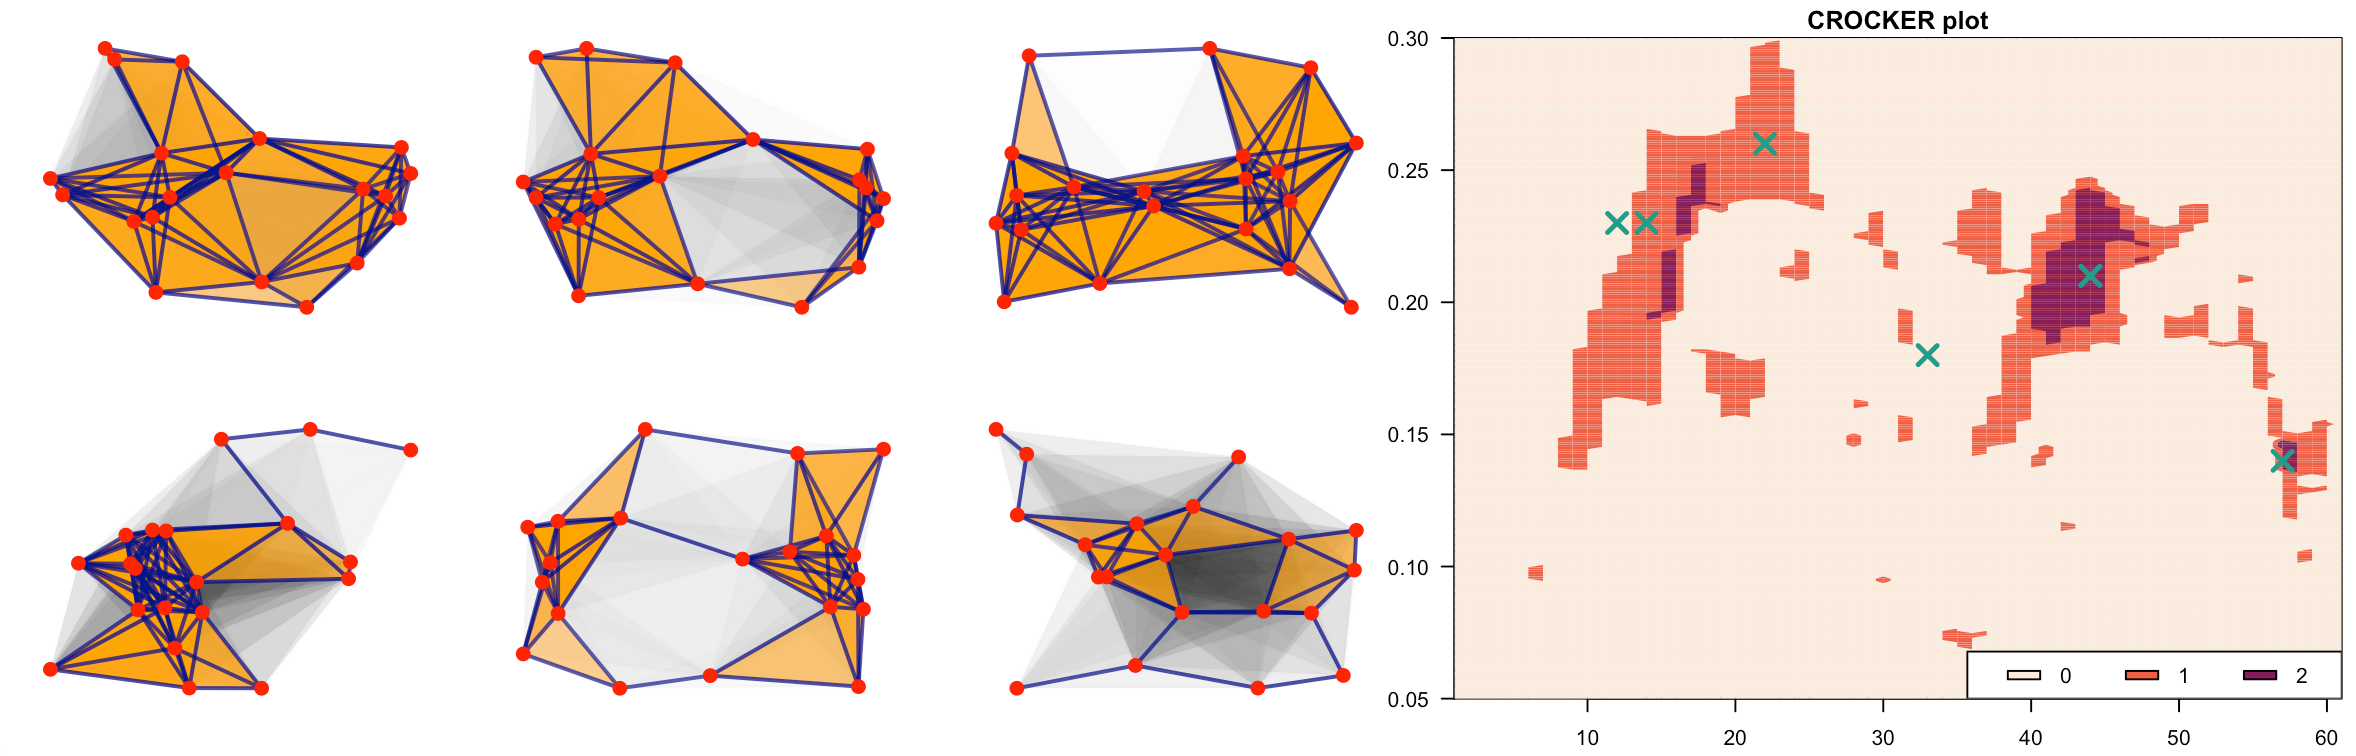
\includegraphics[width=0.95\textwidth]{crocker_combo_1.png}
	\caption{An example of a crocker plot (right) depicting the evolution of dimension $p = 1$ Betti curves over time. The green $\mathrm{X}$ marks correspond chronologically to the complexes (left), in row-major order. The large orange and purple areas depict $1$-cycles persisting in both space (the y-axis) and time (x-axis). }\label{fig:crocker1}
\end{figure}

Acknowledging this, Topaz et al.~\cite{topaz2015topological} proposed the use of a 2-dimensional summary visualization, called a \emph{crocker}\footnote{\emph{crocker} stands for ``Contour Realization Of Computed k-dimensional hole Evolution in the Rips complex.'' Although the acronym includes \emph{Rips complexes} in the name, in principle a crocker plot could just as easily be created using other types of triangulations (e.g. \v{C}ech filtrations).} plot. 
In brief, a crocker plot is a contour plot on a family of Betti curves. Formally, given a filtration $K = K_0 \subseteq K_1 \subseteq \dots \subseteq K_m$, a $p$-dimensional \emph{Betti curve} $\beta_p^{\bullet}$ is defined as the ordered sequence of $p$-th dimensional Betti numbers:
$$ \beta_p^\bullet = \{ \, \mathrm{rank}(H_p(K_0)), \, \mathrm{rank}(H_p(K_1)), \, \dots, \, \mathrm{rank}(H_p(K_m))\, \}$$
Given a time-varying filtration $K(\tau)$, a crocker plot can be interpreted as a contour plot on the 1-parameter family of Betti curves $\beta_p^\bullet(\tau)$. A example of a crocker plot generated from the simulation described below is given in Figure~\ref{fig:crocker1}. Since only the Betti numbers at each simplex in the filtration are needed to generate these Betti curves, the persistence diagram is not directly needed to generate a crocker plot; it is sufficient to use e.g. any of the specialized methods discussed in~\ref{sec:related_work}. This dependence only on the Betti numbers makes crocker plots easier to compute than standard persistence, however what one gains in efficiency one loses in stability; it is known that Betti curves are inherently unstable with respect to small fluctuations about the diagonal of the persistence diagram. 

Acknowledging this, Xian et al.~\cite{xian2020capturing} showed that crocker plots may be \emph{smoothed} to inherit the stability property of persistence diagrams and reduce noise in the visualization. That is, when applied to a time-varying persistence module $M = \{M_t\}_{t \in [0, T]}$ an $\alpha$-smoothed crocker plot for $\alpha \geq 0$ is the rank of the map $M_t(\epsilon - \alpha) \to M_t(\epsilon + \alpha)$ at time $t$ and scale $\epsilon$. For example, the standard crock plot is a $0$-smoothed crocker plot. Allowing all three parameters ($t, \epsilon, \alpha$) to vary continuously leads to 3D visualization called an $\alpha$\emph{-smoothed crocker stack}.
\begin{definition}[crocker stack]
	A crocker stack is a family of $\alpha$-smoothed crock plots which summarizes the topological information of a time-varying persistence module $M$ via the function $f_M : [0, T] \times [0, \infty) \times [0, \infty) \to \mathbb{N}$, where:
	$$ f_M(t,\epsilon, \alpha) = \mathrm{rank}(M_t(\epsilon - \alpha) \to M_t(\epsilon + \alpha)) $$
\end{definition}
\noindent A crocker stack is a sequence of $\alpha$-smoothed crocker plots that vary over $\alpha \geq 0$, satisfying $f_M(t,\epsilon,\alpha) \leq f_M(t,\epsilon, \alpha)$ for all $\alpha \geq \alpha'$. Note that, unlike crocker plots, applying this $\alpha$ smoothing efficiently \emph{requires} the persistence pairing. Indeed, it has been shown that crocker stacks and stacked persistence diagrams (i.e. vineyards) are equivalent to each other in the sense that either one contains the information needed to reconstruct the other~\cite{xian2020capturing}. Thus, computing crocker stacks reduces to computing the persistence of a (time-varying) family of filtrations.

%To describe this formally, let $K_\tau^\epsilon$ denote a simplicial filtration with simplices $\sigma \in K_\tau^\epsilon$ whose function value $f_\tau(\sigma) \leq \epsilon$. The $\alpha$

We test the efficiency of computing the necessary information to generate these crocker stacks using a spatiotemporal data set to illustrate the applicability of our method. Specifically, we ran a \emph{flocking} simulation similar to the simulation run in~\cite{topaz2015topological} with $m = 20$ vertices moving around on the unit square equipped with periodic boundary conditions (i.e. $S^1 \times S^1$). We simulated movement by equipping the vertices with a simple set of rules which control how the individual vertices position change over time. Such simulations are also called \emph{boid} simulations, and they have been extensively used as models to describe how the evolution of collective behavior over time can be described by simple sets of rules.
The simulation is initialized with every vertex positioned randomly in the space; the positions of vertices over time is updated according to a set of rules related to the vertices acceleration, distance to other vertices, etc. To get a sense of the time domain, we ran the simulation until a vertex made at least 5 rotations around the torus. 
\begin{figure}[ht]
	\centering
	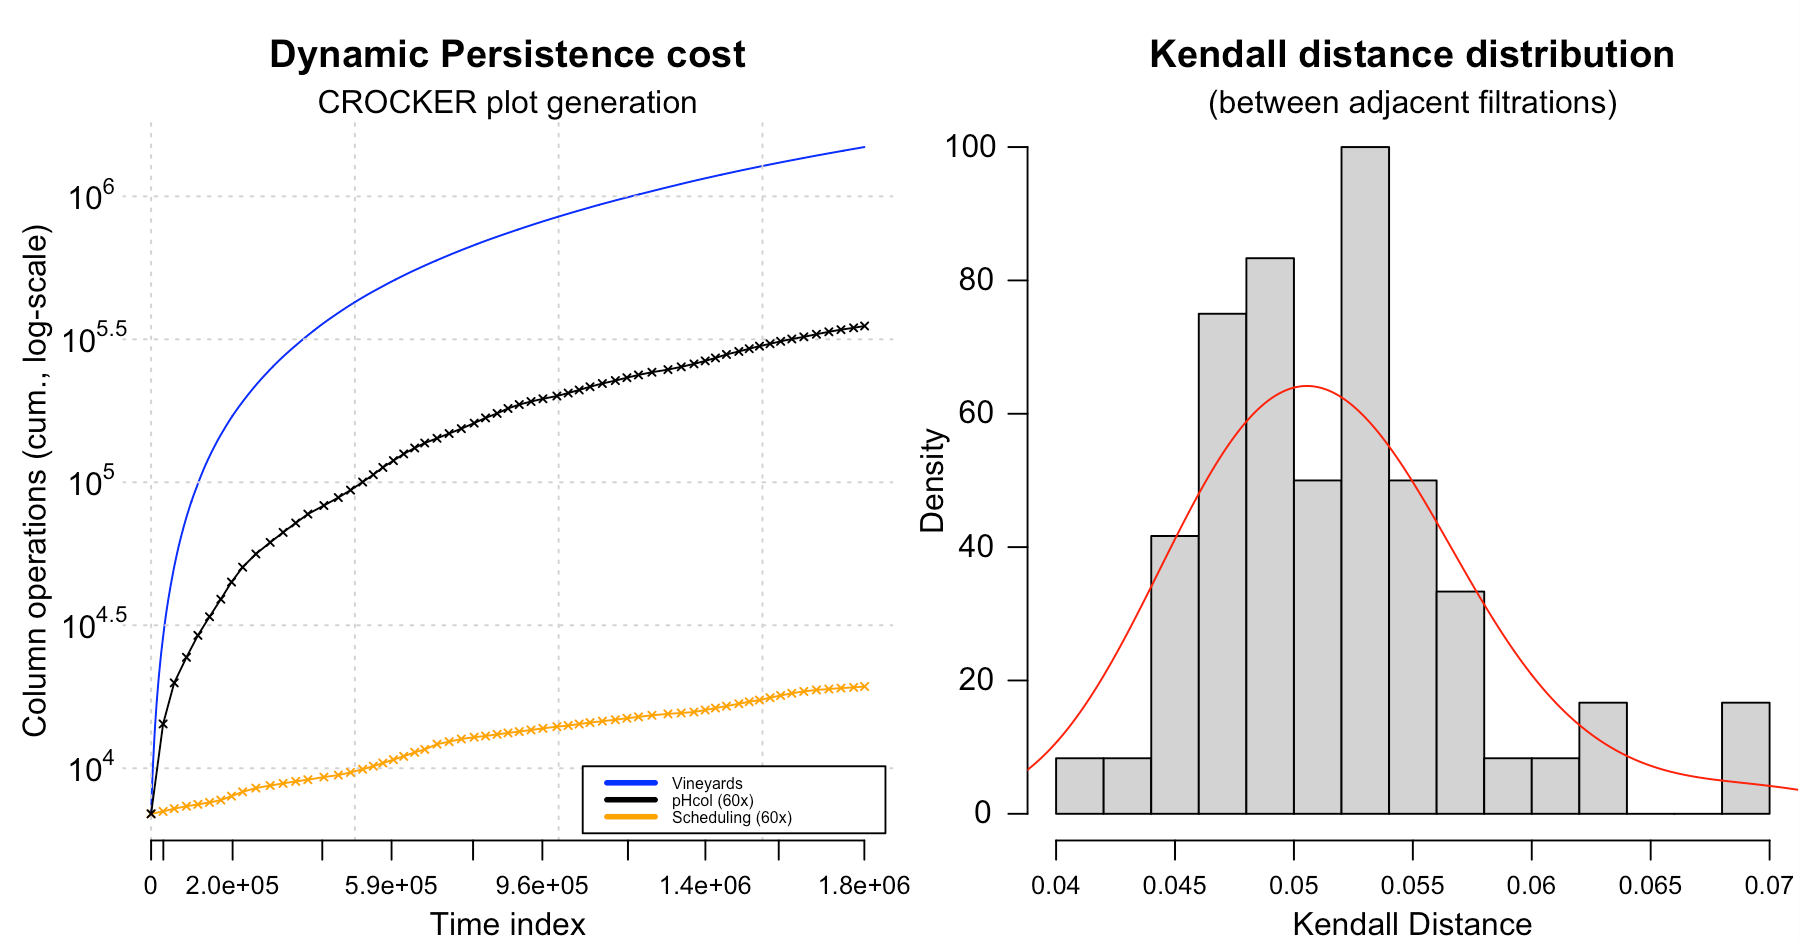
\includegraphics[width=\textwidth]{boid_sim_results.png}
	\caption{ The cumulative number of $O(m)$ column operations (left, log-scale) of the three approaches tested and the distribution of the normalized Kendall distance between adjacent filtration pairs. The histogram on the right depicts the coarseness of the discretization; most filtration pairs have $\approx 5\%$ of their $\approx O(m^2)$ simplex pairs inverted between adjacent time steps.}\label{fig:boid_sim_results}
\end{figure}

Given this time-evolving data set, we computed the persistence diagram of the Rips filtration up to $\epsilon = 0.30$ at 60 evenly spaced time points using three approaches: the standard algorithm \texttt{pHcol} applied naïvely at each of the 60 time steps, the vineyards algorithm applied to (linear) homotopy connecting filtrations adjacent in time, and our approach using moves.   
The cumulative number of $O(m)$ column operations executed by three different approaches. Note again that vineyards requires generating many decompositions by design (in this case, $\approx 1.8M$). The standard algorithm \texttt{pHcol} and our move strategy were computed at 60 evenly spaced time points of the simulations. As depicted in Figure~\ref{fig:boid_sim_results}, our move strategy is far more efficient then both vineyards and the naive \texttt{pHcol} strategies. 

\subsection*{Multidimensional persistence}
Given a procedure to filter a space in multiple dimensions simultaneously, a \emph{multifiltration}, the goal of multidimensional persistence is to identify persistent features by examining the entire multifiltration. 
Such a generalization has appeared naturally in many application contexts, showing potential as a tool for exploratory data analysis~\cite{lesnick2012multidimensional}. 
Indeed, one of the often noted drawbacks of persistence is its instability with respect to strong outliers. 
Although persistence diagrams are stable with respect to their input---in the Hausdorff sense---and thus are robust to Hausdorff noise, the presence of strong outliers can artificially modify the connectivity of the underlying filtration, obscuring the detection of what would otherwise be significant topological structures~\cite{buchet2015topological}. 
%Indeed, since inferring the homology of some underlying topological space around which data are distributed was one of the original purposes of persistence\footnote{One of the first uses of persistence was to infer the topology of attractors in dynamical systems from experimental data\cite{perea2018brief}.}, strong outliers pose a significant barrier to the widespread adoption of persistent homology. 
By filtering the data according to a notion of density, in tandem with distance predicates, multidimensional persistence can enable the practitioner to handle outliers directly.
%, without resorting to sophisticated data preprocessing techniques which may or may not preserve the underlying topology. 

Unfortunately, multidimensional persistent homology comes with its own set of computational and theoretical challenges. 
%not necessarily inherited by the 1-D case. 
There is not complete discrete invariant for multidimensional persistence---like the 1D persistence diagram---and the computations associated to other incomplete invariants exhibit high algorithmic complexity. A number of computational strategies have been proposed to counter this, such as homology preserving multifiltration simplification or parallelization schemes using shared-memory computation~\cite{fugacci2019chunk}. Rather than attempting to tackle multiple dimensions simultaneously, another approach is to focus on a fixed dimension, such as 2-D persistence. Utilizing the equivalence between the rank and fibered barcode invariants, Lesnick and Wright~\cite{lesnick2015interactive} developed an elegant way of visualizing the former via a reparameterization of the latter using standard point-line duality. This clever reparameterization effectively reduces the fibered barcode computation to a sequence of 1-D barcode computations at ``template points'' lying within the 2-cells of particular planar subdivision of the half-plane $[0, \infty) \times \mathbb{R}$. Indeed, since algorithm~\ref{alg:schedule} was designed for precisely such a computation, the algorithm proposed by~\cite{lesnick2015interactive} is prototypical of the class of methods that stand to benefit from move scheduling. 

The purpose of the following sections is to uncover the intrinsic bottlenecks impeding the computation of the fibered barcode invariant in practical settings. Towards this goal, we briefly summarize the theory established by several researchers~\cite{lesnick2015interactive, carlsson2010computing, landi2014rank}, focusing on their computational and algorithmic details. 
Our goal is to show that the highest complexity subcomputation of the fibered barcode invariant algorithm proposed by~\cite{lesnick2015interactive} is precisely the type of computation we focus on in this effort. 
In doing so, we substantiate our claims from section~\ref{sec:motivation} that our scheduling approach can improve the efficiency of a real-world application of multidimensional persistence by an order of magnitude by comparing Algorithm~\ref{alg:schedule} to several alternatives on a real-world data set and problem: the problem of identifying the underlying topological space of a data set extracting from high-contrast natural images. 
% In what follows, we briefly recount an incomplete but nonetheless very useful invariant of multi-dimensional persistence modules, the \emph{rank invariant}, as well as another invariant which in some sense determines the rank invariant, the \emph{fibered barcode}. It turns out that computing the latter invariant 

% --- For each section of the paper, consider writing a mini-introduction that says what its organization is, what is in each subpart, and how the parts relate to one another.

%To demonstrate how our scheduling approach can accelerate the multidimensional persistence computation, we establish the computational framework we will be considering. 
% These transforms end up being crucial in decomposing the definition of the fibered barcode (and thus, the rank invariant) into a discrete computation.
%We begin with a few definitions. An $n-D$ \emph{filtration} is a functor $\mathcal{F} : \mathbb{R}^n \to \textbf{Simp}$, the category of simplicial complexes, such that for all $a \leq b$, $\mathcal{F}(a,b) : F_a \to F_b$ is an inclusion. We will focus exclusively on the case where $n = 2$, where the object of study is a \emph{bifiltration}. Multifiltrations can be broadly categorized into two types: 1-critical and multi-critical filtrations. A \emph{1-critical filtration} $\mathcal{F}$ is a finite $n-D$ filtration each simplex $s \in K$ is associated with only one multi-grade (denoting its appearance in each of the filtered dimensions), otherwise $\mathcal{F}$ is said to \emph{multi-critical}. 
%An $n-D$ persistence module is a functor $M : \mathbb{R}^n \to \textbf{Vect}$, where $\textbf{Vect}$ denotes the category of $\mathbf{F}$-vector spaces and linear maps for some suitable field $\mathbb{F}$. A module $M$ is said to be \emph{pointwise finite dimensional} (p.f.d) if $\mathrm{dim}(M_a) < \infty$ for all $a \in \mathbb{R}^n$.
%For $i \geq 0$, let $H_i : \textbf{Simp} \to \textbf{Vect}$ denote the $i^{\text{th}}$ simplicial homology functor with coefficients in $\mathbb{F}$. 
%Using this notation, given a 1D filtration $\mathcal{F}$ of size $m$, each p.f.d 1D persistence module $M = H_i(\mathcal{F})$ for  may be associated with a multiset $\mathcal{B}(M)$ of intervals in $\mathbb{R}$ which record the isomorphism classes of indecomposable summands of $M$. The set $\mathcal{B}(M)$ is called the \emph{barcode}\footnote{Note that \emph{barcodes} and \emph{persistence diagrams} are interchangeable representations of the same multiset.} of $M$.
%\emph{The rank invariant} proposed by Carlsson et al~\cite{carlsson2009theory} is one such invariant that is complete when $n=1$ but is otherwise incomplete when $n \geq 2$. 
%% The rank invariant is computable in polynomial time~\cite{carlsson2010computing}, that has been the subject of much interest lately. 
%It is defined as follows: 
%\begin{definition}[Rank Invariant]
%	For $n \geq 1$, the \emph{rank invariant} of a $\mathbb{R}^n$-indexed persistence module $M$ over $\mathcal{H}^{n} \subseteq \mathbb{R}^n \times \mathbb{R}^n$ is the function:
%	\begin{equation*}
%		\begin{aligned}
%		& \mathrm{rank}(M)  \; : & \mathcal{H}^n & \to \mathbb{N}  \\
%		& & (a,b) & \mapsto \mathrm{rank} \, M(a,b) 
%		\end{aligned}
%	\end{equation*}
%	for $a \leq b \in \mathcal{H}^n$. When $n = 1$, the rank invariant is complete, thus $\mathrm{rank}(M)$ and the persistence barcodes $\mathcal{B}(M)$ determine each other.
%\end{definition}
%\noindent Thus, in one dimension, persistent homology provides a complete invariant that fully captures the lifetime of topological features in a given filtration: 1-D persistent homology modules decompose in an essentially unique way into indecomposable summands~\cite{zomorodian2005computing}. In contrast, the theory of multidimensional persistence shows that no complete discrete invariant exists---the structure of the target for the invariant depends on the structure of the underlying field, and although multiparameter persistence modules also decompose in a similar way as the 1-D case, the set of isomorphism classes is known to be extremely complicated~\cite{carlsson2009theory, lesnick2015interactive}. 
%Nonetheless, there are invariants related to multi-parameter persistence that can be quite useful in practice, even though they are incomplete. 
%\noindent For example, even though the rank invariant does not encode the isomorphism type of the underlying module $M$ when $n > 1$, it does captures important ``first-order'' information about the modules structure. 
 %The multigraded Betti numbers constitute a natural and important class of invariants often studied in algebraic geometry commutative algebra. There are many ways of defining these, with perhaps the simplest definition stemming from minimal resolutions: for a finitely generated $n$-parameter persistence module $M$ and $i \in \{0, 1, \dots, d \}$, the $i^{\text{th}}$ graded Betti number of $M$ at grade $z$, denoted as $\beta_i^M(z)$, is defined as the number of elements at grade $z$ in a basis of the $i^{\text{th}}$ module in a free resolution for $M$. 

\subsubsection*{The Fibered Barcode}
%In the context of persistence, and \emph{invariant} is a function from the collection of persistence modules to some set $S$ with the property that $f(M) = f(M')$ when $M \cong M'$. An invariant is said to be \emph{complete} if $M \cong M'$ whenever $f(M) = f(M')$. Thus, incomplete invariants are invariants which may have the same value on two non-isomorphic modules. 
Lesnick and Wright~\cite{lesnick2015interactive} associate three simple invariants to a 2-dimensional persistence module $M$: the \emph{dimension function}, the \emph{multigraded Betti numbers}, and the \emph{fibered barcode}. 
The dimension function is simply the the function which maps every point $a \in \mathbb{R}^2$ to $\mathrm{dim}(M_a)$. It is a simple and easy to visualize invariant, but is unstable and yields no information about the persistent features of $M$. 
The multigraded Betti numbers constitute a natural and important class of invariants often studied in algebraic geometry and commutative algebra, though both their theory and computation is beyond the scope of this effort---the interested reader is referred to~\cite{lesnick2015interactive, carlsson2009theory} for more details. For our purposes, the $i^{\text{th}}$-graded Betti number of $M$ is simply a function $\beta_i(M): \mathbb{R}^2 \to \mathbb{N}$ whose values indicate the the number of elements at  each degree in a basis of the $i^{\text{th}}$ module in a free resolution for $M$. 
The fibered barcode, denoted as $\mathcal{B}(M)$, is defined as follows: 
\begin{definition}[Fibered barcode]
	%\in \overline{\mathcal{L}}
	The fibered barcode $\mathcal{B}(M)$ of a 2D persistence module $M$ is the map which sends each line  $L \subset \mathbb{R}^2$ with non-negative slope to the barcode $\mathcal{B}_L(M)$: 
%	$$ L \mapsto \mathcal{B}_L(M) $$
$$ \mathcal{B}(M) = \{ \; B_L(M) : L \in \mathbb{R} \times \mathbb{R}^{+} \; \}$$
\end{definition} 
\noindent Thus, given a bipersistence module $M$, the fibered barcode of $M$ is the 2-parameter family of barcodes given by restricting $M$ to the of set affine lines with non-negative slope in $\mathbb{R}^2$. 

Although the fiber barcode is a very intuitive invariant, it is not clear how one might go about computing it efficiently. 
One could compute the 1-D persistence associated to some fixed linear combination of two given filter functions; each linear combination parameterizes a line $L \in \mathbb{R} \times \mathbb{R}^{+}$ which $M$ restricts too. 
However, this is an $O(m^3)$ time computation, which is prohibitive for exploratory data analysis purposes. 
Ideally, one would want to continuously vary $L \in \mathbb{R} \times \mathbb{R}^{+}$ interactively, inspecting the corresponding changes to the barcodes immediately. To enable this, ~\cite{lesnick2015interactive} introduced an elegant reparameterization that not only fully characterizes $\mathcal{B}(M)$, but also yields an efficient method for rendering $\mathcal{B}_L(M)$ in real time. In the next section, we briefly summarize this reparameterization. 

%The fibered barcode enjoys a number of stability properties readily expressed using interleaving distances~\cite{landi2014rank}. 
% More important to this work, the fibered barcode $\mathcal{B}(M)$ and the rank invariant $\mathrm{rank}(M)$ determine each other~\cite{lesnick2015interactive}. 

\subsubsection*{Reparameterization using point-line duality}\label{sec:fibered_barcode_reparam}
Let $\overline{\mathcal{L}}$ denote the collection of all lines in $\mathbb{R}^2$ with non-negative slope, $\mathcal{L} \subset \overline{\mathcal{L}}$ the collection of all lines in $\mathbb{R}^2$ with non-negative, finite slope, and $\mathcal{L}^\circ$ the collection of all affine lines in $\mathbb{R}^2$ with positive, finite slope. There is a standard point-line duality that gives a parameterization of $\mathcal{L}$ with the half-plane $[0, \infty) \times \mathbb{R}$ that is convenient to work with here. Define the \emph{line} and \emph{point} dual transforms $\mathcal{D}_{\ell}$ and $\mathcal{D}_p$, respectively, as follows: 
\begin{equation}
	\begin{aligned}
\mathcal{D}_{\ell}: \mathcal{L} \rightarrow[0, \infty) \times \mathbb{R} & \quad \hfill \quad & \mathcal{D}_{p}:[0, \infty) \times \mathbb{R} \rightarrow \mathcal{L} \\
y=a x+b \mapsto(a,-b) &\quad \hfill \quad & (c, d) \mapsto y=c x-d
\end{aligned}
\end{equation}
% Use \multicolumn{1}{|r|}{text} to align
The transforms $\mathcal{D}_{\ell}$ and $\mathcal{D}_p$ are \emph{dual} to each other in the sense that for any point $a \in [0, \infty) \times \mathbb{R}$ and any line $L \in \mathcal{L}$, $a \in L$ if and only if $D_\ell(L) \in D_{p}(a)$. Now, for some fixed line $L$, define  the \emph{push map} $\mathrm{push}_L(a):  \mathbb{R}^2 \to L \cup \infty$ as: 
\begin{equation}
	\mathrm{push}_L(a) \mapsto \mathrm{min}\{ v \in L \mid a \leq v \}
\end{equation}
%\begin{equation*}
%	\begin{aligned}
%	& \mathrm{push}_L : & \mathbb{R}^2 & \to L \cup \infty \\
%	& & a \in \mathbb{R}^2 & \mapsto \mathrm{min}\{ v \in L \mid a \leq v \}
%	\end{aligned}
%\end{equation*}
The push map satisfies a number of useful properties. Namely: 
\begin{enumerate}
	\item For $r < s \in \mathbb{R}^2$, $\mathrm{push}_L(r) \leq \mathrm{push}_L(s)$
	\item For each $a \in \mathbb{R}^2$, $\mathrm{push}_L(a)$ is continuous on $\mathcal{L}^\circ$
	\item For $L \in \mathcal{L}^\circ$ and $S \subset \mathbb{R}^2$, $\mathrm{push}_L$ induces a totally ordered partition $S_L$ on $S$ 
\end{enumerate}
Property (1) asserts that for any $L \in \overline{\mathcal{L}}$, the standard partial order on $\mathbb{R}^2$ restricts to a total order on $L$. Properties (2) and (3) qualify the following definition:
\begin{definition}[Critical Lines]
	For some fixed $S \subset \mathbb{R}^2$, a line $L \in L^\circ$ is defined to be \emph{regular} if there is an open ball $B \in L^\circ$ containing $L$ such that $S_L = S_{L'}$ for all $L' \in B$. Otherwise, the line $L$ is defined as \emph{critical}. 
\end{definition}
\noindent The set of critical lines $\mathrm{crit}(M)$ with respect to some fixed set $S \subset \mathbb{R}^2$ fully characterizes a certain planar subdivision of the half plane $[0, \infty) \times \mathbb{R}$. 
This planar subdivision, denoted by $\mathcal{A}(M)$, is thus entirely determined by $S$ under point line duality.
%It has been shown~\cite{lesnick2015interactive} that the 1-skeleton $\mathcal{A}^1(M)$ of the line arrangement $\mathcal{A}(M)$ can be characterized b
%Explicitly, define $\mathcal{A}^1(M)$ to the 1-skeleton of the line arrangement defined by: 
% \{ \mathcal{D}_p(\alpha) \text{ for } \alpha = \mathrm{LUB}(u,v), u,v \in S \} 
%\begin{equation}\label{eq:arrangement_crit}
%	\mathcal{A}^1(M) = \{ \mathcal{D}_{\ell}(\mathrm{crit}(M)) \cup (\{0\} \times \mathbb{R}) \}
%\end{equation}
%Expanding the 1-skeleton to a 2-D cell complex $\mathcal{A}(M)$ fully partitions the upper half plane.  
A corollary from~\cite{lesnick2015interactive} shows that if the duals of two lines $L, L' \in \mathcal{L}$ are contained in the same $2$-cell in $\mathcal{A}(M)$, then $S_L = S_{L'}$, i.e. the partitions induced by $\mathrm{push}_L$ are equivalent. Indeed, the total order on $S_L$ is simply the pullback of the total order on $L$ with respect to the push map.
Since $\mathcal{A}(M)$ partitions the entire half-plane, the dual to every line $L \in \mathcal{L}$ is contained within $\mathcal{A}(M)$---the desired reparameterization. 

Let $S = \mathrm{supp}\,\beta_0(M) \, \cup \, \mathrm{supp}\,\beta_1(M)$, where the functions $\beta_0(M), \beta_1(M)$ are $0^{\text{th}}$ and $1^{\text{st}}$ bigraded Betti numbers of $M$, respectively. 
The main mathematical result from~\cite{lesnick2015interactive} is a characterization of the barcodes $\mathcal{B}_L(M)$, for any $L \in \mathcal{L}$, in terms of a set of \emph{barcode templates} $\mathcal{T}$ computed at every 2-cell in $\mathcal{A}(M)$.
 More formally, for any line $L \in \overline{\mathcal{L}}$ and $e$ any 2-cell in $\mathcal{A}(M)$ whose closure contains the dual of $L$ under point-line duality, the 1-parameter restriction of the persistence module $M$ induced by $L$ is given by: 
 \begin{equation}
 \mathcal{B}_L(M) = \{ [\,\mathrm{push}_L(a), \, \mathrm{push}_L(b)\,) \mid (a,b) \in \mathcal{T}^e, \mathrm{push}_L(a) < \mathrm{push}_L(b)  \} 
\end{equation}
Minor additional conditions are needed for handling completely horizontal and vertical lines. 
The importance of this theorem lies in the fact that the fibered barcodes are completely defined from the precomputed barcode templates $\mathcal{T}$---once every barcode template $\mathcal{T}^e$ has been computed and augmented onto $\mathcal{A}(M)$, $\mathcal{B}(M)$ is completely characterized, and the barcodes $\mathcal{B}_L(M)$ associated to a 1-D filtration induced by \emph{any} choice of $L$ can be efficiently computed via a point-location query on $\mathcal{A}(M)$ and a $O(\lvert \mathcal{B}_L(M) \rvert)$ application of the push map.

%For some fixed set $S \subset \mathbb{R}^2$ and any pair $u, v \in S$ of points which are incomparable with respect to the partial order on $\mathbb{R}^2$
% The definition of \emph{critical} lines provides an analogue to the 
 
%This is the main mathematical result from~\cite{lesnick2015interactive},

% Indeed, it was shown in~\cite{lesnick2015interactive} that the fibered barcodes $$ of $M$ (i.e. the collection of barcodes of 1D affine slices of $M$) and the rank invariant determine each other.     
\subsubsection*{Computing the fibered barcode}
%Lesnick and Wright introduced the Rank Invariant Visualization and Exploration Tool (RIVET)~\cite{lesnick2015interactive}, which is both a tool and a collection of computational and mathematical theory which enables exploratory analysis of 2D persistence modules built from arbitrary bifiltrations. From a computational perspective, the core novelty of the RIVET approach is its ability to compute the fibered barcodes efficiently from precomputed information. 
Given bipersistence module $M$, the three dominant computations needed to compute the fibered barcode using the reparameteratization discussed above are the following: 
\begin{enumerate}
	\item Computing the bigraded Betti numbers $\beta(M)$ of $M$
	\item Constructing a line arrangement $\mathcal{A}(M)$ induced by critical lines from (1) 
	\item Augmenting $\mathcal{A}(M)$ with a \emph{barcode template} $\mathcal{T}^e$ at every 2-cell $e \in \mathcal{A}(M)$
	%, yielding the \emph{augmented arrangement} $\mathcal{A}^{\sbullet}(M)$ 
\end{enumerate}
Computing (1) takes approximately $\approx O(m^3)$ using a matrix algorithm similar to Algorithm~\ref{alg:reduce}~\cite{lesnick2019computing}. Constructing and storing the line arrangement $\mathcal{A}(M)$ with $n$ lines and $k$ vertices is related to the \emph{line segment intersection problem}, which known algorithms in computational geometry can solve in (optimal) output-sensitive $O((n+k) \log n)$ time (see~\cite{boissonnat2000robust} for an overview). In terms of memory complexity, the number of 2-cells in $\mathcal{A}(M)$ is upper bounded by $O(\kappa^2)$, where $\kappa$ is a coarseness parameter associated with the computation of $\beta(M)$. 
By combining this bound with a bound on the number of transpositions needed to traverse a particular sequence of 2-cells in $\mathcal{A}(M)$, the analysis from~\cite{lesnick2015interactive} shows that the computation of the barcodes templates $\mathcal{T}$ from step (3) using vineyard updates requires on the order of $O(m^3 \kappa + m \kappa^2 \log \kappa)$ elementary operations and $O(m \kappa^2)$ storage. 

Of the three steps above, the barcode template computation is both the highest complexity and most demanding computation in practice. The number of 2-cells in $\mathcal{A}(M)$ is on the order $O(\kappa^2)$, and $\kappa$ itself is on the order of $O(m^2)$ in the worst case. 
This suggests the computation of the barcode templates is on the order $O(m^5)$, which is effectively intractable for even moderately-sized filtrations. In practice, the external stability result from~\cite{landi2014rank} justifies the use of a simple procedure which approximates the module $M$ with a smaller module $M'$ using a grid-like coarsening procedure. This coarsening procedure allows the practitioner to restrict the size of $\kappa$ to a relatively small constant, which in-turn dramatically reduces the size of $\mathcal{A}(M)$. 

There are several approaches one can use to compute $\mathcal{T}$, the simplest being to run Algorithm~\ref{alg:reduce} independently on the 1-D filtration induced by the duals of some set of points (e.g. the barycenters) lying in the interior of the 2-cells of $\mathcal{A}(M)$.  
The approach taken by~\cite{lesnick2015interactive} is to use the $R = DV$ decomposition computed at some adjacent 2-cell $e \in \mathcal{A}(M)$ to speed up the computation of an adjacent cell $e' \in \mathcal{A}(M)$. More explicitly, define the \emph{dual graph} of $\mathcal{A}(M)$ to be the undirected graph $G$ which has a vertex for every 2-cell $e \in \mathcal{A}(M)$ and an edge for each adjacent pair of cells $e, e' \in \mathcal{A}(M)$.
Each vertex in $G$ is associated with a barcode template $\mathcal{T}^e$, and the computation of $\mathcal{T}$ now reduces to computing a path $\Gamma$ on $G$ which visits each vertex at least once. To minimize the computation time, assume the $n$ edges of $G$ are endowed with non-negative weights $W = w_1, w_2, \dots, w_n$ whose values $w_i \in \mathbb{R}_{+}$ represent some notion of distance. The optimal path $\Gamma^\ast$ is the one of minimal length with respect to $W$ which visits every vertex of $G$ at least once. There is a known $\frac{3}{2}$-approximation that can be computed efficiently which reduces the problem to the traveling salesman problem on a metric graph~\cite{christofides1976worst}.
\\
\\
\textbf{Noisy circle example} We include a small example to illustrate many of the concepts and definitions discussed so far. 
Consider a small set of points distributed noisily around $S^1$ that contains a few strong outliers, shown on the left side of Figure~\ref{fig:bifiltration_ex2}. Filtering this data set with respect to the Rips parameter and the complement of a kernel density estimate yields a bifiltration whose dimension function and bigraded Betti numbers are shown in the middle figure. The gray areas indicate the region where the dimension function is constant; the lighter gray area where $\mathrm{dim}_1(M) = 1$, indicating where a persistent loop was detected.
On the right side, the space dual to the space in the middle is shown. The black lines represent the lines of $\mathcal{A}(M)$, the blue dashed-lines the edges of the dual graph $\mathcal{G}$, and the orange points the barycenters of the 2-cells in $\mathcal{A}(M)$, depicting where the barcodes templates $\mathcal{T}^e$ are parameterized. 
\begin{figure}[t]
	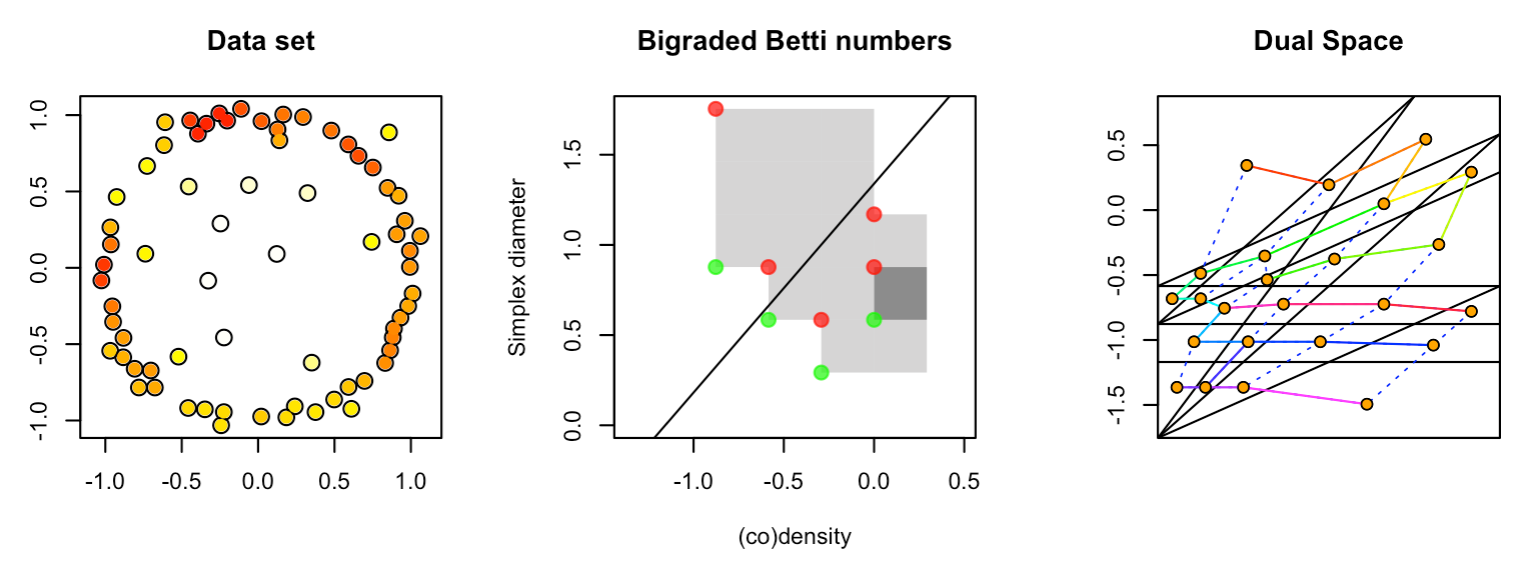
\includegraphics[width=0.98\textwidth]{bifiltration_ex2}
	\caption{Bipersistence example on an $8 \times 8$ coarsened grid. On left, the input data, colored by density. In the middle, the bigraded Betti numbers $\beta_0(M)$ and $\beta_1(M)$ (green and red, respectively), the Hilbert function (gray), and a line $L$ emphasizing the persistence of features with high density. On the right, the line arrangement $\mathcal{A}(M)$ lying in the dual space $D_p(\alpha)$ derived from the $\beta(M)$. }
	\label{fig:bifiltration_ex2}
\end{figure}
The shortest path $\Gamma^\ast$ spanning the vertices of $G$ is shown by the solid rainbow colored lines, with the traversal beginning in the top-left cell (at the red edge) and ending at the bottom-right cell (the indigo edge). Traversing $\Gamma^\ast$ can be done via a simple depth-first search, though note that a $R=DV$ decomposition needs to be stored at each degree-3 or higher vertex in $\Gamma^\ast$ to avoid redundant computations as the traversal recurses. 
\\

%To an along an Eulerian path spanning the dual graph $G$ of the arrangement $\mathcal{A}(M)$. The
%As input, one has a set of points $A \subset \mathbb{R}^2$, whose duals induce filtrations ww
%Since each template point corresponds to a dual 
%TODO: (Discuss path along dual graph of $\mathcal{A}(M)$)
% It is worth briefly discussing just how difficult computationally step (3) is. For a bifiltration with $m$ simplices, \emph{without any coarsening}, $\kappa$ is on the order of $O(m^2)$ in the worst case. Thus, the uncoarsened complexity of the template computation barcode is $\approx O(m^5)$, where again $m$ is the number of simplices in the bifiltration. A more common practice in data science is to report the complexity of algorithm in terms of the number of data points. Given some input point cloud data (PCD) with $n$ points, the standard rips filtration up to dimension 2 can have upwards of $O(n^3)$ 2-simplices. Thus, given a 2-dimensional bifiltration $\mathcal{F}$ with $m = n^3$ simplices derived from a rips filtration on PCD with $n$ data points, the complexity of computing all barcode templates for every $2$-cell in $\mathcal{A}(M)$ for $M = H_1(\mathcal{F})$ is on the order of $O((n^3)^5) \approx O(n^{15})$. This is clearly computationally intractable for even relatively small data sets. 

%There are a few ways of tackling this computational barrier. Recent work has focused on using alternative filtration whose size is much smaller than that of the rips (or cech) filtration, but whose homology is approximately the same, for example by using a sparsified rips filtration~\cite{} or the chunk-based approach to multi-parameter persistence~\cite{fugacci2019chunk}. It was shown in~\cite{} that one can alternatively opt to approximate a bipersistence module $M$ by a \emph{coarsened} module $M'$ in a way that bounds the the interleaving distance $d_I(M, M')$ between the two modules. The external stability result of Landi~\cite{} implies that if the two modules $M$ and $M'$ are close in their interleaving distance, then the fibered barcodes $\mathcal{B}(M)$ and $\mathcal{B}(M)$ will be close as well. In practice, this coarsening procedure is essential to enabling the practical computation of the fibered barcodes. 



% However, if a give bipersistence module $M$ is coarsened at all, the 
%  Specifically, assembling the barcode takes just $O(\log \kappa + \lvert \mathcal{B}_L(M) \rvert ) \approx O(\lvert \mathcal{B}_L(M) \rvert )$ time when $\kappa$, a coarsening parameter discussed below, is treated as a constant.  
 
 \subsubsection*{Natural images dataset} 
 In the previous section, we outlined the computational theory of multidimensional persistence, including its relevance to our proposed move scheduling approach. In this section, we demonstrate the efficiency of our method on practical use case of multidimensional persistence: detecting the presence of a low-dimensional topological space which well-approximates the distribution of texture patches extracted from real-world image data. 
 
 \begin{figure}[t]
	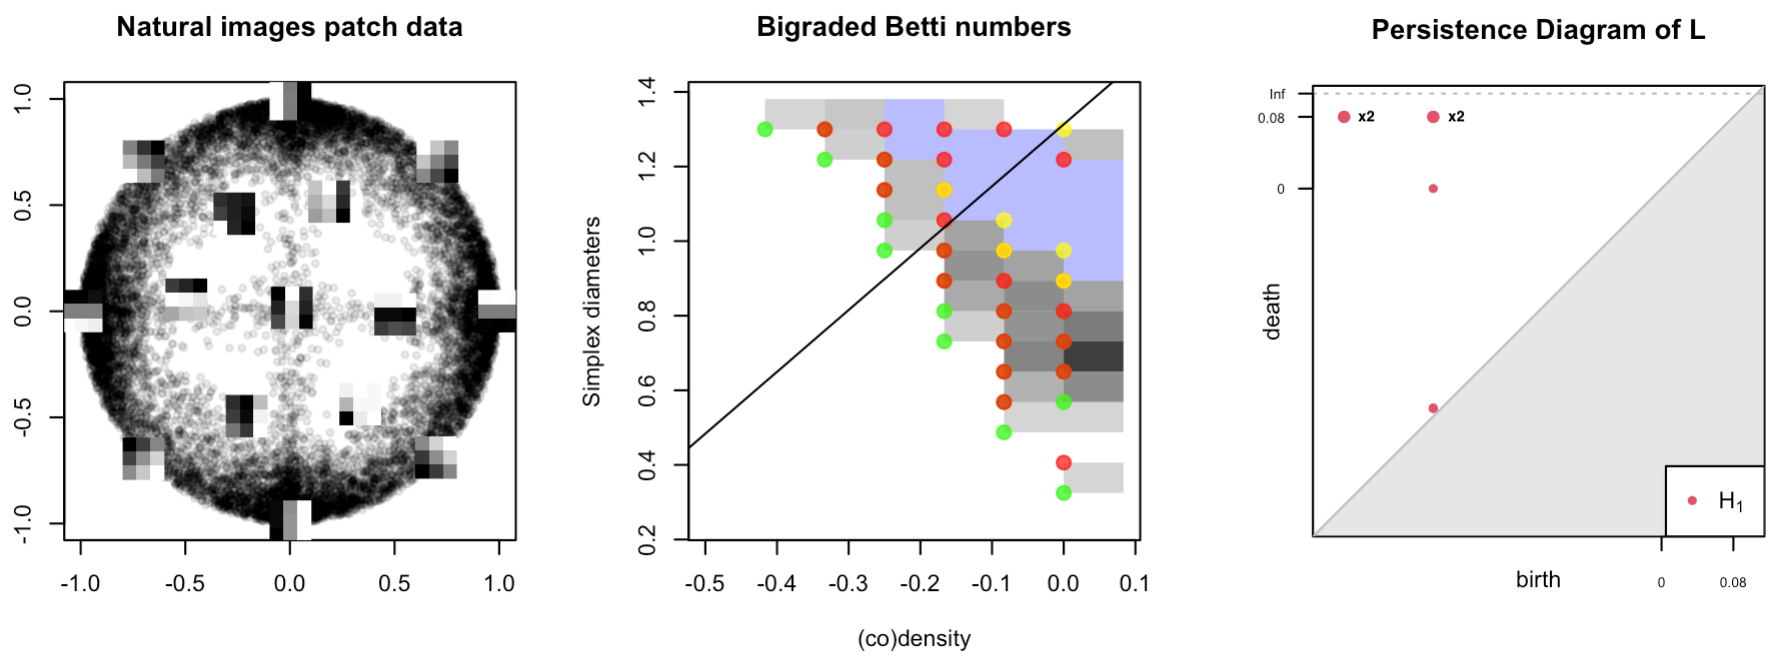
\includegraphics[width=0.98\textwidth]{natural_images}
	\caption{Bipersistence example of natural images data set on an $12 \times 16$ coarsened grid. On the left, a projection the full data set is shown, along with the 15 landmark patches. In the middle, the bigraded Betti numbers, the Hilbert function, and a chosen line $L$ are shown for the coarsened grid. As before, the $0/1/2$ dimension bigraded Betti numbers are shown in green/red/yellow, respectively. The blue regions highlights where $\mathrm{dim}(M) = 5$. On the right, the persistence diagram of $M$ restricted to $L$, with larger points indicating a multiplicity of 2. Observe five persistent features are revealed in both the middle and right plots, matching $\beta_1$ of the three-circle model. }
	\label{fig:patch_data_dgm}
\end{figure}

A common hypothesis is that high dimensional data tend to lie in the vicinity of an embedded, low dimensional manifold or topological space. An exemplary demonstration of this is given in~\cite{lee2003nonlinear}, who explored the space of $3 \times 3$ high-contrast patches extracted from Hans van Hateren's still image collection~\cite{hateren_schaaf_1998}, which consists of approximately 4,000 monochrome images\footnote{See \url{http://bethgelab.org/datasets/vanhateren/} for details on the image collection.} depicting various areas outside around Groningen (Holland). Motivated by applications to sparse coding applications, Lee et al.~\cite{lee2003nonlinear} was interested in how these natural image patches were distributed, in pixel-space, with respect to predicted spaces and manifolds. For example, one of the motivating questions of their research was whether there were any clear qualitative differences the distributions of patches extracted from from images of different modalities, e.g. optical versus range images. A major result from their work is that the majority of high-contrast image patches are concentrated around a 2-dimensional submanifold embedded in $S^7$.
Supplemental experiments conducted by Carllsson et al.~\cite{carlsson2008local} using persistent homology confirmed that the distribution of high-contrast $3 \times 3$ patches is indeed well-approximated by a Klein bottle---around 60\% of the high-contrast patches from the still image data set are concentrated within a small neighborhood around a model of a Klein bottle which accounts for $\approx$ 21\% of the volume $S^7$, compared to the $\approx$ 84\% of volume of $S^7$ accounted for by the entire data set. Along a similar vein, in the context of sparse coding, Perea et al.~\cite{perea2014klein} introduced a dictionary learning framework for estimating and representing the distribution of patches from texture images. 

If one was not aware of the analysis done by~\cite{lee2003nonlinear, hateren_schaaf_1998, carlsson2008local, perea2014klein}, it is not immediately clear a priori that the Klein bottle model is indeed a good candidate for capturing non-linearity of image patches. Nonetheless, as we have mentioned, among the first uses of persistent homology was the so-called ``homology inference problem''~\cite{perea2018brief}; given a suitable treatment of strong outliers using by e.g. filtering both on the geometry and the density of the image patches, the homology of the Klein bottle should become apparent through a persistence computation.
 
Consider the (coarsened) fibered barcode computed from a standard Rips / codensity bifiltration on a representative sample of the image data from~\cite{hateren_schaaf_1998} (details to follow), shown in Figure~\ref{fig:patch_data_dgm}. 
Upon inspection of the bigraded Betti number and the dimension function, one finds that a large area of dimension function is constant (highlighted as the blue portion in the middle of Figure~\ref{fig:patch_data_dgm}), wherein the first Betti number is 5. There are many spaces whose  meets this criterion, though upon further inspection, one candidate space that seems particularly plausible is the three-circle model $C_3$. The $C_3$ model consists of three circles, two of which (say, $S_v$ and $S_h$) intersect the third (say, $S_\mathrm{lin}$) in exactly two points, but themselves do not intersect. Upon performing an analysis on the density of the patches analogous to the one done by~\cite{lee2003nonlinear}, one finds that the mean-centered and contrast normalized $3 \times 3$ patches like on a 7-dimensional ellipsoid $\tilde{S}^7 \subset \mathbb{R}^9$. Contrast is typically measured using a discrete version of the Dirichlet semi-norm, or the ``$D$-norm'' $\lVert \cdot \rVert_D$ for short, which is a unique scale-invariant norm on images:
$$ \lVert x \rVert_D = \sqrt{\sum_{i \sim j}(x_i - x_j)^2} = \sqrt{x^T D x}$$
where $D$ is a fixed matrix which upon application to an image $x \in \mathbb{R}^9$ yields a value proportional to the sum of the differences between the 4-connected neighbors (described by the relation $i \sim j$). It is advantageous to ``whiten'' the data via a change of coordinates to Euclidean sphere. 
This can be achieved by expressing the patch data as an expansion of a certain convenient basis of 8 non-constant eigenvectors, often called the Discrete Cosine Transform (DCT) basis~\cite{lee2003nonlinear}, which are given below: 
%\vspace{-0.2em}
\begin{center}
	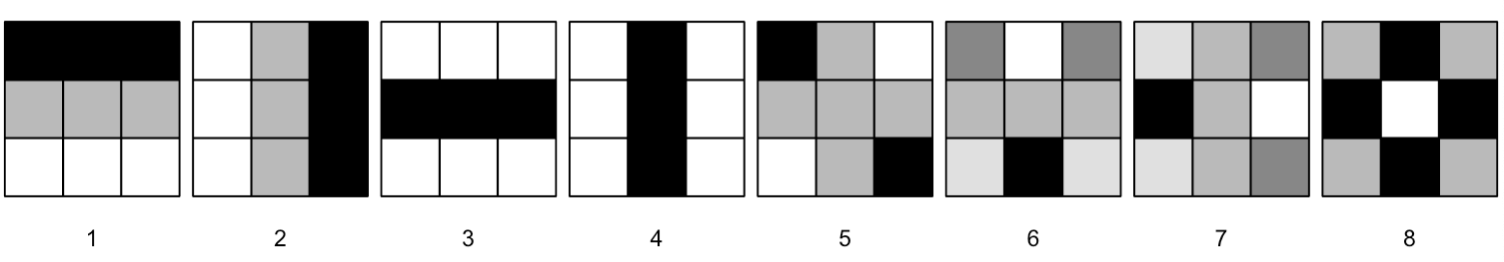
\includegraphics[width=0.80\textwidth]{dct_basis} 
\end{center}
%\begin{figure}[h]
%	\captionsetup{labelformat=empty}
%	\centering
%	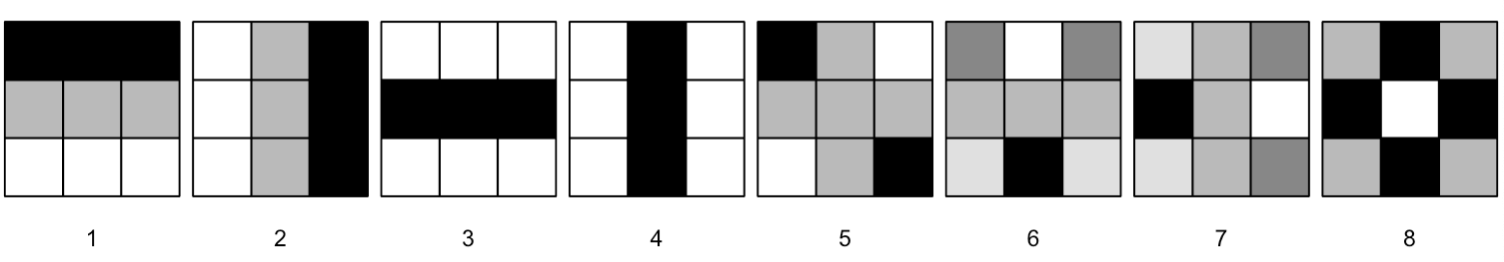
\includegraphics[width=0.90\textwidth]{dct_basis}
%	\caption{}
%\end{figure}
%\vspace{-1.5em}
\noindent Projecting the image data onto the first two basis vectors of leads to the projection shown in the top left of Figure~\ref{fig:patch_data_dgm}. 15 landmark points are also shown. Observe the data are distributed well around three ``circles''---the outside circle capturing the rotation gradient of the image patches ($S_{\mathrm{lin}}$), and the other two circles capturing the vertical and horizontal gradients ($S_v$ and $S_h$, respectively). Since the three circle model is the 1-skeleton of the Klein bottle~\cite{carlsson2008local}, one may conclude that the Klein bottle might be a reasonable candidate upon which the image data are distributed. This can be further verified empirically by e.g. using the iterative, meanshift-like procedure described in~\cite{carlsson2008local} to fit a parameterization of the model in question to the data. 

Using the same high-contrast patch data set studied in~\cite{lee2003nonlinear}, we evaluate the performance of various methods at computing the fibered barcode invariant using the parameterization from~\ref{sec:fibered_barcode_reparam}. 
Due to the aformentioned high complexity of the fibered barcode computation, we begin by working with a subset of the image patch data $\mathcal{X}$. Specifically, we combine the use furthest-point sampling and proportionate allocation (stratified) sampling to sample landmarks $X \subset \mathcal{X}$ distributed within $n = 25$ strata. Each strata consists of the $(1/n)$-thick level set given by $\rho_{15}$, the density estimator. The use of furthest-point sampling gives us certain coverage guarantees that the geometry is approximately preserved within each level set, whereas the stratification ensures the original density of is approximated preserved as well. From this data set, we construct a Rips-(co)density bifiltration using $\rho_{15}$ equipped with the geodesic metric computed over the same $k = 15$ knn graph on $X$. 
Finally, we record the number of column reductions needed to compute the fibered barcode at a variety of levels of coarsening using $\mathtt{pHcol}$, vineyards, and our moves approach. The results are summarized in Table~\ref{tab:barcode_templates}. We also record the number of 2-cells encountered along the path $\Gamma$ permutations that were applied throughout the computation of the barcode templates for both vineyards and moves, denoted in the table as $d_K$ and $d_{\mathrm{LCS}}$, respectively. 
%Specifically, we begin by extracting a representative subset of the set $X \subset \mathcal{X}$ of patches representing the top 30\% densest patches of the space of all patches $\mathcal{X}$, where the notion of density is approximated with a k-nearest neighbor (knn) density estimator $\rho$. Carlsson et al.~\cite{carlsson2008local} studied a variety of choices of $k$ in order to understand how localized the data were distributed around the Klein bottle model. He determined empirically that when $k \approx 15$, the top 30\% captures three types of directional shifts in the grayscale gradients of the image patches. These three gradients were shown to be captured well by the three-circle model $C_3$---the 1-skeleton of the Klein bottle.  One of the circles, $S_{\mathrm{lin}}$, parameterizes a the rotational gradient, whereas the other two $S_v$ and $S_h$ parameterize vertical and horizontal gradients.  
%It was shown in~\cite{carlsson2008local} that when $k \approx 300$, the top 30\% of data extracted from the knn density estimator $\rho_{300}$ `fills out' the two-manifold, yielding Betti numbers $\beta_0 = \beta_1 = 1$, whereas when $k$ is decreases to a more localized estimate, the three-circle model is recovered, which has Betti numbers $\beta_0 = 1, \beta_1 = 5$.
%In theory, this bifiltration should be well approximated by the $C_3$ model, which one ought to be able to determine by a careful inspection of the fibered barcode. That is, since $C_3$ has $\beta_1  = 5$, there should be some line $L$ which induces a 1-parameter filtration whose corresponding persistence diagram (for dimension $1$) displays five highly persistent features. We show an example of the data, the bigraded Betti numbers, and the persistence diagram extracted from a particular choice of line $L$ in Figure~\ref{fig:patch_data_dgm}. 
%The example from~\ref{fig:patch_data_dgm} demonstrates a practical application of the fiber barcode  to uncovering the underlying topological structure characterizing a ``real-world'' data set. Indeed, this is just one of the many applications of multidimensional persistence. As discussed, one of the main issues inhibiting the use of rank invariant in practice is computation. In Table~\ref{tab:barcode_templates}, we record a variety of statistics related to the computation of the rank invariant on the bifiltration constructed from the natural images data set. 
%TODO: finish explanation
%An increasingly refined 
\begin{table}[h]
\caption{Cost to computing $\mathcal{T}$ for various coarsening choices of $\beta(M)$.}\label{tab:barcode_templates}
\centering
\begin{tabular}{ |P{1.6cm}|P{1.6cm}|P{1.2cm}|P{2.8cm}|P{2.4cm}|}
 \hline
 %\multicolumn{7}{|c|}{ Size and cost of constructing $\mathcal{A}^\ast(M)$ } \\
 %\hline
  \multicolumn{1}{|c|}{ $\beta(M)$ } & \multicolumn{1}{|c|}{$\mathcal{A}(M)$ } & \multicolumn{3}{c|}{ Column reductions / Permutations } \\
 \hline
\small{Coarsening} & \# 2-cells & \texttt{phCol} & Vineyards / $d_{K}$ & Moves / $d_{\text{LCS}}$ \\
 \hline
 8 x 8 & 39 & 94.9K & 245K / 1.53M & 38.0K / 11.6K   \\
 \hline
 12 x 12 & 127 & 318K & 439K / 2.66M & 81.9K / 33.0K \\
 \hline 
 16 x 16 & 425 & 1.07M & 825K / 4.75M & 114K / 87.4K \\
 \hline 
  20 x 20 & 926 & 2.32M & 1.15M / 6.77M  & 148K / 154K\\
 \hline 
  24 x 24 & 1.53K & 3.92M & 1.50M / 8.70M & 184K / 232K  \\
   \hline
 \end{tabular}
\label{table:dual_graph_costs}
\end{table}  

\noindent
As shown on the table, we're able to achieve a significant reduction in the number of total column operations needed to compute $\mathcal{T}$ compared to both vineyards and $\mathtt{pHcol}$, though it's worth noting that permutations are constant time for vineyards while they require at most $O(m)$ elementary operations for moves. Observe that initially, when there is a high degree of coarsening, vineyards is particularly inefficient and moves requires only about 3x less column operations that naively computing $\mathcal{T}$ independently. As the coarsening becomes more refined and more 2-cells are added to $\mathcal{A}(M)$, however, vineyards quickly becomes a much more viable option compared to $\mathtt{pHcol}$, though even at the highest coarsening we tested the gain in efficient was relatively small. In contrast, our proposed moves approach scales quite well with this refinement, requiring about $12\%$  and $\approx 5\%$ of the number of column operations as vineyards and $\mathrm{pHcol}$, respectively. 


%[1,]         8   94945  245297  37999
%[2,]        12  318828  438932  81894
%[3,]        16 1073995  824639 114005
%[4,]        20 2328432 1153742 148434
%[5,]        24 3916177 1506480 184125

% permutations  (b, vineyards, moves) 
% 8, 1525826, 11677
% 12, 2657899, 33056
% 16, 4749576, 87417
% 20, 6772406, 154029
% 24, 8697797, 231603

%To obtain family of filtrations, we computed the Rips filtration up to a fixed $\epsilon = 0.20$ at $d = 150$ snapshots in time. The simulation length is normalized such that the duration of the entire simulation is $1$ unit.  Each time point is evenly sampled between $[0,1]$, and 
%simulated 
%We tested our approach against a variety of different methods.
%\begin{figure}[ht]
%	\includegraphics[width=0.95\textwidth, height=2.5in]{prelim_results}
%	\caption{[Placeholder] 	Cumulative number of $O(m)$ operations (left, middle), and the distribution of $K_\tau$ distances between each adjacent permutation (right). The left plot shows the cumulative number of column operations (in log-scale) for various strategies, and the middle plot shows the cumulative number of permutations.}
%	\label{fig:res1}
%\end{figure}


\section{Conclusion and Future Work}\label{sec:conclusion}
In conclusion, we presented a scheduling algorithm for efficiently updating a decomposition in coarse dynamic settings. Our approach is simple, relatively easy to implement, and fully general: it does not depend on the geometry of underlying space, the choice of triangulation, or the choice of homology dimension. Moreover, we supplied efficient algorithms for our scheduling strategy, provided tight bounds where applicable, and demonstrated our algorithms performance with several real world use cases.

There are many possible applications of our work beyond the example application of generating crocker stacks and simulating multidimensional persistence. As discussed in sections~\ref{sec:related_work}, examples include: 
\begin{enumerate}
	\item Accelerating PH featurization methods for time-varying systems 
	\item Optimization procedures involving persistence diagrams
	\item Detecting homological critical points in time-varying filtrations
\end{enumerate}
Indeed, we envision our approach as potentially useful to any situation where the structure of interest is a parameterized family of filtrations and the goal involves computing the persistent homology for each filtration in the family. Areas of particular interest include time-series analysis and dynamic metric spaces~\cite{kim2020spatiotemporal}. 

The simple and combinatorial nature of our approach does pose some limitations to its applicability. For example, there may be better bounds or algorithms available if stronger assumptions can be made on how the filtration is changing with time. Moreover, if the filtration $K_0$ shares little similarity to the ``target'' filtration $K_1$, then the overhead of reducing the simplices from $K_1 \setminus K_0$ appended to the decomposition derived from $K_0$ may be large enough to motivate simply computing the decomposition at $K_1$ independently, especially if parallel processors are available. That is, our approach is primarily useful if each adjacent filtration in the ordered family of filtration is ``close.'' 
Another limitation to the strategy we have here is that we rely completely on the reduction algorithm for appending new simplices to the filtration. If the dynamic filtration is constantly both permanently removing and appending new simplices, then the size of the LIS may very well be on the order $O(m - \sqrt{m})$, rendering the efficiencies gained using our approach as neglible. Note that this overhead does not exist for the multidimensional persistence use-case: the entire decomposition is needed at each template 2-cell. 

From an implementation perspective, one non-trivial complication of our approach is its heavy dependence on a particular sparse matrix data structure which permits permuting both the row and columns of a given matrix in at most $O(m)$ time. Our use of this data structure is motivated by the fact that, like vineyards and unlike the standard persistence algorithm, the $R = DV$ decomposition is permuted with every $O(m)$ operation. Indeed, as shown with the natural images example in section~\ref{sec:results}, there are often more permutation operations being applied than there are column reductions. In the more standard \emph{compressed} sparse matrix representations (i.e. CSC, CSR, etc.), permuting both the rows and columns generally takes at most $O(Z)$ time, where $Z$ is the number of non-zero entries. If the particular filtration has many cycles, permuting these compressed representations can be quite expensive, bottlenecking the computation both in theory and in practice. As a result, the more complex sparse matrix representation from~\cite{cohen2006vines} is necessary to be efficient in practice. 

Moving forward, our results suggest there are many aspects of computing persistence in dynamic settings yet to be explored. For example, it's not immediately clear whether one could adopt, for example, the twist optimization~\cite{chen2011persistent} used in the reduction algorithm to the dynamic setting. Another direction to explore would be the analysis of our approach under the cohomology computation~\cite{de2011dualities}, or the specialization of the move operations to specific types of filtrations such as Rips filtrations. Such adaptations may result in even larger reductions in the number of column operations, as have been observed in practice for the standard reduction algorithm~\cite{bauer2021ripser}. 


%\[
%R_1 = 
%\begin{blockarray}{ccccccc}
%& u & v & w & x & y & z \\
%\begin{block}{c[cccccc]}
%  a & 1 & 1  & 1 &  & & \topstrut \\
%  b &    & 1 &     &  & &  \\
%  c &    &    &  1 &  & &  \\
%  d & 1 &    &     &  & & \botstrut  \\  
%\end{block}
%\end{blockarray}, \quad 
%V_1 = 
%\begin{blockarray}{ccccccc}
%& u & v & w & x & y & z \\
%\begin{block}{c[cccccc]}
%  u & \, 1 & 1  & 1 & 1 & & 1 \, \topstrut \\
%  v &    & 1 &     & 1 & 1 &  \\
%  w &    &    &  1 &  & 1 & 1  \\
%  x &  &    &     &  1 & &  \\  
%  y &  &    &     &  & 1 &  \\  
%  z &  \, &    &     &  & & 1 \, \botstrut \\  
%\end{block}
%\end{blockarray}
%\]
%
%\subsection*{To remove: Rank aggregation}
% \sum\limits_{1 \leq i \leq j \leq n} \mathbbm{1}_{\sigma(i) < \sigma(j)} \land  \mathbbm{1}_{\tau(i) < \tau(j)} 
%$$ F(\sigma, \tau) = \sum\limits_{i \in [n]} \lvert \sigma(i) - \tau(i) \rvert $$ 
%
%Given a fixed permutation $\sigma$ and a multiset $\mathcal{P} = \{ p_1, p_2, \dots, p_k \}$, the \emph{rank aggregation} problem is the following: 
%$$ \argmin_{\sigma^\ast \in S_n} \sum\limits_{i = 1}^k K(\sigma^\ast, p_i) $$
%An ordering $\sigma^\ast$ satisfying the above is said be a \emph{Kemeny optimal} ordering. The problem is NP-hard. However, a variety of approximations are available, and there is an $O(n^3)$ time algorithm for computing the the optimal spearman ranking:
%$$  \argmin_{\sigma^\ast \in S_n} \sum\limits_{i = 1}^k F(p_i, \sigma^\ast) $$ 
%A famous result from Diaconis et al.~\cite{} is that following inequality relating the Spearman footrule distance and the Kendall-$\tau$ distances:
%$$ K(\sigma, \tau) \leq F(\sigma, \tau) \leq 2 K(\sigma, \tau)$$
%The Kendall-$\tau$ distance between two permutations of size $n$ can be computed in $O(n \log n)$, while the Spearman footrule distance can be computed in $O(n)$ time. Weighted versions of both exist, as well as proofs that such versions are valid distance metrics~\cite{}. Additionally, the Kendall distance lends to a positive definite kernel on $\mathbb{S}_n$.
%\noindent Given two permutations $p, q \in S_n$, let $\mathcal{S}(\sigma) = ( s_1, s_2, \dots, s_d )$ denote a sorting that achieves $p \mapsto q$. By the reduction to the permutation edit distance, we know that $d = n - \lvert \mathrm{LCS}(p, q) \rvert$.
%Let $\hat{p}_i = p \sbullet s_1 \sbullet s_2 \sbullet \cdots \sbullet s_i$ denote the composition of the first $i$ permutations for some given schedule $\mathcal{S}_{\sigma}$. The objective is to minimize the following:
%\begin{displaymath}
%\mathcal{S}_{\sigma^\ast} = \argmin_{\sigma \in S_d} \sum\limits_{i = 1}^{d - 1} F(\hat{p}_i, \hat{p}_{i+1})
%\end{displaymath}
%Each permutation $\sigma \in S_d$ generates an order of symbols to move to transform $P \mapsto Q$, so for each $\sigma \in S_d$ we have a unique $\mathcal{P}_\sigma$. This objective can be interpreted as finding a schedule which minimizes the total displacement distance. 
%\[
%\scalefont{1.8}{
%\left(
%\begin{smallmatrix}{| *19c |}
%	\cline{1-7}
%	1 & \cdots & i -1 & i & i + 1 & \cdots & j - 1 & j & j +1 & \cdots & k - 1  & k & k+1 & \cdots & l - 1 & l & l + 1 & \cdots & n \\
%	\cline{1-7}
%	1 & \cdots & i -1 & i & i + 1 & \cdots & j - 1 & j & j + 1 & \cdots & k - 1  & k & k + 1 & \cdots & l-1 & l & l + 1 & \cdots & n
%\end{smallmatrix}
%\right)
%}
%\]
%
%\begin{gather*}
%    A = \left[\,\begin{matrix} a & b & c \\ d & e & f \\ g & h & i \end{matrix}\,\right]
%\end{gather*}
%
%\scalefont{0.9}{
%\begin{gather*}
%	\setcounter{MaxMatrixCols}{20}
%    A = \left[\,\begin{matrix} 1 & \cdots &\mkern-15mub i -1 & i & i + 1\cdots & j - 1 & j & j + 1 & \cdots & k - 1  & k & k+1 & \cdots & l - 1 & l & l + 1 & \cdots & n \end{matrix}\,\right]
%\end{gather*}}

%\begin{displaymath}
%	\setcounter{MaxMatrixCols}{20}
%	\left( \begin{matrix} 
%	1 & \cdots & i -1 & i & \cdots & j - 1 & j & j + 1 & \cdots & k - 1  & k & \cdots & l & l + 1 & \cdots & n
%	\end{matrix}\right)
%\end{displaymath}

%
%\subsubsection*{Move Schedules}
%
%First, assuming a fixed order of $d$ simplices to move is imposed. We need to characterize how many possible schedules transforming $P_s$ into $P_t$ are valid. This is dependent on the particular choice of $\mathrm{LCS}(P_s, P_t)$. 
%
%
%In what follows, we always  use a triangulation $K$ of the manifold and a filtration that changes with time. 
%
%\noindent Let $(f_1, f_2)$ denote the function values associated with two chain complexes $(K_{1}, K_{2})$ filtered according to $(f_1, f_2)$. Assume that if $\sigma \in K_1 \implies \sigma \in K_2$, i.e. $K_1$ and $K_2$ both contain the same simplices, and thus $K_2$ represents some permutation of the order given on $K_1$. $\dots$. 
%Suppose the simplices in $K_1$ are labeled according to $[n]$ and the simplices in $K_2$ are given labels corresponding to the matched simplices in $K_1$. Denote these labelings with $P_1$ and $P_2$.  
%\\
%\\
%\noindent One may perform the transformation $P_1 \mapsto P_2$ via a set of \emph{move} operations. Minimizing the number of such operations reduces to computing the \emph{permutation edit distance}. The permutation edit distance $d(P_1, P_2)$ is defined as the minimum number of moves necessary to transform $P_1$ into $P_2$. Computing the distance reduces computing a Longest Common Subsequence (LCS) between two permutations. Like the Levenshtein edit distance on strings, any set of move operations which preserves the LCS yields a set of edit operations transforming $P_1$ to $P_2$. 
%
%Since the objects of interest here are permutations, computing $LCS(P_1, P_2)$ reduces to computing a Longest Increasing Subsequence (LIS) of a single permutation. The reduction comes from the fact that the $LCS(P_1, P_2)$ is invariant under re-labeling: for any pair of permutations $P_1, P_2 \in S_n$, we may re-label any entries in $P_1$ as long as we perform the same re-labeling in $P_2$. If $P_1$ is re-labeled to the identity permutation, it is a strictly increasing sequence, then the LCS between $P_1$ and $P_2$ corresponds to the LIS of $P_2$. 
%
% This is not a unique computation---for a given permutation, their may be several LIS's with the same cardinality---however it may be shown that edit distance derived from a LIS is indeed optimal. Computing a LIS can be done in $O(n \log n)$ time via a dynamic programming strategy. Given a permutation $P$ of length $n$ and a corresponding LIS of length $k$, there are exactly $n - k$ move operations needed to transform $P$ to the identity. There are many such sequences of move operations---any move that is said to \emph{preserve} the LIS of the permutation is a valid operation, and after exactly $k$ such operations the identity permutation is recovered. 
%\\
%\\
%\noindent Any sequence of move operations transforming $P_1 \mapsto P_2$ that preserves $\mathrm{LCS}(P_1, P_2)$ has a cardinality of $d = d(P_1, P_2) = n - k$, where $k$ is the length of the given $\mathrm{LCS}(P_1, P_2)$. By interpreting the vineyards problem in the context of edit distances, we can guarantee we need only $d$ operations for any two permutations $P_1, P_2$, and by reduction to the permutation edit distance, this is indeed optimal. 
%However, unlike the permutation edit distance, the edit operations for the vineyards problem have non-uniform cost and are time-varying---each move $\mathrm{Move}(i,j)$ requires a number of column operations at most proportional to $\lvert i - j\rvert$, and this cost changes as the decomposition is modified. Ideally, we want an ordered set of move operations that permutes the given decomposition $R = \partial V$ into the target one $P^TRP=(P \partial P^T)(P^T V P)$ as efficiently as possible. In what follows, we outline various roadblocks that prevent us from doing this directly, concluding with a heuristic and greedy procedure that works well in practice.    
%
%
%An ordered set of move operations transforming $[n]$ to a given permutation $P$ is called a \emph{move schedule}. 
%
%Without loss of generality, let $P_1 = [n]$ and let $P_2 = P$ be fixed permutations. Denote the length $k$ LIS with $\mathcal{L} = \mathrm{LIS}(P_1, P_2) = \mathrm{LIS}([n], P)$. There are $d = n - k$ move operations move operations needed to transform the identity permutation to $P$. Let $L_1 = ( \ell_1, \dots, \ell_k)$ denote the positions of the elements of $\mathcal{L}$ in $P_1$, and similarly for $L_2$. By definition of the LIS, both $L_1$ and $L_2$ are strictly increasing, and $(P_1[\ell_1], P_1[\ell_2], \dots, P_1[\ell_k])$ represents a LCS between $P_1$ and $P_2$. 
%
%Move operations can thought of two special types permutations: the operation $\mathrm{Move}(i,j)$ where $i < j$ is equivalent to moving the element at position $i$ up to position $j$, shifting down every element between them. Similarly, if $i > j$ then the element at position $i$ is moved down to position $j$, shifting up every element between them. In both cases, every element outside of $[i,j]$ is mapped by the identity. 
%\begin{displaymath}
%\mathrm{Move}(i,j) = 
%\begin{cases}
% 	(1, 2, \dots, i-1, i+1, \dots, j-1, j, i, j+1, \dots, n) & \text{ if } i < j \\ 
% 	(1, 2, \dots, j-1, i,  j, j + 1\dots, i - 1,  i + 1, \dots, n) & \text{ if } i > j
%\end{cases} 
%\end{displaymath} 
%Fix an order of elements to move $\mathcal{S} = I_n \setminus \mathcal{L}$. Let $s \in \mathcal{S}$ represent the first symbol to move. A move sequence $\mathcal{M}_{\mathcal{S}} = ((i_1, j_1), (i_2, j_2), \dots, (i_d, j_d))$ with respect to $(P_1, P_2)$ is said to be \emph{valid} if the set of move operations preserves the LCS with each move operation. There are potentially many such move sequences; to see this, consider partitioning $I_n$ into the following set of equivalence classes based on $L_1$:
%\begin{displaymath}
%	E_1 = \Big( \underbrace{[1, 2, \dots, \ell_1)}_{e_1}, \underbrace{(\ell_1, \ell_1 + 1, \dots, \ell_2)}_{e_2}, \dots, \underbrace{(\ell_k, \ell_k + 1, \dots, n]}_{e_k} \Big ) 
%\end{displaymath}
%If a move operation $\mathrm{Move}(i,j)$ is valid with respect to $(P_1, P_2)$, then $i \notin L_1$ and $j$ must lie in one of the classes given by $E_1$. 
%%Per the discussion above, the set $\mathrm{LCA}(P_1, P_2) = (P_2[\ell_1], P_2[\ell_2], \dots, P_2[\ell_k])$ forms a common subsequence between $P_1$ and $P_2$, any edit (move) operation must \emph{preserve} this LCS upon performing the edit. 
%After performing the edit, we obtain a new permutation $P_1'$ with $\lvert \mathrm{LCS}(P_1', P_2) \rvert = \lvert \mathrm{LCS}(P_1, P_2) \rvert + 1$. The new set $L_1'$ representing the positions of the computed $\mathrm{LCS}(P_1', P_2)$ forms a new set of equivalence classes of possible moves: 
%\begin{displaymath}
%	E_1' = \Big( [1, 2, \dots, \ell_1), (\ell_1, \ell_1 + 1, \dots, \ell_2), \dots, (\ell_{k+1}, \ell_{k+1} + 1, \dots, n] \Big ) 
%\end{displaymath}
%The goal is to find the ordered set of move operations with minimal cost. 
%\\
%\\
%\noindent
%To make this optimization more concrete, consider performing a single move operation with symbol $s$. Three question come to mind: 
%\begin{enumerate}
%	\item Given a symbol to move, how expensive is the corresponding edit operation? 
%	\item Given a set of symbols to move, how expensive is it to find the symbol whose edit operation has minimal cost? 
%	\item Suppose questions (1) and (2) are answerable. How viable would a greedy-type algorithm be?
%\end{enumerate}
%For a given symbol $s$ at position $i$, we know what position we wish to move the symbol to $j$. While $i \notin L_1$, $j$ may or may not be in $L_1$. The target position $j$ defines the equivalence class $c_j$ of possible move operations. Each move operation creates a new equivalence class of remaining positions, and the move operations continue until $\lvert \mathrm{LCS}(P_1, P_2) \rvert = n \Rightarrow P_1 = P_2$. Viewed from the equivalence class perspective, this process of splitting a set into equivalence classes is synonymous with the \emph{partition refinement} technique.  
%\\
%\\
%\noindent \textbf{Defining the cost of a move}:  The cost of a move operation $\mathrm{Move}(i,j)$ depends on the direction of the movement. If $i < j$, each non-zero entry in the $i^\mathrm{th}$ row of $V$ with a column index in $(i,j]^{\mathrm{th}}$ contributes a column addition in both $R$ and $V$. If $i > j$, similarly, non-zero entries in the $j^{th}$ column of $V$ between rows $[i,j)$ determine the cost of the operation, although the exact cost may be less. Given a decomposition $\partial V = R$ of $m$ simplices stored using a sparse matrix representation, determining the cost of a move right operation takes $O(\ell\log(m))$ time where $\ell = \lvert i - j \rvert$. Determining move left is more expensive, since column operations are required, but can be bounded from above by $O(\ell m )$, since each column operation takes $O(m)$ time, and there are (again) at most $\ell = \lvert i - j \rvert$ such operations needed. 
%
%%Let $s$ be some fixed symbol to move. A move operation $m_s$ is said to be \emph{free} if its corresponding permutation matrix $P$ induces no column operations in the decomposition $(P\partial P^T)(P^T V P) = P^TRP$. When is a move free? 
%%If moving left and all of the entries in rows $[i,j)$ or column $i$ of $V$ are zero, then the movement is free. If moving right and all the entries in columns $(i, j]$ of row $i$ of $V$ are zero, then the movement is free. 
%
%
%\subsection*{Enumerating move schedules}
%Consider the space of all possible move sequences. 
%
%\begin{algorithm}
%    \caption{Generate Move Schedules}
%    \label{ms}
%    \begin{algorithmic}[1] 
%    \Require $p := \text{ source permutation }, q := \text{ target permutation }$
%    \Require $\tau := \mathrm{LCS}(p, q)$ 
%        \Procedure{GenerateMS}{$p$, $q$, $\tau$, $S = \emptyset$}
%        	\If{$p = q$} 
%        	\State $\text{ Report } S \text{ as valid schedule}$ \Comment{ Base case } 
%        	\Else 
%        		\For{$e \in p \setminus \tau$} 
%        			\State $I \gets \mathrm{ValidMoves(e, p, q, \tau)}$ \Comment{ Any move that preserves $\mathrm{LCS}(p, q)$ is valid }
%        			\For{$(i, j) \in I$} 
%        			% \State $(i,j) \gets \mathrm{isolate\_move}(e, P_s, P_t)$
%        			\State $p' \gets \mathrm{Move}(p, i, j)$
%        			\State $\tau' \gets  \mathrm{order}_{<_p}(\tau \cup e)$ 
%        			\State $\mathrm{GenerateMS(p', q, \tau', S \cup (i,j))}$	
%        			\EndFor
%        		\EndFor 
%        	\EndIf
%%            \State $r\gets a \bmod b$
%%            \While{$r\not=0$} \Comment{We have the answer if r is 0}
%%                \State $a \gets b$
%%                \State $b \gets r$
%%                \State $r \gets a \bmod b$
%%            \EndWhile\label{euclidendwhile}
%%            \State \textbf{return} $b$\Comment{The gcd is b}
%        \EndProcedure
%    \end{algorithmic}
%\end{algorithm}
%\noindent How many possible move sequences are there? 
%\\
%\\
%\noindent 
%Suppose $d = n - k = n - \lvert LCS(P_1, P_2) \rvert$. Fix and order of symbols to move. Each symbol $s$ can move to any set of positions that preserves the LCS between the two permutations. Call this set $I_s$. After $s$ is moved, the size of the LCS increases by 1, and $I_s$ decreases by 1. If each symbol $s \in  P_s \setminus \mathrm{LCS}(P_s, P_t)$ contains only one possible movement, then there is only one such move sequence that preserves the LCS. Alternatively, suppose every symbol to move has the identical target set $I$. Before the first move, $\lvert I \rvert = d$, and there are $d$ possible choices for the first symbol $s^{(1)}$ to move to. After $s^{(1)}$, $I$ decreases by one, and the next symbol to move has $d - 1$ locations that are valid. Thus, given a fixed ordering of symbols to move, there is at least $1$ and at most $d!$ possible move sequences that transform $P_s \mapsto P_t$ in $d$ move operations. This accounts for (1). 
%\\
%\\
% \noindent There are also $d!$ number of ways to order the move set $S = P_s \setminus \mathrm{LCS}(P_s, P_t)$, which accounts for (2). 
%\\
%\\
% \noindent How large is the LCS, $k$, expected to be? if $P_s$ and $P_t$ are random permutations of size $n$, then it turns out that $k \sim O(\sqrt{n})$. In fact, the probability that $k \approx \sqrt(n)$ is not just the expected value, but the length of the LCS that is attained with with probability 1 as $n \to \infty$. See [1] for more details. 
% \\
% \\
% \noindent Given any LCS of size $k$, it is true that any move sequence that preserves said LCS under each operation has size exactly $n - k$. However, even if one could obtain an optimal move sequence for a given LCS, it's worth asking whether or not that cost changes if the LCS changes. The answer is ``yes'': since individual move operations have non-uniform cost, it's possible that the optimal sequence of moves produced by one LCS is suboptimal relative to another LCS. This begs the question of how many LCs  
%
%
%
%\subsection*{Applications:} \emph{Moments} i.e. summaries of persistence diagrams, CROCKER stacks, multidimensional persistence 


% REQUIRED: siamplain format
\bibliographystyle{siamplain}
\bibliography{move_schedules}



\appendix 
\section{}\label{sec:appendix}
\subsection*{Vineyard Algorithm}
\begin{algorithm}[!htb]
	\caption{Vineyards: Tranposition Framework}\label{alg:tr}
	\setstretch{1.15}
	\begin{algorithmic}[1]
		\Require Matrices $R, V$ satisfying $R = D V$, $1 \leq i \leq m - 1$
		\Ensure Output $(R, V)$ maintains the decomposition invariants
        \Function{Transpose}{$R$, $V$, $i$}
            \State $\mathrm{pos} \gets $ columns satisfying $\mathrm{col}_R = 0$
            \If {$\mathrm{pos}[i]$ \textbf{and} $\mathrm{pos}[i+1]$}
	            \If{$V[i,i+1] \neq 0$}
            		\State $\mathrm{col}_V(i+1)  \mathrel{+}= \mathrm{col}_V(i)$	
            	\EndIf
            	\If {$\exists \; k, l$ s.t. $\mathrm{low}_R(k) = i, \mathrm{low}_R(l) = i+1$ and $R[i,l] \neq 0$} \Comment{O(m)}
            		\If {$k < l$}
            			\State \Return $(\, R, \, V \,) \gets (\, PRPS_k^l, \, PVP S_k^l \,)$
            		\Else
            			\State \Return $(\, R, \, V \,) \gets  (\, PRPS_l^k, \, PVP S_l^k\,) $
            		\EndIf
            	\EndIf 
            \ElsIf{$!\mathrm{pos}[i]$ \textbf{and} $!\mathrm{pos}[i+1]$}
            	\If{$V[i,i+1] \neq 0$}\Comment{O(m)}
            		\If{$\mathrm{low}_R(i) < \mathrm{low}_R(i+1)$}
            			\State \Return  $(\, R, V \,) \gets (P R S^{i+1}_i P, \, P V S^{i+1}_i  P) $
            		\Else 
            			\State \Return  $(\, R, V \,) \gets (P R S^{i+1}_i P S^{i+1}_i, \, P V S^{i+1}_i P S^{i+1}_i ) $
            		\EndIf 
            	\EndIf
          	\ElsIf{$!\mathrm{pos}[i]$ \textbf{and} $\mathrm{pos}[i+1]$} 
            	\If{$V[i,i+1] \neq 0$}\Comment{O(m)}
            		\State \Return  $(\, R, V \,) \gets (P R S^{i+1}_i P S^{i+1}_i, \, P V S^{i+1}_i P S^{i+1}_i ) $
            	\EndIf
            \ElsIf{$\mathrm{pos}[i]$ \textbf{and} $!\mathrm{pos}[i+1]$}
            	\If{$V[i,i+1] \neq 0$}\Comment{O(m)}
            		\State $\mathrm{col}_V(i+1) \mathrel{+}= \mathrm{col}_V(i)$
            	\EndIf 
            \EndIf
            \State \Return $(\, R , V \,) \gets (\, P R P , P V P \,)$
        \EndFunction
    \end{algorithmic}
\end{algorithm}

\subsection*{Transposition complexity details}
Consider Algorithm~\ref{alg:tr}. The matrices $R, V$ are both $(m \times m)$, where $m$ is the number of simplices in the underlying filtration. Each transposition $\mathrm{Tr}(i, i+1)$ requires at most 2 column operations (denoted with $S_{i}^{j}$ in the algorithm) in both $R$ and $V$, a constant number of queries to the matrix representation, and exactly 1 row and column exchange. Column operations take $O(m)$ time. Querying to determine whether an entry at position $(i,i+1)$ is non-zero depends on the sparse matrix implementation, but is generally either $O(\log m)$ or $O(m)$. In compressed sparse matrix representation, column and row exchanges take upwards of $O(z)$ time, where $z$ is the number of non-zero entries in the matrix, however this can be made $O(1)$ time by using the data structure described in~\cite{cohen2006vines}. This data structure requires storing an index using at most $O(m \log m)$ bits with each non-zero entry, as well as several $O(m)$-sized auxiliary arrays to protect the matrices from row exchanges. 

% The principle motivation  
% Upon moving $s$ 

% Denote this class with $c_s$.
% Now if the position of $s$ in $P_1$ is $i$ and the position in $P_2$ is $j$, and $i < j$, then the 

% % Note: patience sorting gives means of enumerating all LIS's
% % Note #2: Consider having the identity permutation be the target and going in reverse--at the end, there is only one symbol to move into place
% % prims-MST like approach possible? 


% \begin{definition}[Coarsening]
% 	Given a schedule $\mathcal{S} = ( s_1, s_2, \dots, s_h)$ of permutations, a \textbf{\emph{coarsening}} of $\mathcal{S}$ is a schedule $\widetilde{S} = ( \tilde{s}_1, \tilde{s}_2, \dots, \tilde{s}_l)$ obtained by collapsing contiguous sequences in $S$ via the map
% 	$ (t_i, t_{i{+}1}, \dots, t_j) \mapsto (m_{ij}) $
% 	where, in cycle notation, $t_i$ is a permutation of the form $(i, i{+}1)$, and $m_{ij}$ is a permutation of the form $(i{+}1, \dots, j, i)$.
% \end{definition}
% \begin{lemma}
% 	For some given decomposition $R = \partial V$ where each matrix is $(m \times m)$, let $C$ denote the number of $O(m)$ operations required to execute schedule $\mathcal{S} = (t_1, t_2, \dots, t_h)$. If a coarsened schedule $\widetilde{S}$ of $\mathcal{S}$ takes $K$ operations requiring $O(m)$, we have:
% 	$$ \frac{C}{2} \leq K \leq C$$ 
% \end{lemma}
% \begin{proof}
% 	Consider Algorithms~\ref{alg:tr} and~\ref{alg:mr}, where it's assumed Algorithms~\ref{alg:tr} is used to execute a given schedule $\mathcal{S}$ and Algorithms~\ref{alg:mr} is used to execute its coarsened schedule $\widetilde{\mathcal{S}}$. If maps are created providing $O(1)$ access to the low entries needed by lines (5) and (12), and the non-zero entries in each column are sorted according to some fixed providing $O(\log(m))$ time for lines (5), (11), (17), and (20), then the dominating cost of each transposition in Algorithm~\ref{alg:tr} are the column operations, each of which take $O(m)$ time. There are at most $2$ column operations for any given case. For any contiguous sequence of transpositions $(t_i, t_{i{+}1}, \dots, t_j)$, this implies we have at most $2\lvert i - j \rvert$ operations each requiring $O(m)$ time. Now consider a single move operation, Move($i$,$j$), as a replacement for the sequence of transpositions above. Identifying non-zero entries in the matrix occurs once, which takes $O(\lvert i - j \rvert \log(m))$ time. If we maintain a map providing low entries in $O(1)$ time, since permutations take $O(1)$ time and lines (7) and (7) in both Restore* and Move* takes just $O(1)$ via pointer swapping, the dominant cost again are the column operations (line 5). Since a move operation requires at most a single column operation for each index between $[i, j]$, the complexity of $\mathrm{Move}(i,j)$ is bounded above by $O(\lvert i - j \rvert m)$, and the claimed inequality follows. 
% \end{proof}
% \noindent \textbf{Free Schedules:} Previously, we assumed one had a homotopy $F(x,\tau) : \mathbb{X} \times [0,1] \to \mathbb{R}$ mapping the functions associated with two fixed filtrations $K_0, K_1$ each of size $m$, and we showed that simulating persistence dynamically reduced to determining a set of ordered ``crossings.'' If these crossings occur at time points $(\tilde{t}_1, \tilde{t}_2, \dots, \tilde{t}_m)$, then obtaining the updating decomposition at all times $t_i$ where $\tilde{t}_i < t_i < \tilde{t}_{i{+}1}$ fully characterizes how the persistent homology changes across the homotopy. If we again assume both general position and that the curves traced out by $F$ intersect at most once, then we obtain an ordered schedule of transpositions $\mathcal{S}_F$. The size of this schedule is equal to the number of inversions between $K_0$ and $K_1$, which is at most $O(m^2)$.

% There are many applications wherein a practitioner is interested some notion of dynamic persistence, but only at specific time points---how the persistence changes between these time points may not be needed. More generally, it's been observed in practice that many applications of persistence homology involve computing persistence across discrete 1-parameter family of (usually related) filtrations. One example is that one has set of point clouds sampled from some unknown continuous process at discrete time points $\mathcal{T} = t_1, t_2, \dots, t_n$, and one wishes to compute the persistence homology of some filtration derived from the geometry of each point cloud. One solution is to assume a straight-line homotopy $F(x, \tau)$ between each adjacent filtrations $K_{t_i}, K_{t_{i {+} 1}}$ and proceed using any of the methods described above. 

% If one \emph{only} needs the persistence diagrams at exactly the given time points $\mathcal{T}$, i.e. the intermediate persistence diagrams between each $K_{t_i}, K_{t_{i {+} 1}}$ aren't required, then intuitively we ought to coarsen each schedule as much as possible to reduce the number of diagrams generated. Moreover, since we can control the ordering of any such schedule altogether, it's worth exploring the degree to which a schedule can be coarsened under \emph{any} reordering. We call a schedule $\mathcal{S}$ that can be arbritrarily reordered a \emph{free schedule}.

% \subsection{Minimizing schedule cost}\label{sec:schedule_cost}
% \textbf{Motivation:}
% Using the notation presented in the previous section, we now have two goals to consider: 
% \begin{enumerate}
% 	\item Given an ordered schedule, can we produce a more efficient schedule using \emph{move} operations?
% 	\item If we allow any order of transpositions or moves, can we product an optimally efficient schedule?
% \end{enumerate}
% We address each of these in order.
% \textbf{Example: Coarsening around homological critical points}
% ( Insert more on detecting homological critical points, coarsening around critical points, etc. )
% Although move operations can be thought of as a generalization of the rules given for the vineyards algorithm, there is a significant departure philosophically between what the two algorithms seek to accomplish. The vineyards algorithm seeks to provide an efficient solution at computing persistent homology across a continuous, time-varying filtration, and to detect homological critical values as they arise. Moves, on the other hand, were originally designed to speed up simplex insertions and deletions into a filtration\footnote{In fact, the move algorithm was originally introduced solely to assist an accompanying algorithm which seeks to track a homology generator stably over time, see~\cite{busaryev2010tracking}.}; there is no focus on detecting critical values. 
\end{document}
